\documentclass[11pt]{article}
\usepackage{style}

%% ===============================================
%% Setting the line spacing (3 options: only pick one)
% \doublespacing
% \singlespacing
\onehalfspacing
\setlength{\droptitle}{-5em}
\vspace{-1.0cm}
\title{\textbf{Sparse Learning and Endogenous Pockets of Predictability}}

\author[1]{Tommaso Di Francesco}
\author[1]{Stefanie Huber}
\author[2]{Jonathan Seim}
\affil[1]{University of Bonn}
\affil[2]{University of Cologne}
% \author{
% Tommaso Di Francesco\thanks{University of Bonn. Email: \texttt{tdifranc@uni-bonn.de}.}
% \and
% Jonathan Seim\thanks{University of Cologne. Email: \texttt{jonathan.seim@wiso.uni-koeln.de}.}
% }
\date{\today}

\begin{document}
\maketitle

\begin{abstract}
\noindent
We develop an asset-pricing model in which boundedly rational investors form beliefs about return predictability in a high-dimensional information environment. 
Although returns are fundamentally unpredictable under rational expectations, investors actively search for patterns by regressing returns on a vast array of potential predictors. 
To choose relevant signals, agents employ a LASSO-based learning rule.
We show that this behavior induces a nonlinear feedback loop from beliefs to prices that prevents convergence to rational expectations.
Instead, the search for predictability endogenously generates transient, sparse episodes of return predictability.
We characterize these belief dynamics analytically and document their empirical relevance using a large sample of the cross-section of U.S. stock returns and a set of news-based signals.
The results demonstrate how bounded memory and shifting attention to specific news narratives can create short-lived pockets of return predictability.
\end{abstract}

\vspace{0.5cm}

\noindent\textbf{Keywords:} Asset pricing, learning, LASSO, return predictability, high-dimensional forecasting, bounded rationality, selective attention. 

\noindent\textbf{JEL Classification:} G12, G14, C55.

\vspace{1.0cm}

\noindent\textbf{Acknowledgements.}
Huber and Seim acknowledge funding from the German Research Foundation (DFG) under Germany’s Excellence Strategy (EXC 2126/2-390838866).

\newpage

\section{Introduction}

Financial markets, much like other sectors of the economy, have become more data-driven over recent decades.
Whereas investors historically relied on a narrow set of macroeconomic and accounting indicators to form return expectations, contemporary market participants have access to an unprecedented volume of information.
These include a vast array of alternative signals, including textual data, satellite imagery, and news narratives where the relationship with future asset returns is seldomly clear.
Nevertheless, survey evidence indicates that the demand for these unconventional data sources continues to grow rapidly \citep{lowenstein_sandler_2026}.
To compensate for the lack of guiding economic theory, investors increasingly deploy machine learning techniques to process this high-dimensional information \citep{cfa_invesco_2024}.
These statistical algorithms enable investors to discover empirical patterns organically, without imposing rigid prior restrictions on model specification or variable selection.
However, this dynamic process of broad information acquisition and data-driven belief updating is not adequately captured by existing asset-pricing literature.
Standard adaptive learning frameworks typically assume that agents form expectations by recursively updating a fixed, low-dimensional perceived law of motion.
While analytically convenient, such frameworks provide an inadequate description of modern investment behavior, wherein cognitively constrained agents must evaluate thousands of potential signals without committing to a definitive structural model from the outset.

We develop a model that embeds boundedly rational belief formation and statistical learning into an otherwise standard asset-pricing environment.
Agents in our model suspect that returns may be conditionally predictable from a high-dimensional set of observable predictors.
To exploit this perceived opportunity while managing information overload, they employ a learning rule based on the least absolute shrinkage and selection operator (LASSO) \citep{Tibshirani1996}.
Functionally, this mirrors a cognitive process of selective attention.
Agents first estimate a perceived law of motion (PLM) using least squares and then reduce the dimensionality of their forecasting rule by shrinking all coefficients below a certain threshold to zero, effectively ignoring weak signals.

Our main result is that the act of searching for predictability among many candidate signals can itself generate short-lived pockets of return predictability.
In equilibrium, these episodes are sparse and transient, in line with recent evidence on episodic short-horizon predictability \citep{Chinco2019, Farmer2023}.
The mechanism follows a simple life cycle driven by the interaction between belief updating and bounded memory.
Because agents heavily discount historical data and rely on recent observations to estimate their perceived law of motion, their learning heuristic occasionally selects predictors whose finite-sample correlations are temporarily large enough to survive the shrinkage threshold.
When investors update their beliefs and trade on this perceived predictability, their demand feeds back into prices, transforming the perceived signal into genuine but temporary return predictability.
Crucially, this predictability is transient precisely because of bounded memory: as new data arrive and the specific noisy observations that triggered the initial selection fade from the agents' effective memory, the estimated coefficients revert toward zero.
Consequently, the narrative loses its salience, and prices return to behavior consistent with unconditional unpredictability.

We reach this result by formalizing the mechanism in a Lucas-type exchange economy with a single risky asset \citep{Lucas1978}.
Under rational expectations, the price–dividend ratio is constant and returns are unpredictable.
We follow \citet{Adam2016} and depart from rational expectations by assuming that agents know the fundamental dividend and consumption process but not the process for returns.
Instead, they suspect that returns are conditionally predictable from a large set of observable signals.
Each period, investors estimate a PLM in which next period's return depends linearly on a set of predictors.
Because the number of candidate predictors exceeds the number of observation available, standard linear updating is infeasible, prompting the use of a soft-thresholding rule similar to the LASSO.
These beliefs then feed into equilibrium prices through the actual law of motion (ALM) governing returns.
In contrast to the linear PLM, the ALM is nonlinear and thus misspecified.
In this case, learning is unlikely to converge to the true law of motion.
Instead, the economy converges to a cross-moment consistent equilibrium (CMCE) in which agents' subjective forecasting moments coincide with those generated by the equilibrium itself.
Occasional shifts in attention to specific variables trigger predictable return episodes that persist only until new observations arrive and replace old observations in agents memory.

We test the model's predictions using a large sample of NYSE-listed stocks and a set of 180 news attention series constructed in \citet{Bybee2021}.
Our estimations confirm several key implications of the model.
First, we document that agents uncover episodic return predictability concentrated in a small and shifting set of signals, consistent with \citet{Chinco2019}.
Second, we show that the frequency of these episodes is related to the volatility of the return process.
Third, we find that our framework of selective attention and endogenous belief-price feedback can explain a significant fraction of the cross-sectional variation in stock returns.

The rest of the paper is structured as follows.
Section~\ref{sec:literature} discusses related literature.
Section~\ref{sec:model} presents the model environment.
Section~\ref{sec:rec_ls} analyzes the asset-pricing equilibrium under recursive least squares.
Section~\ref{sec:w_ls} analyzes the asset-pricing equilibrium under weighted least squares.
Section~\ref{sec:lasso} introduces LASSO learning and derives our main results.
Section~\ref{sec:empirical} estimates the model on a sample of daily stock returns.
Section~\ref{sec:conclusion} concludes.


\section{Related Literature}\label{sec:literature}

Learning is often introduced in asset pricing models to account for empirical features such as excess volatility or return predictability that are difficult to reconcile with fully informed agents.
The central premise of this literature is that investors have incomplete knowledge of the data generating process governing market outcomes and therefore infer it from observed data.
Our model relates to this large literature on asset pricing with learning. 

Early contributions assume fully rational agents who estimate unknown parameters of a correctly specified model using least squares \citep{Marcet1989}. 
In this setting, learning converges to the rational expectations equilibrium as agents accumulate information over time. 
Even in such low-dimensional environments, learning can generate excess volatility and return predictability \citep{Timmermann1993,Timmermann1996}. 
Convergence to the rational expectations equilibrium is no longer guaranteed when agents are boundedly rational, as finite-memory and finite-sample learning can lead beliefs to fail to converge \citep{Honkapohja2003}. 
The implications of learning become richer when agents face model uncertainty in addition to parameter uncertainty. 
\citet{barberis1998model} study investors who switch between competing forecasting rules, while \citet{hong2007simple} and \citet{Branch2010} analyze settings in which agents estimate univariate perceived laws of motion although the true data generating process is multivariate.

More recently, \citet{adam2011internal} introduce the concept of \textit{internal rationality}, whereby agents choose actions optimally given their subjective beliefs, even when those beliefs are misspecified. 
Building on this insight, \citet{Adam2016} embed internally rational agents into a standard asset-pricing framework in which investors learn the mapping from fundamentals to prices, generating belief--price feedback that helps rationalize key asset-pricing moments. 
We adopt this framework and its central feedback mechanism, but replace their general learning rule with a microfounded LASSO-based learning rule. 
This modification allows us to study how high-dimensional statistical learning and endogenous model selection shape equilibrium price dynamics.

More broadly, our paper also relates to research on how the growth of data affects asset prices. 
\citet{begenau2018big} show that greater data-processing capacity improves investor forecasts and alters equilibrium prices and the cost of capital, while \citet{farboodi2020long} study investors who optimally choose whether to acquire information about fundamentals or about the behavior of other market participants.

On the empirical side, our work relates to the extensive literature on time-varying stock return predictability. 
A wide range of variables, including consumption growth and valuation ratios, forecast returns in some periods but not in others \citep{AngBekaert2007RFS,GoyalWelch2003MS,LettauLudvigson2001JF}. 
A complementary line of research emphasizes sparsity.
Among the many predictors proposed in the literature, only a small and time-varying subset is informative at any given point in time \citep{kozak2020shrinking,freyberger2020dissecting}. 
Consistent with this view, \citet{Mclean2016} document that many return anomalies attenuate following publication, suggesting that investors actively search for, learn about, and trade on such signals.
We add to this empirical literature by providing a theoretical mechanism for the emergence and disappearance  of sparse return predictability.

Finally, our paper contributes to the growing literature on the use of machine learning in finance. 
This literature has largely focused on the empirical gains from machine-learning methods for return forecasting and portfolio choice \citep{Feng2020}. 
\citet{Gu2020} show that machine-learning forecasts outperform traditional linear models by exploiting sparsity and nonlinear interactions among predictors. 
Most closely related to our learning mechanism, \citet{Chinco2019} document that LASSO uncovers short-lived pockets of high-frequency predictability concentrated in a small and shifting set of predictors. 
Our contribution is to shift the focus from forecasting performance to the equilibrium consequences of investors using machine learning techniques in their trading decisions.

% Finally, our work connects to recent efforts to model market outcomes when agents engage in statistical learning.
% \citet{Georges2021} study adaptive model selection and regularization in an agent based market simulation.
% In contrast to this simulation based evidence, our contribution is to provide an analytical characterization of LASSO based learning in a general equilibrium framework and to derive sharp conditions under which sparse and episodic return predictability emerges endogenously.
% --------------------

\section{The model}\label{sec:model}
% --------------------


We study a standard \cite{Lucas1978} asset pricing model in the flavour of \cite{Adam2016}.
We consider an economy populated by a continuum of agents of mass one who trade a single risky asset.
The asset pays a stochastic dividend $D_t$ at each discrete time period $t = 0,1,2,\ldots$.
The dividend and consumption processes are driven by multivariate normally distributed shocks
\begin{equation}
    \begin{pmatrix}
    \eta^d_t \\
    \eta^c_t
    \end{pmatrix} 
    =
    \begin{pmatrix}
    \log \varepsilon^d_t \\
    \log \varepsilon^c_t
    \end{pmatrix} \sim \mathcal{N}\left(\begin{pmatrix}
    -\sigma^2_d/2 \\
    -\sigma^2_c/2
    \end{pmatrix}, \begin{pmatrix}
    \sigma^2_d & \rho \sigma_d \sigma_c \\
    \rho \sigma_d \sigma_c & \sigma^2_c
    \end{pmatrix}\right),
\end{equation}
The dividend process follows 
\begin{equation}
    \frac{D_t}{D_{t-1}} = a \varepsilon^d_t,
\end{equation}
where $a \geq 1$ is a constant growth factor, which implies that
\begin{equation}
    \mathbb{E}_t\left[{D_{t+1}}\right] = a D_t.
\end{equation}
Similarly for the aggregate consumption process we postulate that
\begin{equation}
    \frac{C_t}{C_{t-1}} = a \varepsilon^c_t.
\end{equation}
The equilibrium price of the asset is determined by the standard no-arbitrage condition which requires that the price at time $t$ equals the discounted expected value of next period's price plus dividend, that is
\begin{equation}\label{eq:equilibrium_price}
    P_t = \delta \mathbb{E}_t \left[{ \left(\frac{C_{t+1}}{C_t}\right)^{- \ell} P_{t+1} + D_{t+1}}\right],
\end{equation}
where $\delta$ is the discount factor, $\ell$ is the risk aversion parameter\footnote{The consumption based asset pricing literature normally used $\gamma$, but we will use $\ell$ to avoid confusion with the learning gain parameter}, and $\mathbb{E}_t[\cdot]$ is the expectation operator conditional on information available at time $t$.
Under full information rational expectations (FIRE), the equilibrium price can be solved as
\begin{equation}
    P_t =  \frac{\delta a^{(1 - \ell)} \rho_e}{1 - a^{(1 - \ell)} \rho_e} D_t,
\end{equation}
where 
\begin{equation}
    \rho_e = \mathbb{E}_t \left[\left( \frac{C_{t+1}}{C_t}\right)^{- \ell} \frac{D_{t+1}}{D_t} \right] = e ^ {\ell(1 + \ell) \sigma^2_c/2} e ^ {-\ell \rho \sigma_c \sigma_d} .
\end{equation}
This implies a constant price-dividend ratio and an ex-dividend gross return which is given by
\begin{equation}
    R_{t+1} = \frac{P_{t+1}}{P_t} = \frac{D_{t+1}}{D_t} = a \varepsilon^d_{t+1}.
\end{equation}
Taking logs we obtain log-returns
\begin{equation}
    r_{t+1} = \log(R_{t+1}) = \log(a) + \eta^d_{t+1} \sim \mathcal{N}(\log(a) - \sigma^2_d/2, \sigma^2_d).
\end{equation}
Without loss of generality in what follows we set $\log(a) = \sigma^2_d/2$. This implies that under FIRE log-returns have mean zero and there is no time-$t$ information that can help forecasting returns.

Instead of assuming that agents know the true data generating process, we follow the adaptive learning literature and assume that agents are boundedly rational and form their expectations using econometric techniques \citep{GeorgeWEvans2001}.
Equation (\ref{eq:equilibrium_price}) shows that agents have to forecast two quantities, the risk-adjusted gross return and gross dividend growth.
We follow \cite{Adam2016} in making the next assumption.

\begin{assumption}
    Agents know the process for dividends and consumption and are boundedly rational only with respect to (gross) returns.
\end{assumption}
In this way we can isolate the effects of learning about returns on asset prices.

% --------------------
\subsection{Univariate PLM and ALM}
% --------------------

To fix ideas we start by considering the univariate case in which agents try to predict log-returns using a single predictor $x_t$.
Specifically we assume that agents have a linear and stationary PLM for the asset return
\begin{equation}\label{eq:plm_univariate}
    r_{t+1} =  x_{t} \beta + u_{t+1},
\end{equation}
with $x_t \sim \mathcal{N}(0, \sigma^2_x)$ being a signal available for the agent at time $t$ which they suspect might have predictive power on log-returns.
Then the agents' PLM about log-returns implies the following PLM for gross returns
\begin{equation}
    R_{t+1} = e ^ {x_{t} \beta + u_{t+1}}.
\end{equation}
This implies that gross expected\footnote{
Throughout the paper we use $\tilde{\mathbb{E}}_t[\cdot]$ to denote expectations taken under the agents' PLM, while $\mathbb{E}_t[\cdot]$ denotes rational expectations.}
 returns follow a log-normal distribution and their conditional forecast is
\begin{equation}
    \tilde{\mathbb{E}}_t(R_{t+1}) = \tilde{\mathbb{E}}_t\left(\frac{P_{t+1}}{P_t}\right) = e^{x_{t} \beta + \sigma^2_u / 2} = \phi e^{x_{t} \beta},   
\end{equation}
by letting $\phi = e^{\sigma^2_u / 2}$.

\begin{assumption}\label{ass:consumtion_independence}
    Within their perceived law of motion, agents believe that the return process and consumption growth are independent.
\end{assumption}
Assumption \ref{ass:consumtion_independence} allows us to derive risk-adjusted expected gross returns as
\begin{equation}
    \tilde{\mathbb{E}}_t \left[\left( \frac{C_{t+1}}{C_t}\right)^{- \ell} \frac{P_{t+1}}{P_t} \right] = \tilde{\mathbb{E}}_t \left[\left( \frac{C_{t+1}}{C_t}\right)^{- \ell} \right] \tilde{\mathbb{E}}_t\left(\frac{P_{t+1}}{P_t}\right) = a ^ {-\ell} \phi e^{x_t \beta}.
\end{equation}
Plugging this into (\ref{eq:equilibrium_price}) yields
\begin{equation}
    P_t = \frac{\delta a^{(1 - \ell)} \rho_e}{1 - \delta a^{- \ell} \phi e^{x_t \beta}} D_t.
\end{equation} 
Now divide by $P_{t-1}$ to obtain actual gross returns
\begin{equation}
    R_{t} = \frac{P_{t}}{P_{t-1}} = \frac{1 - \delta a^{- \ell} \phi e^{x_{t-1} \beta}}{1 - \delta a^{- \ell} \phi e^{x_{t} \beta}} \frac{D_t}{D_{t-1}},
\end{equation}
and taking logs and moving one step forward we obtain the ALM 
\begin{equation}\label{eq:alm_univariate}
    r_{t+1} = \eta_{t+1} + \log(1 - \kappa e^{x_{t} \beta}) - \log(1 - \kappa e^{x_{t+1} \beta}),
\end{equation}
where $\kappa := \delta a^{- \ell} \phi$ and $\eta_{t+1} = \log(a) + \eta^d_{t+1}$.

Expression \eqref{eq:alm_univariate} is only well-defined when $1 - \kappa e^{x_t \beta} > 0$ and $1 - \kappa e^{x_{t+1} \beta} > 0$ hold with probability one, which imposes state-dependent restrictions on $(x_t,\beta)$. To avoid these domain issues and guarantee global existence of a stochastic equilibrium, we adopt a bounded specification for the conditional mean of returns. We modify the perceived conditional expectation of gross returns to
\begin{equation}
    \tilde{\mathbb{E}}_t(R_{t+1}) = \phi \exp\bigl( w \tanh(x_t \beta / w) \bigr),
\end{equation}
where $w = -\log(\kappa) - \varepsilon$ for some $\varepsilon > 0$. Since $\tanh(\cdot) \in (-1,1)$, we have $w \tanh(x_t \beta / w) \in (-w,w)$ which implies $e^{w \tanh(x_t \beta / w)} \in (e^{-w}, e^{w})$. By construction $w < -\log(\kappa)$, so $e^{w} < \kappa^{-1}$ and therefore $1 - \kappa e^{w \tanh(x_t \beta / w)} > 0$ for all $x_t$ and $\beta$.

The corresponding risk-adjusted expectations and price-dividend ratio are defined as before, with $x_t \beta$ replaced by $w \tanh(x_t \beta / w)$. This yields the modified ALM
\begin{equation}\label{eq:alm_univariate_bounded}
    r_{t+1} = \eta_{t+1}
    + \log\bigl(1 - \kappa e^{w \tanh(x_t \beta / w)}\bigr)
    - \log\bigl(1 - \kappa e^{w \tanh(x_{t+1} \beta / w)}\bigr).
\end{equation}
For later use, we define the function
\begin{equation}\label{eq:g_beta_def}
    g_{\beta}(x) 
    := \log\bigl(1 - \kappa\, e^{w \tanh(x \beta/w)}\bigr),
\end{equation}
which is globally well-defined and smooth in $x$ and $\beta$. Given that $X_t \beta_t$ represents expected returns, which in practice move within a limited range rather than taking arbitrarily large values, we argue that the original ALM is well defined with high probability.
The bounded specification \eqref{eq:alm_univariate_bounded}, should therefore be interpreted as a globally valid extension that coincides with the baseline model in the empirically relevant region of the state space while eliminating corner cases where the logarithm is undefined.
As noted above, agents do not know the value of $\beta$ in their PLM \eqref{eq:plm_univariate} and have to estimate it from observed data.
We therefore consider different learning mechaisms that agents can use to update their beliefs about $\beta$ over time, sequentially building towards the LASSO learning mechanism that is the main focus of this paper.

% =====================================================

\section{Recursive Least Squares Learning}\label{sec:rec_ls}
% =====================================================

We first consider Recursive Least Squares (RLS) learning, which is a recursive implementation of standard Ordinary Least Squares (OLS). At each time $t$, agents update their estimate $\beta_t$ by minimizing the sum of squared forecast errors:\footnote{We use the following timing: at time $t$ the agent forecasts $r^e_{t+1} = x_t \beta_t$ which then implies a realization for $P_t$ and subsequently $r_{t+1}$. Therefore, to avoid simultaneity issues, we assume that when computing the current estimate, the last available log-return observation is $r_{t-1}$.}
\begin{equation}
    \beta_t = \left(\sum^{t-1}_{i=1} x_{i-1}^2 \right)^{-1} \sum^{t-1}_{i=1} x_{i-1} r_i.
\end{equation}

This estimator admits a recursive formulation. Define $M_{t-1} = \frac{1}{t-1} \sum^{t-1}_{i=1} x_{i-1}^2$. Standard algebra, which we defer to Appendix (\ref{app:RLS}) yields the recursions
\begin{equation}
    M_t = M_{t-1} + \frac{1}{t} \left(x_{t-1}^2 - M_{t-1} \right),
\end{equation}
\begin{equation}
    \beta_t = \beta_{t-1} + \left((t-1) M_{t-1} \right)^{-1} \left( x_{t-2} r_{t-1} - x_{t-2}^2 \beta_{t-1} \right).
\end{equation}

Under RLS learning, actual returns evolve according to
\begin{equation}\label{eq:alm_RLS}
    r_{t-1} = \eta_{t-1}
    + g_{\beta_{t-2}}(x_{t-2}) - g_{\beta_{t-1}}(x_{t-1}),
\end{equation}
where $g_\beta(\cdot)$ is defined in \eqref{eq:g_beta_def}.

A natural question is whether this learning process converges to the rational expectations equilibrium. 
Under FIRE, returns in our model are unpredictable and $\beta = 0$. 
However, convergence to the REE requires not only that agents' perceived relationship matches the actual relationship, but that the entire distributions implied by the PLM and ALM coincide. 
When the ALM is nonlinear and the PLM is linear, such convergence is generally not possible. 
The learning literature has instead focused on weaker notions of equilibrium that require consistency only on specific moments rather than on entire distributions \citep{Hommes2014}. 
Following this approach, we define a Cross-Moment Consistent Equilibrium (CMCE) as an equilibrium in which the population regression coefficient in agents' perceived linear model matches the projection of actual returns onto the predictor.


\begin{definition}[Cross-Moment Consistent Equilibrium]\label{def:cmce}
A pair $(\mu,\beta)$ is a \emph{Cross-Moment Consistent Equilibrium (CMCE)} if:
\begin{enumerate}
    \item $\mu$ is a non-degenerate invariant probability measure for the 
    stochastic process
    \[
        r_{t-1}
        = \eta_{t-1}
        + g_{\beta}(x_{t-2})
        - g_{\beta}(x_{t-1}),
    \]
    where $x_t \stackrel{iid}{\sim} \mathcal{N}(0, \sigma^2_x)$.
    
    \item The parameter $\beta$ is the population OLS coefficient of $r_{t-1}$ 
    on $x_{t-2}$ under the invariant measure $\mu$, that is,
    \[
        \beta = \frac{\operatorname{Cov}_\mu(x_{t-2} r_{t-1})}{\operatorname{Var}_\mu(x_{t-2}^2)} 
    \]
\end{enumerate}
\end{definition}

While a rational expectations equilibrium requires that agents' perceived law of motion coincides with the actual law of motion, a CMCE requires only that the population regression coefficient in agents' perceived linear model matches the projection of actual returns onto the predictor $x_{t-2}$. 
This weaker notion of consistency is appropriate when agents use misspecified linear models to forecast returns generated by a nonlinear process. Despite the misspecification, there is a statistical self-consistency between the empirical relationship agents perceive and the one implied by the ALM.

\begin{proposition}\label{prop:RLS}
    Under RLS learning there exists a unique CMCE given by $\beta = 0$. The CMCE is locally stable under learning for $\kappa \in (0,1)$.
\end{proposition}

\textit{Proof.} In Appendix \ref{app:proof_RLS}.

Notice that $\kappa = \delta a^{-\ell} \phi$ is strictly positive for all admissible parameter values. The restriction $\kappa < 1$ imposes an upper bound on the combination of the discount factor, risk aversion, and dividend growth, and is required for the REE to be well-defined. This condition holds for standard parameter calibrations.

Proposition \ref{prop:RLS} shows that with infinite memory, learning eliminates perceived predictability: agents eventually accumulate enough data to recognize that returns are fundamentally unpredictable.
However, this convergence relies critically on the assumption that all historical observations receive equal weight in estimation. 
In practice, investors may discount older data either because they believe the economic environment is changing or because they face cognitive or computational constraints on memory. 
We now examine how limited memory alters the learning outcome.




% =====================================================

\section{Weighted Least Squares and Constant Gain Learning}\label{sec:w_ls}
% =====================================================

We saw that memory, in the sense of the weight assigned to past observations, plays a key role in determining the learning outcome.
Under RLS learning with decreasing gain, agents eventually learn that returns are unpredictable.
However, in practice agents may assign more weight to recent observations, either because they believe that the data-generating process is time-varying, or because they have limited memory capacity.
To capture this, the second learning mechanism we consider is constant gain learning.
This obtains by replacing the decreasing gain $1/t$ in RLS with a constant gain $g \in (0,1)$, and as we show in Appendix \ref{app:WLS} constant gain corresponds to an on-line estimation of WLS (Weighted Least Squares) with geometrically declining weights.

\begin{equation}
    \beta_t = \beta_{t-1} + \gamma M^{-1}_{t-1} x_{t-2} (r_{t-1} - x_{t-2} \beta_{t-1}).
\end{equation}

\begin{equation}
    M_t = M_{t-1} + \gamma \left(x_{t-1}^2 - M_{t-1} \right).
\end{equation}

\begin{equation}\label{eq:constant_gain_returns}
    r_{t-1} = \eta_{t-1}
    + \log\!\Bigl(1 - \kappa e^{w \tanh(x_{t-2} \beta_{t-2} / w)}\Bigr)
    - \log\!\Bigl(1 - \kappa e^{w \tanh(x_{t-1} \beta_{t-1} / w)}\Bigr).
\end{equation} 



Given that the gain is not decreasing and that the updating depends on the stochastic term $\eta_{t-1}$, differently to RLS, the learning mechanism cannot converge to a fixed point.
However, under suitable conditions and for small values of $\gamma$, and under the same stability condition $\kappa \in (0, 1)$, it can be shown that the learning dynamics will fluctuate around the CMCE.
We formalize this in the following proposition.
\begin{proposition}[Distribution under Constant Gain Learning] \label{prop:WLS_distribution}
    Under Constant gain learning with parameter $\gamma$, and for $\kappa < 1$, for small values of $\gamma$ the estimated parameter $\beta$ approximately follows a normal distribution
\begin{equation}
    \beta_t \sim \mathcal{N} \left(\beta^*, \gamma \frac{\sigma_d^2 (1 - \kappa)}{2 \sigma^2_x}\right),
\end{equation}
where $\beta^* = 0$ is the cross-moment consistent equilibrium.
\end{proposition}
Proof. In Appendix \ref{app:proofs_WLS}.

Proposition \ref{prop:WLS_distribution} characterizes the stochastic fluctuations in beliefs under finite memory. 
The variance of the estimated coefficient, $\gamma \sigma_d^2 (2\sigma^2_x(1-\kappa))^{-1}$, is driven by three fundamental parameters.

First, the gain parameter $\gamma$ controls memory length and directly amplifies variance. Higher $\gamma$ means agents discount past data more aggressively, giving recent observations disproportionate influence. This amplifies the impact of sampling noise: a few unusual return realizations can substantially shift beliefs when historical evidence receives little weight. 

Second, dividend volatility $\sigma_d^2$ determines the fundamental uncertainty in returns. Greater return volatility generates larger forecast errors, which translate into more volatile coefficient estimates as agents attempt to fit a predictive relationship to noisy data.

Third, predictor variance $\sigma^2_x$ acts as a stabilizing force. When the predictor varies widely, each observation provides more information about the forecasting relationship, reducing estimation uncertainty. 
% =====================================================

\section{Lasso Regression}\label{sec:lasso}
% =====================================================

We model belief formation under LASSO learning by endowing agents with a \emph{soft-thresholded least squares} learning rule. Concretely, agents first update a least squares estimate of the forecasting coefficient using recursive or constant-gain learning, and then apply a soft-thresholding operator before forming expectations. This mechanism preserves analytical tractability while capturing the key feature of penalized learning, namely the tendency to set coefficients exactly to zero when empirical signals are weak.

Our empirical motivation is closely related to LASSO regression, which augments the least squares objective with an $\ell_1$ penalty and is widely used to promote sparsity in estimated models. 
Rather than solving the LASSO problem directly within the learning dynamics, we adopt the soft-thresholding rule as a reduced-form representation of penalized estimation. 
As shown in Appendix \ref{app:lasso}, this procedure is exactly equivalent to LASSO in the univariate case when regressors are orthonormal, in which case the LASSO estimator admits the closed-form representation
\begin{equation}\label{eq:lasso_from_ols}
\hat{\beta}_{\text{LASSO}}
=
S(\beta_{\text{OLS}},\lambda)
=
\mathrm{sign}(\beta_{\text{OLS}})
\max\!\left\{0,|\beta_{\text{OLS}}|-\lambda\right\}.
\end{equation}

While exact orthonormality is unlikely to hold in practice, it is common to work with predictors that are uncorrelated and standardized. In such environments, soft-thresholding provides a close approximation to the LASSO solution and is routinely used in empirical applications. We therefore refer to this learning mechanism as \emph{LASSO learning}, with the understanding that it implements penalized least squares through an analytically tractable thresholding rule.

Under this specification, learning dynamics can be studied using the same recursive framework developed for least squares learning. The unpenalized coefficient continues to satisfy the standard cross-moment consistency condition, while sparsity arises endogenously from the thresholding step. As we show below, this modification leaves the location of the cross-moment consistent equilibrium unchanged but alters the stochastic behavior of beliefs under constant-gain learning.
Specifically, the estimate for $\beta_{\text{OLS}}$ will be distributed as a normal distribution centered around the fixed point, with variance proportional to the gain parameter $\gamma$. 
This implies that for small $\lambda$ sometimes the estimates will be large enough that the LASSO estimate is non-zero. 
Given the distribution of $\beta_{\text{OLS}}$, we have: 
\begin{proposition}[Probability of Non-Zero LASSO Estimate]\label{prop:LASSO_estimate}
     Under Weighted Least Squares learning with geometrically declining weights with parameter $\gamma$, and for $\kappa < 1$, for small values of $\gamma$ the probability that the LASSO estimate is different from zero is given by 
     \begin{equation} \mathbb{P}(|{\beta}_{\text{OLS}}| > \lambda) = 1 - \left[\Phi\left(\frac{\lambda}{\sigma_{\text{OLS}}}\right) - \Phi\left(\frac{-\lambda}{\sigma_{\text{OLS}}}\right)\right], \end{equation} where $\sigma_{\text{OLS}} = \left(\gamma s_{d}^2 \left(2 \sigma^2_x \left(1 + \frac{\kappa}{1 - \kappa} \right)\right)^{-1}\right)^{1/2}$.
\end{proposition}

Proof. In Appendix \ref{app:proof_LASSO}.

\begin{remark}[Persistence of Selection Episodes]\label{rem:persistence}
Proposition~\ref{prop:LASSO_estimate} characterizes the unconditional probability of selection, but the model also implies that selection episodes are persistent over time.
Under constant-gain learning, the unpenalized belief $\beta_t$ evolves as an approximate AR(1) with autocorrelation $(1-\gamma)$ per period.
Since selection depends on whether $|\beta_t|$ exceeds $\lambda$, and the underlying process is persistent, a predictor selected at $t$ is likely to remain selected at $t+1$.
Two structural parameters govern this persistence.
First, persistence is increasing in the memory length $1/\gamma$: agents with longer effective windows update beliefs more slowly, so selection spells last longer.
Second, persistence is increasing in the ratio $\lambda/\sigma_{\text{OLS}}$: when the threshold is high relative to belief volatility, crossing it requires an unusually large fluctuation, and returning below it requires an equally large reversal, making selection episodes rare but long-lived.
\end{remark}

It is worth clarifying now the mechanism through which return predictability arises in our model.
Under constant-gain learning, the evolution of beliefs can be written in on-line form as
\begin{equation}
\beta_t
=
\beta_{t-1}
+
\gamma M_{t-1}^{-1} x_{t-2}
\bigl(r_{t-1} - x_{t-2}\beta_{t-1}\bigr),
\end{equation}
where the term $r_{t-1} - x_{t-2}\beta_{t-1}$ is the one-step-ahead forecasting error.
Large changes in $\beta_t$ therefore arise when the forecasting error is large, when the regressor realization $|x_{t-2}|$ is large, or when the local second-moment estimate $M_{t-1}$ is small.
Given that returns evolve according to the ALM \eqref{eq:constant_gain_returns}, it is clear that 
even when predictors $x$ and innovations $\eta$ are i.i.d.\ and independent, realizations in which $x_{t-2}$ and $\eta_{t-1}$ are accidentally aligned in sign and magnitude generate large forecast errors and hence large belief revisions.
Economically, this implies that the probability of a regressor being selected as predictive, is larger when it seems to agents that innovations to the fundamental dividend process are correlated with movements in the predictor.

\subsection{Extension to Multiple Uncorrelated Predictors}

Our theoretical analysis focuses on the univariate case for analytical tractability, but all main results extend naturally to the multivariate setting when predictors are uncorrelated.
Consider a PLM with $k$ predictors: $r_{t+1} = X_t^T \beta + u_{t+1}$, where $X_t \sim \mathcal{N}(0, \Sigma_X)$ and $\Sigma_X$ is diagonal.
In this case, the second-moment matrix $M_t = \mathbb{E}[X_t X_t^T]$ is also diagonal, which implies that the learning dynamics decompose into $k$ independent univariate problems.
Specifically, each coefficient $\beta_j$ evolves according to
\begin{equation}
\beta_{j,t} = \beta_{j,t-1} + \gamma M^{-1}_{j,t-1} x_{j,t-2} \left(r_{t-1} - X_{t-2}^T \beta_{t-1}\right),
\end{equation}
where $M_{j,t} = \mathbb{E}[x_{j,t}^2]$ is the $j$-th diagonal element.
The cross-moment consistent equilibrium condition similarly decomposes: $\beta_j = T_j(\beta)$ for all $j$, where $T_j(\beta) = \operatorname{Cov}(r_{t-1}, x_{j,t-2})/\operatorname{Var}(x_{j,t-2})$.
Under constant-gain learning with penalty parameter $\lambda$, each unpenalized coefficient is approximately normally distributed with mean zero and variance $\gamma \sigma_d^2/(2\sigma^2_{x_j}(1-\kappa))$.
The soft-thresholding operator then applies component-wise, and the probability that predictor $j$ is selected becomes
\begin{equation}
\mathbb{P}(|\beta^{\text{OLS}}_j| > \lambda) = 1 - \left[\Phi\left(\frac{\lambda}{\sigma_{\text{OLS},j}}\right) - \Phi\left(\frac{-\lambda}{\sigma_{\text{OLS},j}}\right)\right],
\end{equation}
where $\sigma_{\text{OLS},j}^2 = \gamma \sigma_d^2/(2\sigma^2_{x_j}(1-\kappa))$.
Since the $\beta_j$ are mutually independent when predictors are uncorrelated, the expected number of selected predictors is simply $\mathbb{E}[\text{\# selected}] = \sum_{j=1}^k \mathbb{P}(|\beta^{\text{OLS}}_j| > \lambda)$.
This decomposition also extends to the stability analysis: the Jacobian of the mean dynamics becomes block-diagonal, with each block corresponding to a single predictor, and the SRA framework applies after vectorizing the parameter space as $\theta_t = (\beta_t, \text{vec}(M_t))$.
In summary, uncorrelated predictors preserve the key insight that sparse predictability arises from finite-sample fluctuations in individual coefficients, with each predictor independently subject to selection when its estimated relationship happens to exceed the penalty threshold.



\section{Extension: Conditionally Heteroskedastic Dividend Volatility}\label{sec:garch_extension}

The baseline model assumes a constant dividend-shock variance $\sigma_d^2$. We now ask whether
Proposition \ref{prop:RLS} (convergence to the CMCE $\beta^*=0$) and Proposition
\ref{prop:LASSO_estimate} (the LASSO selection probability) survive when dividend volatility is
allowed to vary over time according to a GARCH(1,1) process, the workhorse specification for
conditional heteroskedasticity in returns.

\begin{assumption}[GARCH(1,1) Dividend Volatility]\label{ass:garch}
Let $\varepsilon_t \stackrel{iid}{\sim} \mathcal N(0,1)$ be a standardized shock, independent of
$\{x_s\}_{s=-\infty}^{\infty}$ at all leads and lags, and let the conditional dividend variance
$v_t \equiv \sigma_{d,t}^2$ follow
\begin{equation}\label{eq:garch11}
v_t = \omega + \alpha\, v_{t-1}\varepsilon_{t-1}^2 + \delta\, v_{t-1}, \qquad
\omega>0,\ \alpha,\delta\ge 0,\ \alpha+\delta<1.
\end{equation}
The dividend innovation is $\eta^d_t \mid v_t \sim \mathcal N(-v_t/2, v_t)$, and we set
$\log(a) = \bar\sigma_d^2/2$ where $\bar\sigma_d^2 \equiv \mathbb E[v_t] = \omega/(1-\alpha-\delta)$
is the unconditional (stationary) variance, generalizing the baseline normalization
$\log(a)=\sigma_d^2/2$. Equivalently,
\begin{equation}\label{eq:eta_garch}
\eta_t = \frac{\bar\sigma_d^2 - v_t}{2} + \sqrt{v_t}\,\varepsilon_t .
\end{equation}
The baseline constant-volatility model is nested as the special case $\alpha=\delta=0$, $\omega=\sigma_d^2$,
for which $v_t\equiv \sigma_d^2$ and \eqref{eq:eta_garch} collapses to $\eta_t=\sigma_d \varepsilon_t \sim \mathcal N(0,\sigma_d^2)$.
\end{assumption}

By construction $\mathbb E[\eta_t]=0$ unconditionally and $\eta_t \perp x_s$ for all $s$, so Assumption
\ref{ass:garch} preserves the independence structure used throughout Sections \ref{sec:rec_ls}--\ref{sec:lasso}
while allowing $\eta_t$'s second moment to fluctuate with the realized volatility state $v_{t-1}$.
We further assume $3\alpha^2+2\alpha\delta+\delta^2<1$, which guarantees $\mathbb E[v_t^2]<\infty$
\citep{Bollerslev1986}, and that $\{v_t\}$ is strictly stationary and ergodic
\citep{BougerolPicard1992,Nelson1990}, with mixing properties sufficient to satisfy the regularity
conditions of stochastic-approximation theory \citep{CarrascoChen2002}.

\begin{proposition}[RLS Convergence under GARCH Dividend Volatility]\label{prop:RLS_garch}
Under Assumption \ref{ass:garch}, the CMCE of Definition \ref{def:cmce} continues to be uniquely given
by $\beta^*=0$, and it remains locally stable under RLS learning for all $\kappa\in(0,1)$, exactly as
in Proposition \ref{prop:RLS}.
\end{proposition}
\textit{Proof.} In Appendix \ref{app:proof_RLS_garch}.

\begin{proposition}[Local Selection Probability under GARCH Dividend Volatility]\label{prop:LASSO_estimate_garch}
Under Assumption \ref{ass:garch} and constant-gain LASSO learning with gain $\gamma$, suppose in
addition that volatility is persistent relative to the learning gain, $1-\alpha-\delta \ll \gamma$
(formally, $(1-\alpha-\delta)/\gamma \to 0$). Then, to leading order in this scale separation and in
$\gamma$, the unpenalized belief admits the local (volatility-state-conditional) Gaussian approximation
\begin{equation}\label{eq:local_gaussian_garch}
\beta_t^{\mathrm{OLS}} \mid v_{t-1} \ \dot\sim\ \mathcal N\!\left(0,\ \frac{\gamma\, v_{t-1}}{2\sigma_x^2}\Bigl(1+\tfrac{\kappa}{1-\kappa}\Bigr)^{-1}\right),
\end{equation}
and the conditional probability that predictor $x$ is selected by the LASSO learning rule is
\begin{equation}\label{eq:conditional_selection_prob}
\mathbb P_t\bigl(|\beta_t^{\mathrm{OLS}}|>\lambda \,\big|\, v_{t-1}\bigr)
= 1-\left[\Phi\!\left(\frac{\lambda}{\sigma_{\mathrm{OLS},t}}\right)-\Phi\!\left(\frac{-\lambda}{\sigma_{\mathrm{OLS},t}}\right)\right],
\qquad
\sigma_{\mathrm{OLS},t}^2 = \frac{\gamma\, v_{t-1}}{2\sigma_x^2\bigl(1+\frac{\kappa}{1-\kappa}\bigr)}.
\end{equation}
This probability is strictly increasing in $v_{t-1}=\sigma_{d,t-1}^2$, and unconditioning on the
stationary law of $v_{t-1}$ recovers, to leading order in $\mathrm{Var}(v_t)/\bar\sigma_d^2$,
Proposition \ref{prop:LASSO_estimate}'s unconditional formula with $\sigma_d^2$ replaced by $\bar\sigma_d^2$.
\end{proposition}
\textit{Proof.} In Appendix \ref{app:proof_LASSO_garch}.

Proposition \ref{prop:LASSO_estimate_garch} formalizes, under an explicit time-scale-separation
assumption, the intuition that periods of elevated conditional dividend-return volatility mechanically
raise the probability that a given predictor is selected by LASSO learning, providing one possible
theoretical link to the paper's empirical finding that selection rates co-move with VIX. We emphasize
that, unlike Proposition \ref{prop:RLS_garch}, this result is a \emph{local/adiabatic approximation}
rather than an exact consequence of the global Gaussian approximation theorem used in Appendix
\ref{app:proofs_WLS}; see the proof for a precise statement of what is and is not justified by existing
stochastic-approximation theory.

\section{Extension: A Predictor Correlated with Fundamentals}\label{sec:correlated_extension}

The baseline model and its uncorrelated-multiple-predictor extension (Section \ref{sec:lasso}) both assume that every candidate predictor is statistically unrelated to the dividend innovation $\eta_t$, so that any equilibrium belief and any selection episode is purely a finite-sample artifact: the CMCE is always $\beta^*=0$, and LASSO selects a predictor only when sampling noise pushes $\hat\beta^{\text{OLS}}$ outside the band $(-\lambda,\lambda)$. We now ask what changes when one predictor is genuinely informative about fundamentals. We show that such a predictor (i) acquires a nonzero equilibrium belief, so that selection reflects real (mis-specified but population-level) predictability rather than only noise, and (ii) is selected by LASSO with a probability that is increasing in the strength of its correlation with $\eta_t$, at least when the LASSO penalty is not set so high as to dominate the maximal attainable population signal.

For tractability we work with exactly two predictors, one ``clean'' (uncorrelated with fundamentals, as in the baseline) and one correlated with fundamentals.

\subsection{Setup}

\begin{assumption}[Bivariate Predictors with One Fundamentals-Correlated Regressor]\label{ass:corr_predictor}
Agents observe two predictors $(x_{1,t},x_{2,t})$, i.i.d.\ across $t$ and mutually uncorrelated within each $t$,
\begin{equation}\label{eq:bivariate_predictors}
\begin{pmatrix}x_{1,t}\\x_{2,t}\end{pmatrix} \sim \mathcal N\left(\begin{pmatrix}0\\0\end{pmatrix},\begin{pmatrix}\sigma_{x_1}^2 & 0\\ 0 & \sigma_{x_2}^2\end{pmatrix}\right),
\end{equation}
independent across $t$. The dividend innovation is generated by
\begin{equation}\label{eq:eta_corr}
\eta_t = \rho_{x\eta}\,\frac{\sigma_d}{\sigma_{x_2}}\,x_{2,t-1} + \sigma_d\sqrt{1-\rho_{x\eta}^2}\,\tilde\eta_t, \qquad \tilde\eta_t\stackrel{iid}{\sim}\mathcal N(0,1),
\end{equation}
where $\rho_{x\eta}\in(-1,1)$ and $\tilde\eta_t$ is independent of $\{x_{1,s},x_{2,s}\}_{s=-\infty}^{\infty}$ at every lead and lag. The predictor $x_{1,t}$ is unaffected and remains independent of $\{\eta_s\}$ at every lead and lag, exactly as in the baseline model.
\end{assumption}

We use $\rho_{x\eta}$ rather than $\rho$ for this new correlation parameter because $\rho$ already denotes the correlation between the dividend and consumption shocks $(\eta^d_t,\eta^c_t)$ in Section \ref{sec:model}; reusing it here would create a notational collision between two economically distinct correlations.

The construction in \eqref{eq:eta_corr} deliberately correlates $\eta_t$ with $x_{2,t-1}$ rather than with the contemporaneous $x_{2,t}$. This lag matches the timing convention used throughout the paper: the RLS/LASSO learning recursions pair the return innovation $\eta_{t-1}$ entering $r_{t-1}$ with the regressor $x_{t-2}$ that is one period older (see the ALM \eqref{eq:alm_RLS} and Definition \ref{def:cmce}), and the finite-sample benchmark of Appendix \ref{app:proof_LASSO} pairs $x_i$ with $r_i\approx\eta_i$ using an index $i$ that already encodes this one-period offset. If $\eta_t$ were instead correlated with the \emph{contemporaneous} $x_{2,t}$, the correlation would never appear in any of the population moments that govern learning or selection, because every regression and every CMCE condition in this paper relates $r_{t-1}$ (and hence $\eta_{t-1}$) to $x_{t-2}$, never to $x_{t-1}$. The lag-1 structure in \eqref{eq:eta_corr} is therefore the only specification under which $\rho_{x\eta}$ has any effect on the learning dynamics; we adopt it for this reason rather than as an arbitrary modeling choice.

Three properties of \eqref{eq:eta_corr} are immediate and used repeatedly below:
\begin{enumerate}
\item $\operatorname{Var}(\eta_t)=\rho_{x\eta}^2\sigma_d^2+\sigma_d^2(1-\rho_{x\eta}^2)=\sigma_d^2$ for every $\rho_{x\eta}$, so the unconditional dividend-shock variance is unaffected by the correlation and all FIRE/no-arbitrage steps of Section \ref{sec:model} go through unchanged.
\item $\operatorname{Corr}(x_{2,t-1},\eta_t)=\rho_{x\eta}$ exactly (not just to leading order), by direct computation from \eqref{eq:eta_corr} and \eqref{eq:bivariate_predictors}.
\item $x_{1,t}\perp \eta_s$ for all $t,s$, and $\rho_{x\eta}=0$ collapses \eqref{eq:eta_corr} to the baseline i.i.d.\ specification of Section \ref{sec:model}, so the baseline model is nested as a special case.
\end{enumerate}

\subsection{Equilibrium Belief and Local Stability}

With two predictors the PLM is $r_{t+1}=x_{1,t}\beta_1+x_{2,t}\beta_2+u_{t+1}$, and the ALM generalizes \eqref{eq:alm_RLS} to
\begin{equation}\label{eq:alm_bivariate}
r_{t-1}=\eta_{t-1}+g_\beta(x_{1,t-2},x_{2,t-2})-g_\beta(x_{1,t-1},x_{2,t-1}), \qquad g_\beta(x_1,x_2):=\phi(x_1\beta_1+x_2\beta_2),
\end{equation}
where $\phi(z):=\log(1-\kappa e^{w\tanh(z/w)})$ is exactly the univariate function defining $g_\beta(x)=\phi(x\beta)$ in \eqref{eq:g_beta_def}, so that $\phi'(z)=g_1'(z)$ coincides with the derivative computed in the proof of Proposition \ref{prop:RLS}, and $T(\beta)=\beta\,\mathbb E[\phi'(x\beta)]$ for $x\sim\mathcal N(0,\sigma_x^2)$ is literally Proposition \ref{prop:RLS}'s map. The bivariate CMCE condition is the natural generalization of Definition \ref{def:cmce}: $\beta_j=T_j(\beta_1,\beta_2)$ for $j=1,2$, where $T_j(\beta):=\operatorname{Cov}(r_{t-1},x_{j,t-2})/\sigma_{x_j}^2$.

\begin{proposition}[Equilibrium Shift and Local Stability under a Fundamentals-Correlated Predictor]\label{prop:corr_equilibrium}
Under Assumption \ref{ass:corr_predictor}, the bivariate CMCE conditions reduce to $\beta_1^*=0$ and
\begin{equation}\label{eq:beta2_star_implicit}
\beta_2^* - T(\beta_2^*) = \rho_{x\eta}\,\frac{\sigma_d}{\sigma_{x_2}},
\end{equation}
where $T(\cdot)$ is the univariate map of Proposition \ref{prop:RLS}. There exists $\bar\rho\in(0,1]$ and a unique, continuously differentiable function $\beta_2^*:(-\bar\rho,\bar\rho)\to\mathbb R$ solving \eqref{eq:beta2_star_implicit} with $\beta_2^*(0)=0$, satisfying
\begin{equation}\label{eq:beta2_star_deriv}
\left.\frac{d\beta_2^*}{d\rho_{x\eta}}\right|_{\rho_{x\eta}=0} = (1-\kappa)\,\frac{\sigma_d}{\sigma_{x_2}} > 0,
\end{equation}
so that $\beta_2^*(\rho_{x\eta})$ has the same sign as $\rho_{x\eta}$ and $\beta_2^*(\rho_{x\eta})\approx(1-\kappa)(\sigma_d/\sigma_{x_2})\,\rho_{x\eta}$ for $\rho_{x\eta}$ near zero. For $\rho_{x\eta}\neq 0$ in this neighborhood, $\beta_2^*\neq0$: the predictor correlated with fundamentals carries a genuinely nonzero equilibrium belief, in contrast to $\beta_1^*=0$ for the uncorrelated predictor. The equilibrium $(\beta_1^*,\beta_2^*(\rho_{x\eta}))$ is locally asymptotically stable under RLS learning for every $\kappa\in(0,1)$ and every $\rho_{x\eta}$ in this neighborhood of $0$.
\end{proposition}
\textit{Proof.} In Appendix \ref{app:proof_RLS_corr}.

\begin{remark}[Scope of Proposition \ref{prop:corr_equilibrium}]\label{rem:scope_corr}
The proposition is stated as a local result near $\rho_{x\eta}=0$, obtained via the implicit function theorem, because the global injectivity of $\beta\mapsto\beta-T(\beta)$ used to deliver a unique $\beta_2^*$ for \emph{every} $\rho_{x\eta}\in(-1,1)$ is not established by the existing machinery in Appendix \ref{app:proof_RLS}: that appendix proves $\operatorname{sign}[T(\beta)]=-\operatorname{sign}(\beta)$ for all $\beta\neq0$, which guarantees $\beta-T(\beta)$ is never zero away from the origin, but does not by itself guarantee monotonicity (and hence injectivity) of $\beta-T(\beta)$ away from a neighborhood of $0$. In numerical evaluation of $T(\beta)$ across a wide range of $\kappa\in(0,1)$ and $\beta$, we do not find any violation of global monotonicity, so a stronger, global version of Proposition \ref{prop:corr_equilibrium} may well be true; we leave a rigorous global proof (e.g.\ via an explicit bound $\sup_\beta T'(\beta)<1$) for future work and report only the scope that the implicit function theorem rigorously delivers.
\end{remark}

\subsection{Finite-Sample Selection Probability}

We now turn to the finite-sample rolling-window benchmark of Appendix \ref{app:proof_LASSO} (the paragraph following the proof of Proposition \ref{prop:LASSO_estimate}), rather than the infinite-history CMCE, since this is the object that connects most directly to the LASSO selection mechanism. As in that benchmark, we work under the null that $r_i\approx\eta_i$ within the rolling window of length $L$, and we relabel time so that the index $i$ used for $x_{2,i}$ already represents the same one-period-earlier pairing used in Assumption \ref{ass:corr_predictor} and in the dynamic model's pairing of $x_{t-2}$ with $r_{t-1}$; with this relabeling, $\operatorname{Corr}(x_{2,i},\eta_i)=\rho_{x\eta}$ within the benchmark's own indexing, consistent with \eqref{eq:eta_corr}.

\begin{proposition}[Finite-Sample Selection Probability under a Fundamentals-Correlated Predictor]\label{prop:corr_selection}
Under Assumption \ref{ass:corr_predictor} and the finite-sample rolling-window benchmark of Appendix \ref{app:proof_LASSO} with window length $L\geq 1$, the OLS estimator of $\beta_2$ satisfies
\begin{equation}\label{eq:beta2hat_L}
\hat\beta_{2,L} = \rho_{x\eta}\,\frac{\sigma_d}{\sigma_{x_2}} + \sqrt{1-\rho_{x\eta}^2}\,\frac{\sigma_d}{\sigma_{x_2}\sqrt L}\,T_L,
\end{equation}
where $T_L$ is exactly Student-$t$ distributed with $L$ degrees of freedom, the same object appearing in Appendix \ref{app:proof_LASSO}'s baseline benchmark. Let $c:=\lambda\sigma_{x_2}/\sigma_d$ denote the LASSO threshold expressed relative to the maximal attainable population signal $\sigma_d/\sigma_{x_2}$ (the slope obtained as $\rho_{x\eta}\to1$), and let
\begin{equation}\label{eq:Prho_gaussian}
P(\rho_{x\eta}) := \mathbb P\bigl(|\hat\beta_{2,L}|>\lambda\bigr) \;\approx\; \left[1-\Phi\!\left(\sqrt L\,\frac{c-\rho_{x\eta}}{\sqrt{1-\rho_{x\eta}^2}}\right)\right] + \Phi\!\left(-\sqrt L\,\frac{c+\rho_{x\eta}}{\sqrt{1-\rho_{x\eta}^2}}\right)
\end{equation}
denote the selection probability under the large-$L$ Gaussian approximation to $T_L$ (the exact statement uses the noncentral generalization of Appendix \ref{app:proof_LASSO}'s Student-$t$ formula). If $c\leq 1$ (equivalently $\lambda\leq\sigma_d/\sigma_{x_2}$), then $P(\rho_{x\eta})$ is strictly increasing in $\rho_{x\eta}$ for all $\rho_{x\eta}\in(0,1)$.
\end{proposition}
\textit{Proof.} In Appendix \ref{app:proof_LASSO_corr}.

\begin{remark}[The Case $c>1$]\label{rem:c_greater_1}
If $\lambda>\sigma_d/\sigma_{x_2}$, even a noiseless, perfectly correlated predictor ($\rho_{x\eta}\to1$) would have population slope $\sigma_d/\sigma_{x_2}<\lambda$ and would never be selected on population grounds alone; the proof in Appendix \ref{app:proof_LASSO_corr} shows that in this case the exact $P(\rho_{x\eta})$ in \eqref{eq:Prho_gaussian} is not monotonic on $(0,1)$: it rises from $0$, peaks near $\rho_{x\eta}=1/c$, and falls back to $0$ as $\rho_{x\eta}\to1$, because finite-sample noise — the only channel through which a predictor with sub-threshold population slope can ever be selected — is mechanically eliminated as $\rho_{x\eta}\to1$. We do not view this as a defect of the model; rather, it shows that ``increasing correlation strength increases selection'' is the empirically relevant regime precisely when the threshold is not set above the maximal attainable population signal, which Proposition \ref{prop:corr_selection} makes precise via the explicit condition $c\leq1$.
\end{remark}

\section{Empirical Application}\label{sec:empirical}

\subsection{Data and Empirical Design}\label{subsec:empirical_data_design}

\paragraph{Data.}

We estimate the model using daily returns for a large cross-section of NYSE stocks and a high-dimensional set of predictors capturing variation in the information environment. The stock sample consists of firms that are continuously listed on the New York Stock Exchange between 2010 and 2017. Returns are measured at the daily frequency.

Our main predictors are the 180 daily news-topic attention series of \citet{Bybee2021}, constructed from the full text of the \textit{Wall Street Journal} using an unsupervised Latent Dirichlet Allocation (LDA) model. The LDA model assigns each article a vector of topic shares, which \citet{Bybee2021} aggregate to the daily level to measure attention to a broad set of business, economic, political, and social topics. Table~\ref{tab:news_topics} reports the full set of topics.
To complement these news-based measures, we add 10 aggregate macro-financial time series that are widely monitored by market participants, including Treasury yields, the VIX, oil prices, and other indicators of aggregate financial and macroeconomic conditions. The final predictor vector therefore combines 180 news-topic attention series with 10 macro-financial variables.
This predictor set is intentionally broad. News topics capture heterogeneous dimensions of public information, while the macro-financial variables summarize aggregate market conditions that may affect expected returns across many firms. There is little ex ante theoretical guidance about which of these signals, if any, should forecast the return of a given stock at a given point in time. The setting is therefore well suited for our empirical exercise: agents face a high-dimensional forecasting problem and must select a sparse subset of potentially relevant signals.

We use innovations rather than levels. Topic attention and macro-financial variables are persistent, and their levels largely capture slow-moving variation in news coverage and aggregate conditions. To isolate unexpected changes in the information environment, we estimate an AR($p$) process separately for each predictor series, choosing the lag length $p$ by the Akaike Information Criterion (AIC). We define $X_t$ as the vector of residuals from these regressions. Thus, $X_t$ contains innovations in both news-topic attention and macro-financial conditions.
Consistent with the model, returns are measured as log returns,
$r_{i,t} = \log(R_{i,t})$,
where $R_{i,t}$ is the gross return of stock $i$ on day $t$.
The final sample contains 1{,}620 stocks, 190 predictor series, and 1{,}889 trading days. The predictor set consists of 180 news-topic attention series and 10 macro-financial time series. Table~\ref{tab:summary_stats} reports summary statistics for returns, topic levels, and topic innovations.


\begin{table}[H]
\centering
\caption{Summary Statistics}
\label{tab:summary_stats}

\begin{tabular}{lccccccc}
\toprule
Variable & Mean & SD & Min & Max & Skewness & Kurtosis & $N$ \\
\midrule
Log return
    & 0.000 & 0.021 & $-$1.964 & 2.051 & $-$0.587 & 101.917 & 3,060,180 \\
\addlinespace
Topic level
    & 0.006 & 0.004 & 0.000 & 0.116 & 3.662 & 33.361 & 340,020 \\
Topic innovation
    & 0.000 & 0.003 & $-$0.054 & 0.062 & 1.885 & 16.019 & 339,840 \\
\bottomrule
\end{tabular}

\medskip
\begin{minipage}{0.95\textwidth}
\footnotesize
\textit{Note:} The table reports summary statistics for daily stock returns and news-topic attention measures. Returns are daily log returns, $r_{i,t}=\log(R_{i,t})$, for NYSE-listed stocks from 2010 to 2017. Topic attention series are constructed from the Wall Street Journal following \citet{Bybee2021}. Topic innovations are residuals from topic-specific AR($p$) models, where the lag length is selected by the Akaike Information Criterion.
\end{minipage}
\end{table}


\subsection{Implementing the Learning Rule}\label{subsec:empirical_learning_rule}

\paragraph{Estimation Strategy.}

The empirical strategy mirrors the two central objects of the model. Agents form beliefs about return predictability using a misspecified perceived law of motion (PLM), and these beliefs affect prices through the actual law of motion (ALM). Because investors' beliefs are not observed, we first reconstruct the belief process implied by the learning rule and then examine whether the resulting belief path helps explain realized returns through the ALM.\footnote{The empirical implementation differs from the theoretical setup in three respects. First, agents estimate the PLM using a rolling window of fixed length rather than geometrically declining weights. This specification is commonly used in empirical forecasting applications with potentially time-varying relations and closely follows \citet{Chinco2019}. Second, agents estimate a full LASSO regression rather than the soft-thresholding approximation used in the theory. The two coincide under orthonormal regressors, and the approximation remains accurate when regressors are weakly correlated. Consistent with this assumption, Figure~\ref{fig:corr_heatmap} in Appendix~\ref{app:tab_figures} shows that topic-attention innovations are close to contemporaneously uncorrelated, while Table~\ref{tab:cross_lag_correlations} documents only small cross-lag correlations. Third, we allow lagged topic innovations to enter the PLM, allowing investors to learn from delayed effects of news topics on returns.}

Let $x_t \in \mathbb{R}^k$ denote the vector of topic-attention innovations observed on
day $t$. For a rolling window of length $s$, define
\begin{equation}
X_t
=
\begin{bmatrix}
x_{t-s}^\top \\
x_{t-s+1}^\top \\
\vdots \\
x_{t-1}^\top
\end{bmatrix},
\qquad
r_{i,t}
=
\begin{bmatrix}
r_{i,t-s+1} \\
r_{i,t-s+2} \\
\vdots \\
r_{i,t}
\end{bmatrix}.
\end{equation}
Each row of $X_t$ contains the topic innovations available at a given date, while each
column tracks one topic over the estimation window. For each stock $i$ and each window
ending at $t-1$, the investor estimates a LASSO coefficient vector
\begin{equation}
\hat{\beta}_{i,t}
=
\arg\min_{\beta \in \mathbb{R}^k}
\left\{
\frac{1}{s}
\sum_{\tau=t-s}^{t-1}
\left(r_{i,\tau+1}-x_\tau^\top \beta\right)^2
+
\lambda \sum_{j=1}^{k} |\beta_j|
\right\}.
\end{equation}
The empirical PLM is therefore
\begin{equation}\label{eq:empirical_plm}
r_{i,\tau+1}
=
x_\tau^\top \beta_{i,t}
+
\eta_{i,\tau+1},
\qquad
\tau=t-s,\ldots,t-1.
\end{equation}
The coefficient vector $\hat{\beta}_{i,t}$ is indexed by both stock and time. Its
$j$-th element measures the perceived predictive content of topic $j$ for stock $i$ at
date $t$. Repeating this estimation window by window yields a stock-specific belief path
$\hat{\beta}_{i,t}$. The corresponding belief index,
\[
    f_{i,t} = x_t^\top \hat{\beta}_{i,t},
\]
is the one-step-ahead return forecast implied by the investor's PLM.

We use the estimated belief path to estimate the actual law of motion implied by the
asset-pricing equation. For each stock $i$, we estimate
\begin{equation}\label{eq:empirical_alm}
r_{i,t+1}
=
c_i
+
\log\!\left(1-\kappa_i e^{x_t^\top \hat{\beta}_{i,t}}\right)
-
\log\!\left(1-\kappa_i e^{x_{t+1}^\top \hat{\beta}_{i,t+1}}\right)
+
\varepsilon_{i,t+1},
\end{equation}
where $c_i$ captures average return components outside the model. The parameter
$\kappa_i$ measures the strength of the feedback from perceived predictability to realized
returns and is estimated by nonlinear least squares. Identification is based on time-series
variation in the belief index $f_{i,t}=x_t^\top\hat{\beta}_{i,t}$. If the first-stage LASSO never
selects any predictor, $f_{i,t}$ is constant and $\kappa_i$ is not identified. Conversely, if the
penalty is too weak, the belief index is dominated by estimation noise. The empirical
implementation therefore requires sparse but non-degenerate first-stage selection.

Prior to implementing our estimation strategy, we fix the rolling window length and calibrate only the LASSO penalty ($\lambda$).
Throughout the empirical analysis, we use one lag of the predictor innovations.
We set the baseline window to $s=252$ trading days, corresponding to one calendar year of daily data.\footnote{The choice of 252 trading days is motivated by the natural information horizon of a calendar year: corporate earnings cycles, annual reports, and macroeconomic policy reviews all operate at this frequency, making it a reasonable upper bound on how long a piece of news remains statistically relevant for forecasting returns.}
In our setting, window length is a proxy for memory length: how far back information remains relevant for forecasting next-day returns.
This choice also aligns with standard annual governance and model review cycles in practice.

Because the penalty is not known ex ante, we select $\lambda$ via a cross-sectional hold-out procedure, reserving 20\% of stocks as a tuning set while the remaining 80\% form the estimation sample.
The standard approach in the literature is to cross-validate on a predictive loss such as MSE or out-of-sample $R^2$ \citep{Chinco2019, Gu2020, Feng2020}.
For our purposes, however, the object of interest is not predictive accuracy per se but the identification of $\kappa$ which would confirm the validity of our CMCE model.
So the correct penalty should produce sparse, non-degenerate beliefs that yield a statistically significant second-stage estimate.
We show in Appendix~\ref{app:oracle} that a composite objective that combines the first-stage in-sample fit with the second-stage significance of $\kappa$ performs well in recovering the true penalty in a simulated environment.
The optimization based on this objective yields $\lambda = 3.224 \times 10^{-3}$, which is then fixed and applied across all estimation stocks.

\subsection{Baseline Estimation Results}\label{subsec:empirical_baseline_results}

\paragraph{Estimation Results.}

Having calibrated the learning parameters, we now implement the model on the remaining 80\% of stocks that were not used during calibration. For each stock, we estimate the PLM in equation~(\ref{eq:empirical_plm}) using a rolling-window LASSO with the previously selected parameter values. This procedure delivers a time series of belief coefficients ${\hat{\beta}_{i,t}}$ and corresponding one-step-ahead forecasts, which we summarize in Table~\ref{tab:summary_stats_lasso}.

\begin{table}[H]
\centering
\caption{First-Stage LASSO Estimation Results}
\label{tab:summary_stats_lasso}

\begin{tabularx}{\textwidth}{@{}>{{\small}}Xccccccc@{}}
\toprule
 & mean & std & median & min & max & p05 & p95 \\
\midrule
In-sample $R^2$   & 0.0249 & 0.0416 & 0.0071 & $-$0.0073 & 0.2790 & $-$0.0040 & 0.1124 \\
Out-of-sample $R^2$ & $-$0.0115 & 0.0234 & $-$0.0035 & $-$0.3677 & 0.0054 & $-$0.0488 & $-$0.0001 \\
Selection rate    & 0.0222 & 0.0350 & 0.0071 & 0.0000 & 0.2464 & 0.0000 & 0.0971 \\
\bottomrule
\end{tabularx}
\medskip
\begin{minipage}{\textwidth}
\footnotesize
\textit{Note:} The table reports summary statistics across the 1,296 estimation stocks for the first-stage LASSO in-sample $R^2$, computed within each rolling window and averaged over windows, the first-stage out-of-sample $R^2$, computed from the sequence of one-step-ahead LASSO forecasts evaluated against realised (demeaned) returns with the zero-forecast as benchmark, and the average LASSO selection rate (fraction of predictor-window cells with a non-zero coefficient).
\end{minipage}
\end{table}



Table~\ref{tab:summary_stats_lasso} shows that the average in-sample $R^2$ is small but positive, whereas the average out-of-sample $R^2$ is close to zero. Thus, the predictors selected by the LASSO generate modest in-sample fit but little forecasting power beyond the estimation window. This pattern is consistent with the model's prediction that perceived return predictability is temporary and does not persist out of sample.
% The median selection rate is only 0.6\%, indicating that beliefs in return predictability are sparse. Moreover, roughly 40\% of stocks exhibit selection rates below 0.3\%, implying that the LASSO correctly infers that there is insufficient evidence to support a non-zero belief vector, leaving $f_t = 0$ throughout.

Using the LASSO-estimated belief sequence $\{\beta_{i,t}\}$, we estimate the ALM parameter $\kappa_i$ by nonlinear least squares from equation~(\ref{eq:empirical_alm}). Identification comes from time-series variation in perceived predictability, $X_t\beta_{i,t}$, and realized returns. A significant $\kappa_i$ indicates that the nonlinear ALM explains returns beyond a benchmark of no predictability and is therefore consistent with a CMCE. Of the 782 estimation stocks with non-zero LASSO selection, for which $f_t$ exhibits sufficient time-series variation to identify $\kappa$, 13.2\% have a statistically significant estimate at the 5\% level.
Table~\ref{tab:summary_stats_stage2} summarises the estimation results for these stocks.

\begin{table}[H]
\centering
\caption{Second-Stage Estimation Results}
\label{tab:summary_stats_stage2}
\begin{tabularx}{\textwidth}{@{}>{{\small}}Xccccccc@{}}
\toprule
 & mean & std & median & min & max & p05 & p95 \\
\midrule
In-sample $R^2$        & 0.0026 & 0.0017 & 0.0022 & 0.0009 & 0.0102 & 0.0011 & 0.0060 \\
Out-of-sample $R^2$    & $-$0.0179 & 0.0607 & $-$0.0019 & $-$0.4139 & 0.0289 & $-$0.0876 & 0.0068 \\
$\hat{\kappa}$         & 0.2938 & 0.1270 & 0.2707 & 0.0877 & 0.6879 & 0.1149 & 0.5193 \\
$t$-statistic of $\hat{\kappa}$ & 2.9634 & 1.2818 & 2.5270 & 1.9684 & 10.6818 & 1.9923 & 5.2329 \\
\bottomrule
\end{tabularx}
\medskip
\begin{minipage}{0.95\textwidth}
\footnotesize
\vspace{0.2cm}
\textit{Note:} The table reports summary statistics across the 103 estimation stocks (13.2\% of the 782 with non-zero LASSO selection) for which $\hat\kappa$ is statistically significant at the 5\% level and the NLS estimate is non-degenerate.
In-sample $R^2$ is the second-stage NLS fit evaluated on the full time series.
Out-of-sample $R^2$ is computed from one-step-ahead forecasts of the ALM evaluated against realised returns with the zero-forecast as benchmark.
$\hat{\kappa}$ is the estimated belief-feedback parameter and its $t$-statistic is computed from the NLS sandwich standard error.
\end{minipage}
\end{table}


\subsection{Anatomy of Estimated Beliefs}\label{subsec:empirical_belief_anatomy}

\paragraph{Time Variation.}

We next examine the belief paths generated by the first-stage learning rule. Figure~\ref{fig:selection_rate_time} plots the average number of selected predictors per stock-day, together with the 5th and 95th percentiles across stocks. Relative to the full set of 190 candidate predictors, the number of selected signals is small throughout the sample, indicating that perceived predictability is typically concentrated in a sparse subset of features. At the same time, selection intensity varies substantially over time. The aggregate selection rate peaks in January 2012, during the European sovereign debt crisis, and reaches its trough in October 2014, a period of unusually calm U.S. equity markets. Other episodes of macro-financial uncertainty, including the S\&P downgrade, the taper tantrum, Chinese market turbulence, Brexit, and the 2016 U.S. election, are also associated with visible increases in feature selection. These patterns suggest that perceived predictability is episodic rather than constant. The wide 5th--95th percentile bands further show that even during these episodes, selection remains heterogeneous across stocks as many firms select no predictors, while a small subset selects several simultaneously.

\begin{figure}[h]
    \centering
    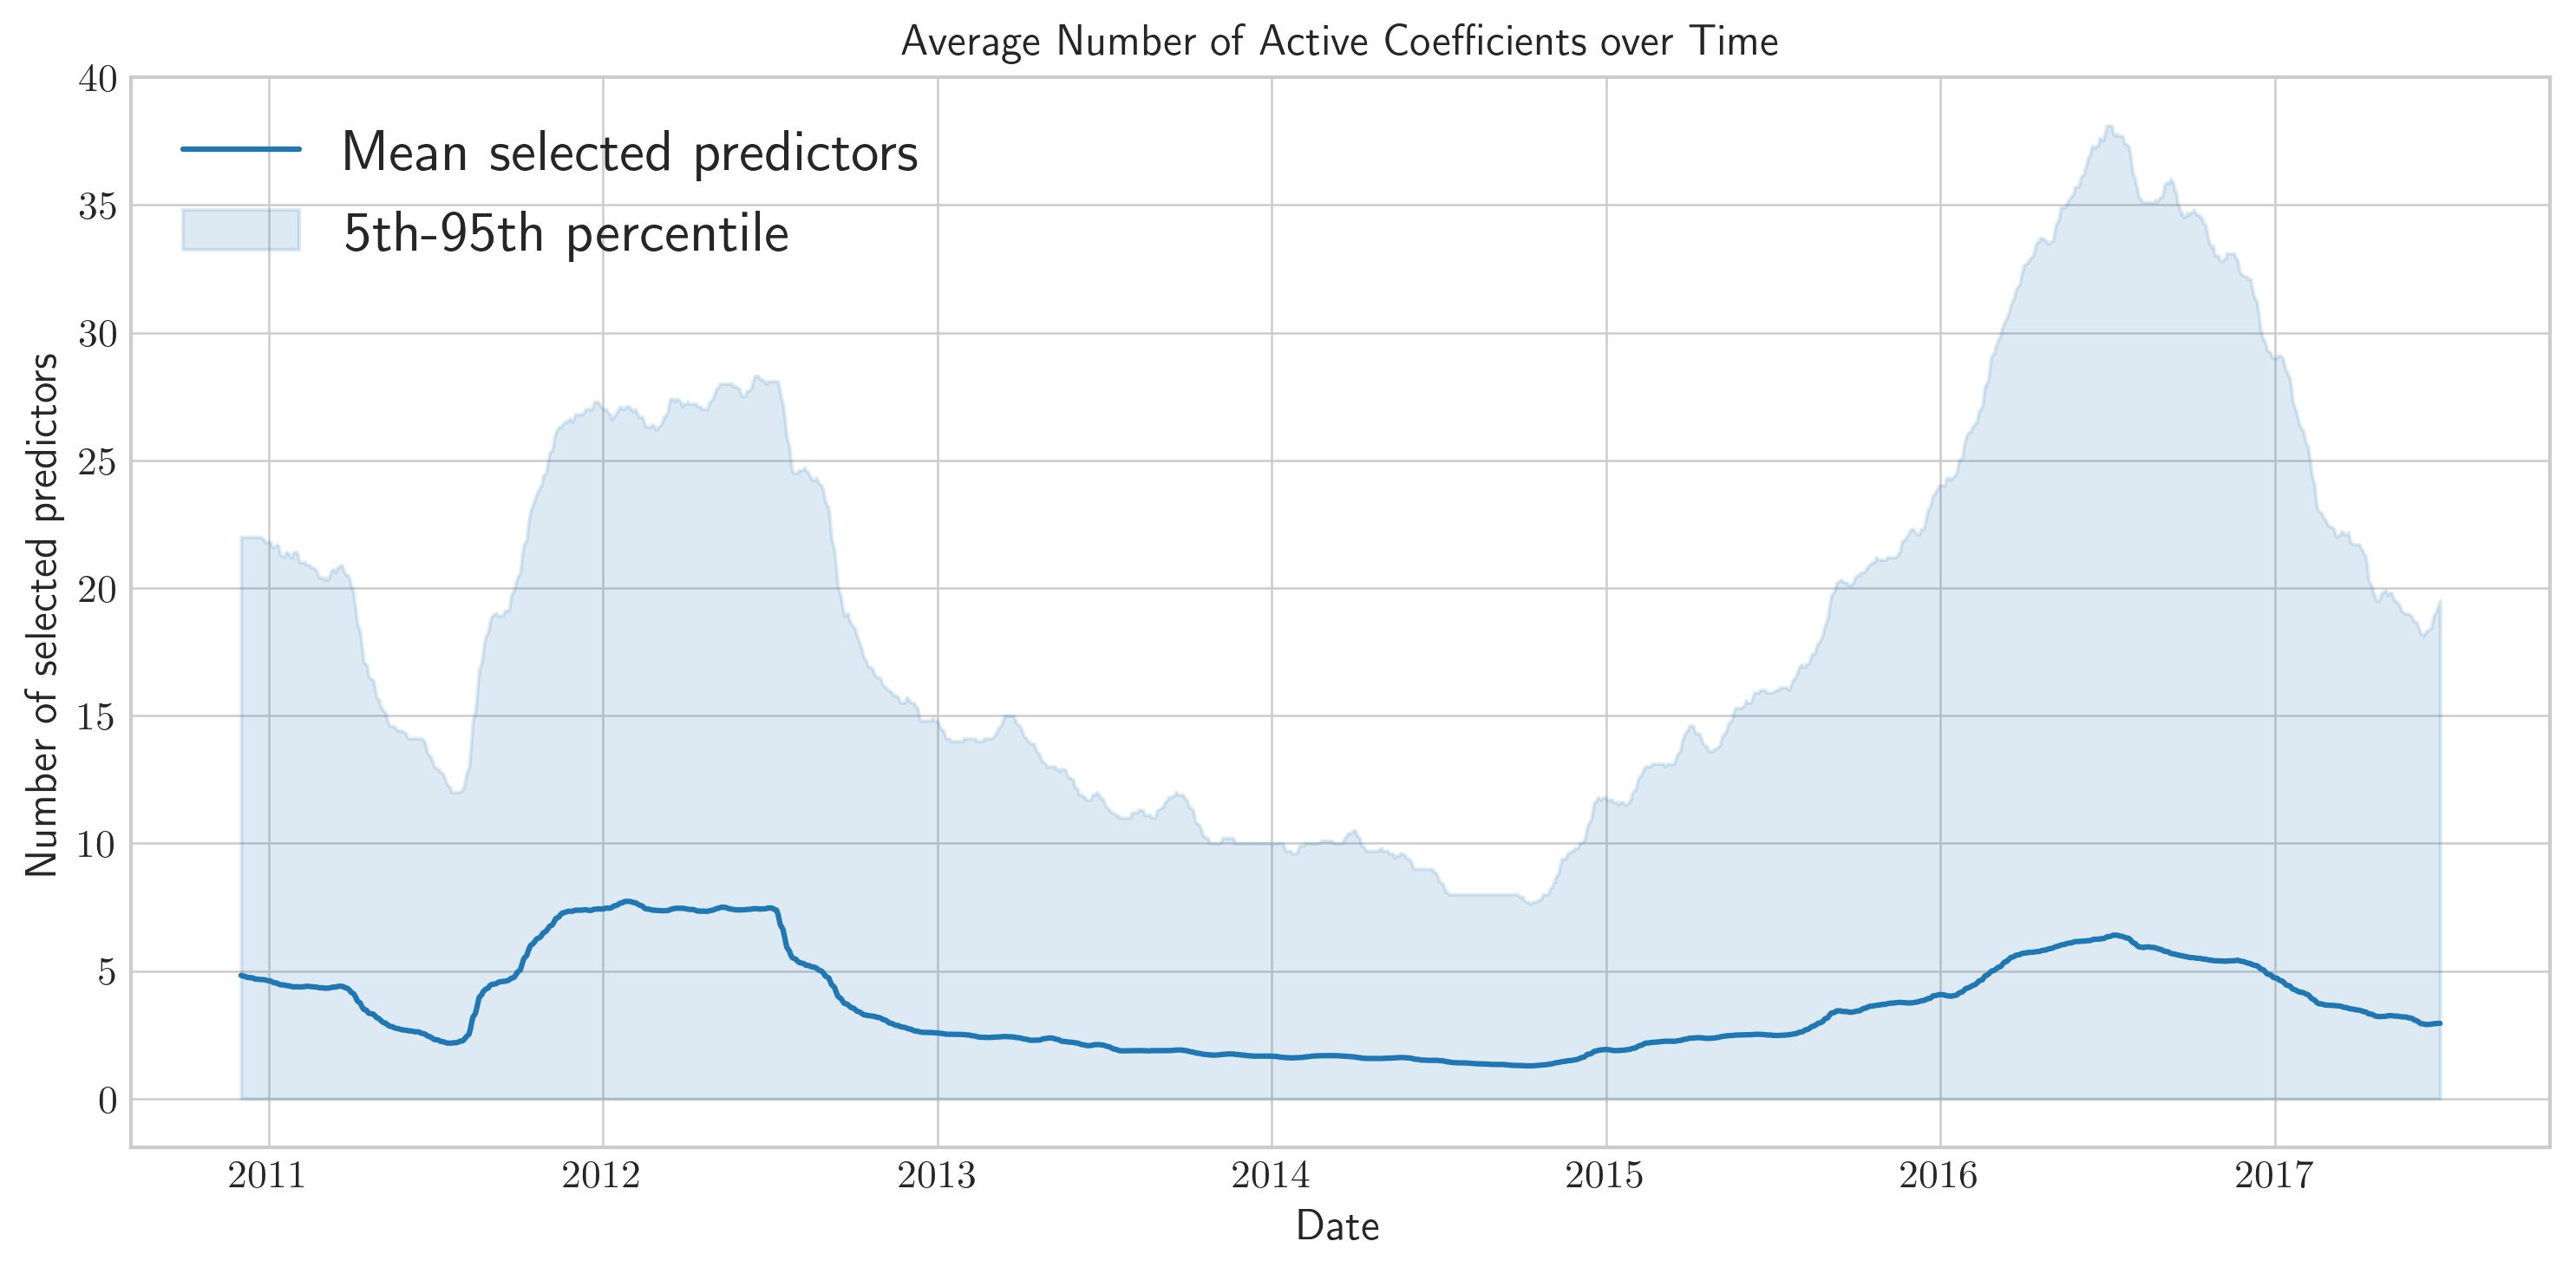
\includegraphics[width=0.7\textwidth]{active_coefficients_over_time.png}
    \caption{Time Variation in LASSO Selection Intensity}
    \label{fig:selection_rate_time}
    \begin{minipage}{\textwidth}
    \footnotesize
    % \textit{Note:} The figure plots the cross-sectional mean number of predictors selected by the LASSO on each trading day. The shaded region denotes the 10th--90th percentile range across stocks. All series are smoothed using a 21-day moving average. Vertical lines mark selected macro-financial events.
    \end{minipage}
\end{figure}

\paragraph{Cross-Sectional Variation.}

Proposition~\ref{prop:LASSO_estimate} implies that under a common penalty, stocks with more volatile returns should be more likely to generate non-zero LASSO coefficients. Figure~\ref{fig:avg_select} plots, for each stock, the mean LASSO selection rate against its idiosyncratic volatility $\hat{\sigma}_i$, measured as the standard deviation of Stage-2 residuals.
Stocks with a statistically significant $\hat{\kappa}$ estimate (at the 5\% level) are highlighted in red.
The relationship is strongly positive and convex: stocks with low idiosyncratic volatility are almost never selected, while the most volatile stocks are selected in upwards of 15\% of rolling windows.

\begin{figure}[h]
\centering
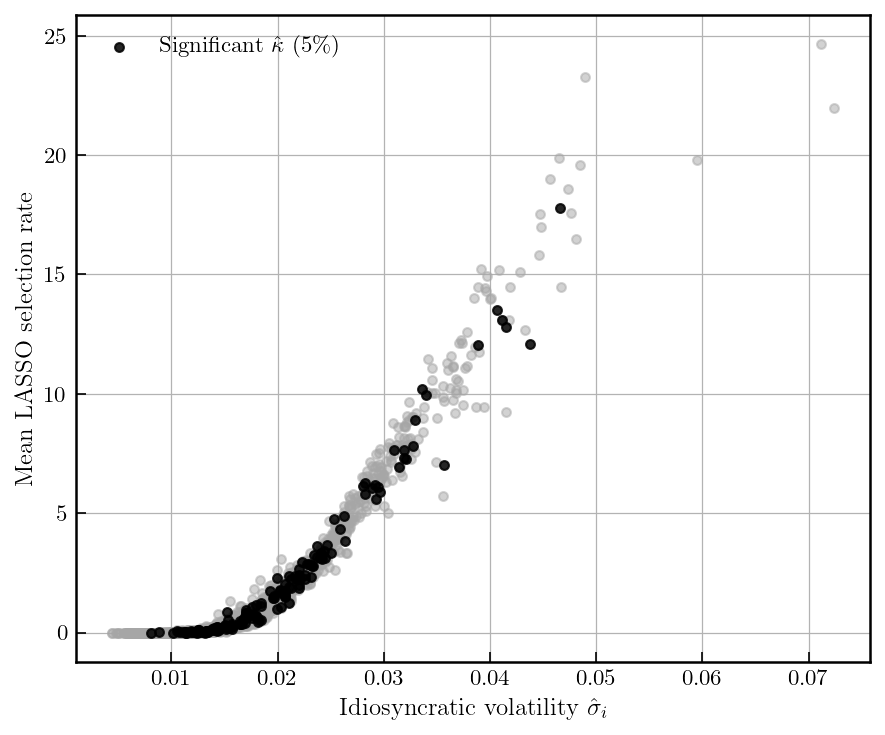
\includegraphics[width=0.7\textwidth]{scatter_idio_vol_selection_r2.png}
\caption{Mean LASSO Selection Rate vs.\ Idiosyncratic Volatility}
\label{fig:avg_select}
\end{figure}

% These patterns suggest that the estimated beliefs are sparse, episodic, and heterogeneous across stocks. The learning rule delivers some in-sample fit, while its out-of-sample performance remains weak, as documented above. This combination is consistent with the model's benchmark in which agents perceive temporary predictability from finite samples even though stable out-of-sample predictability is absent. The results also parallel the evidence in \citet{Chinco2019}, where return predictability appears in short-lived and shifting pockets rather than as a stable forecasting relation.

We next examine \emph{which} features the LASSO selects. 
Again, Proposition~\ref{prop:LASSO_estimate} provides a testable prediction: features with higher volatility should be selected less frequently.
However, since topic-attention innovations are standardized before entering the rolling estimation window, no feature is mechanically more likely to be selected than any other.
Selection should therefore be approximately uniform across features.
To test this, we define the mean selection rate as the fraction of stock-window observations for which the corresponding LASSO coefficient is non-zero.
We compute the rate for each of the 190 predictors. 

Figure~\ref{fig:topic_selection_freq} ranks the 190 candidate features by mean selection rate. Selection is moderately concentrated, with a Gini coefficient of 0.18, but remains dispersed. Every feature is selected at least once, and the most frequently selected feature, \textit{Announce plan}, is selected at $3.1$ times the equal-selection benchmark. The 10 macro-financial series are selected at a rate only marginally higher than the 180 news-topic features ($1.1\times$ on average), suggesting that the modest premium cannot be attributed to a structural advantage of macro series over news topics. The two most frequently selected features, \textit{Announce plan} and \textit{Financial reports}, are both news topics with clear economic interpretations as signals of corporate activity and earnings news.
Overall, no small subset of features dominates the learning rule. Instead, selection is dispersed, with moderate concentration in economically interpretable predictors. Appendix~\ref{app:robustness_sig_kappa} shows that the same pattern holds when the analysis is restricted to the stocks with a statistically significant $\hat{\kappa}$ estimate.

\begin{figure}[h]
    \centering
    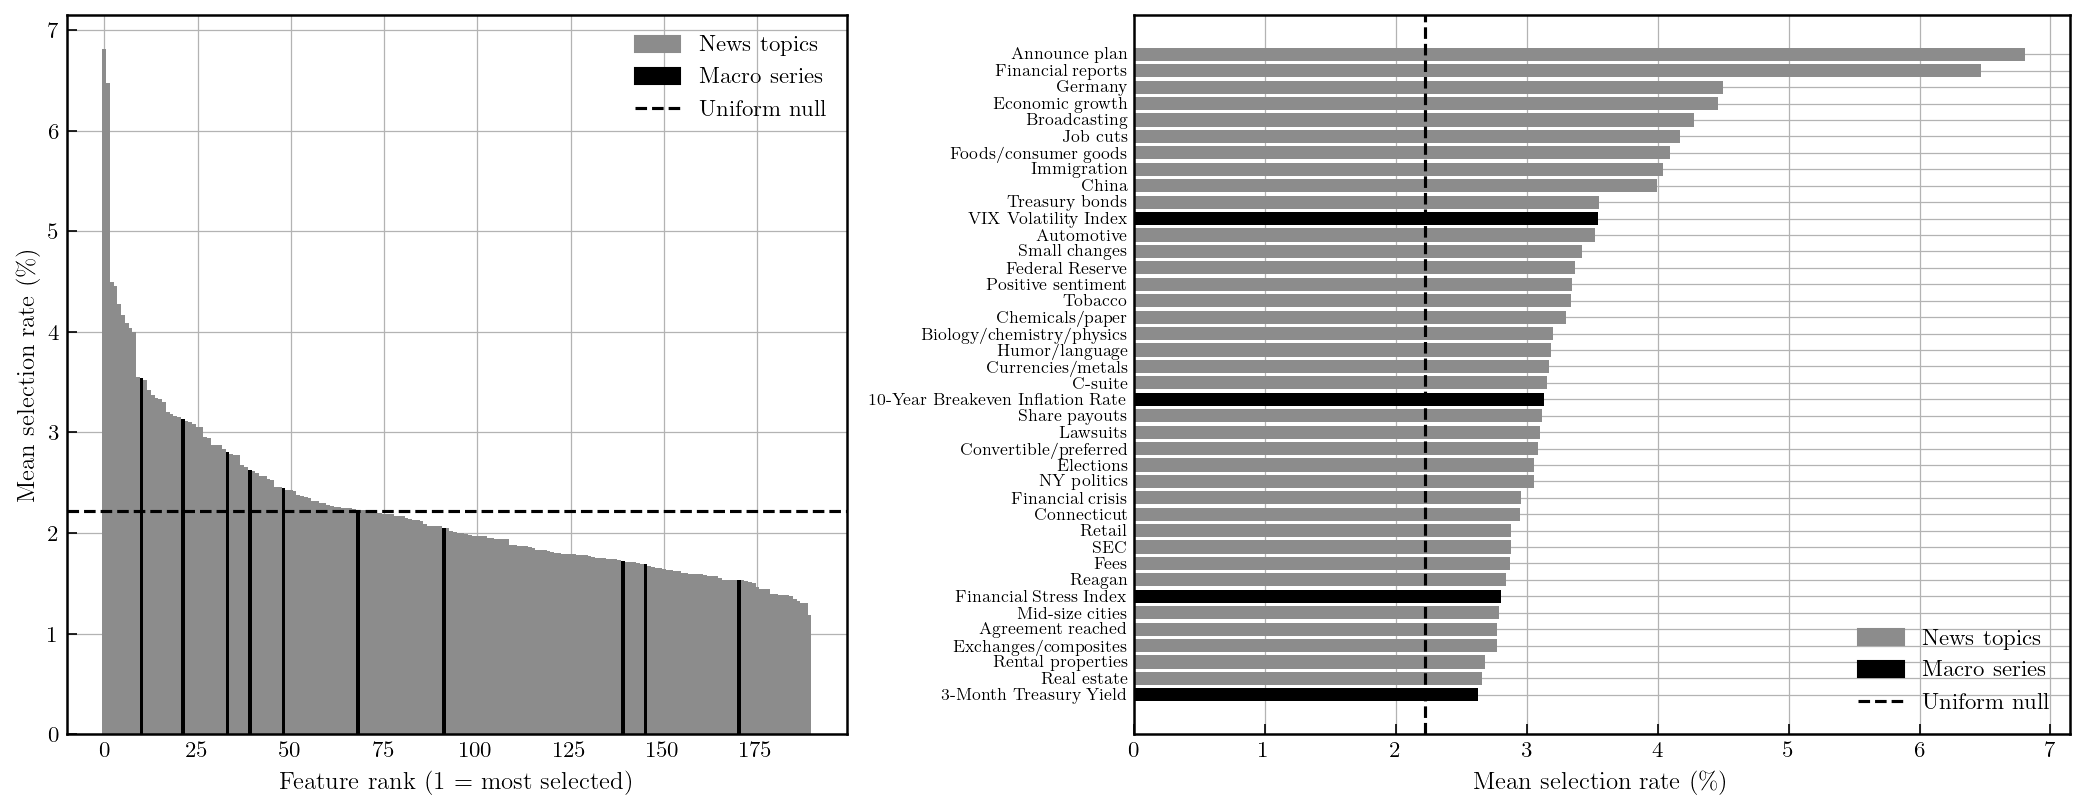
\includegraphics[width=\textwidth]{selection_frequency.png}
    \caption{LASSO Selection Frequency Across Features}
    \label{fig:topic_selection_freq}
    \begin{minipage}{\textwidth}
    \footnotesize
    \textit{Note:} Bars show mean feature selection rates, defined as the share of stock-days with a non-zero LASSO coefficient. Features are ordered by selection frequency; red bars denote macro-financial series and blue bars denote news topics. The dashed line marks the uniform-selection benchmark. The left panel shows all 190 features, while the right panel reports the top 30.
    \end{minipage}
\end{figure}

Figure~\ref{fig:topic_selection_by_stock} plots the distribution of average selected features per rolling window across the 1{,}296 estimation stocks. The distribution is strongly right-skewed, with a substantial mass near zero: approximately 40\% of stocks have an average selection rate below 0.3\%, consistent with the LASSO penalty being especially restrictive for lower-volatility stocks. Together with Figure~\ref{fig:topic_selection_freq}, these results show that sparsity is a structural feature of the data in two dimensions: agents typically select only a sparse subset of features for any individual stock, and the degree of selection varies substantially across the cross-section.


\begin{figure}[h]
    \centering
    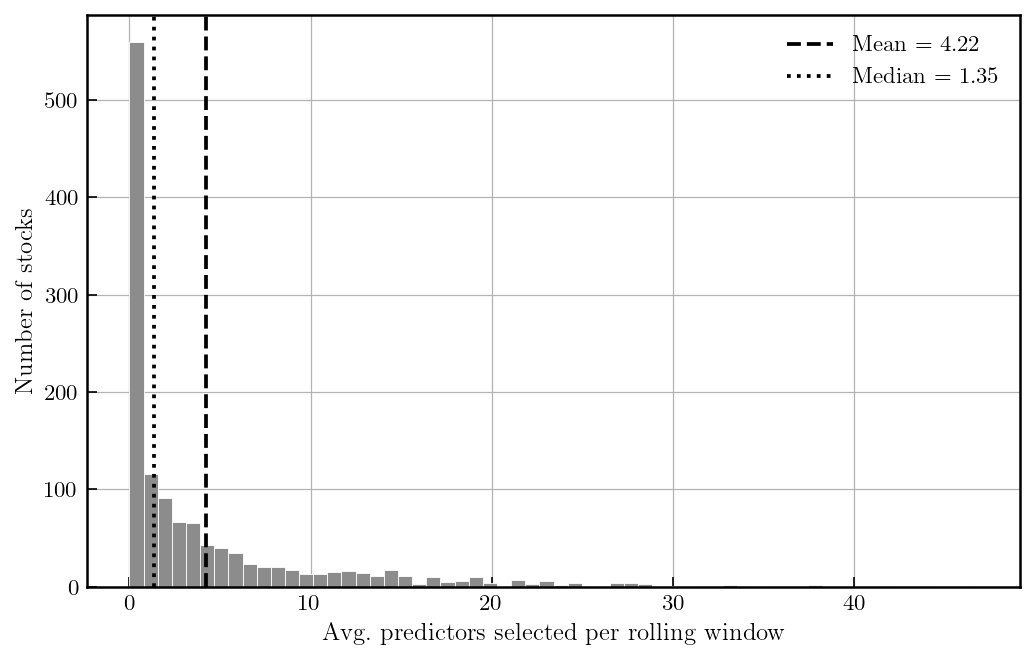
\includegraphics[width=\textwidth]{selection_intensity.png}
    \caption{LASSO Selection Intensity Across Stocks}
    \label{fig:topic_selection_by_stock}
    \begin{minipage}{\textwidth}
    \footnotesize
    \textit{Note:} Histogram of the average number of features selected per rolling window across the 1{,}296 estimation stocks. Dashed line: cross-sectional mean. Dotted line: median.
\end{minipage}
\end{figure}

\paragraph{Persistence.}

Figure~\ref{fig:topic_selection_persistence} shows that topic selection is highly persistent. Pooled across 547{,}907 selection episodes, the run-length distribution is strongly right-skewed: the median episode lasts only 4 windows, yet the 95th percentile reaches 79 windows and some episodes persist for over 600 windows. The survival curve declines from 73\% after one window to 18\% after 20 windows, before flattening into a heavy tail. 
To further quantify persistence, we define a selection indicator $s_{i,j,t} = \mathbf{1}(\hat{\beta}_{i,j,t} \neq 0)$ for each stock--feature pair $(i,j)$ and window $t$. The first-order autocorrelation of $s_{i,j,t}$, averaged across 72{,}882 active stock--feature pairs, is 0.89, decaying slowly to 0.73 at lag 5 and 0.46 at lag 20. While most episodes are short-lived, a minority of topic--stock pairs exhibits highly persistent selection, consistent with the self-reinforcing nature of the CMCE mechanism: a selected belief generates returns that sustain the selection signal until the rolling window rolls past the episode. This is in line with Remark~\ref{rem:persistence} in Section~\ref{sec:lasso}
Appendix~\ref{app:robustness_sig_kappa} confirms that the same pattern holds when restricting to stocks with a statistically significant $\hat{\kappa}$ estimate.

\begin{figure}[h]
    \centering
    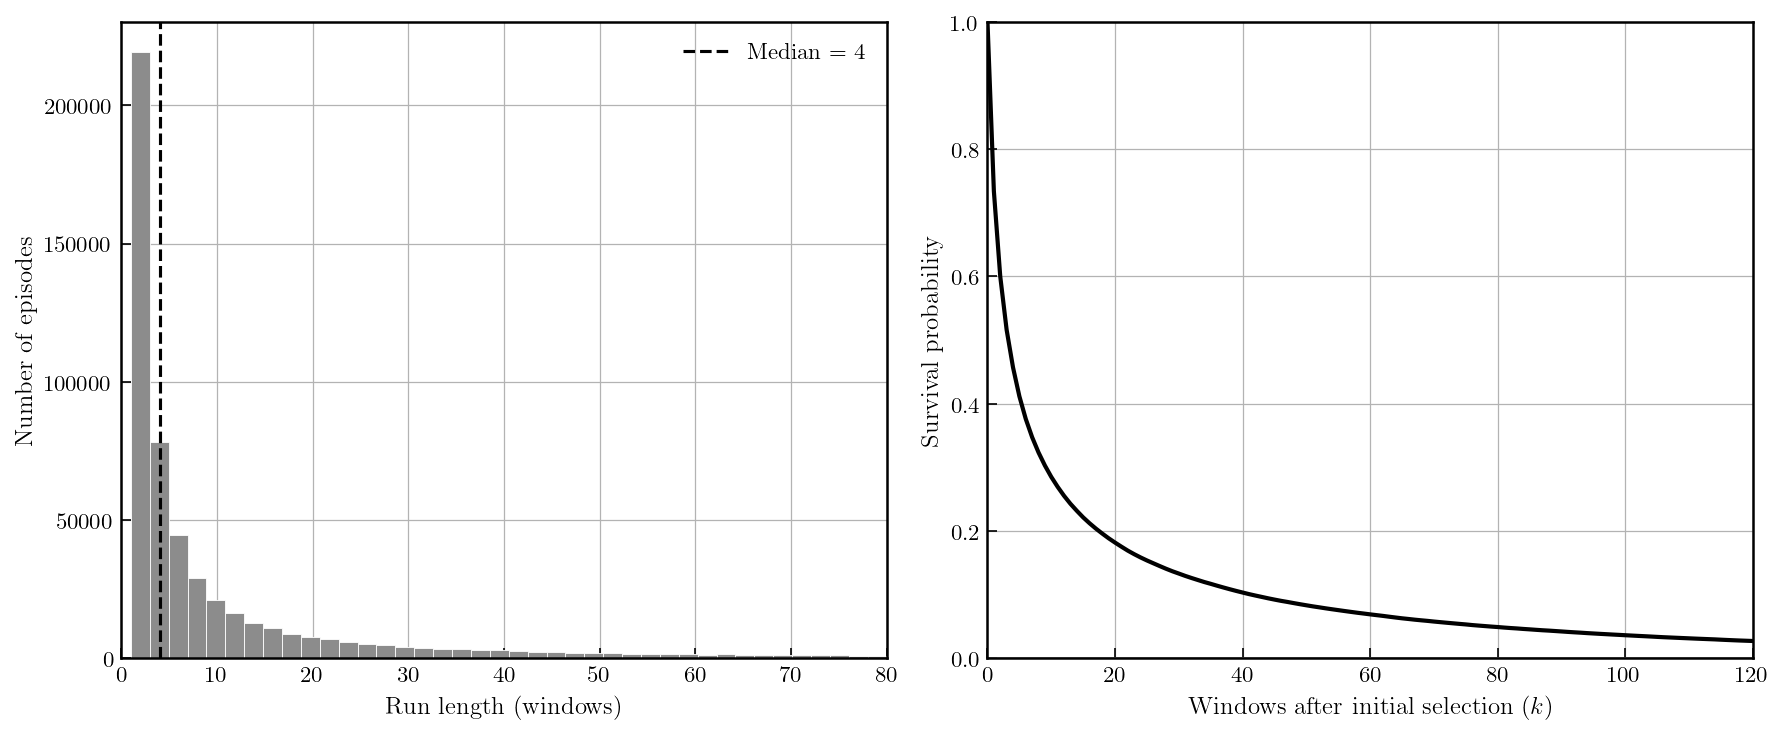
\includegraphics[width=\textwidth]{distribution_survival_autocorrelation.png}
    \caption{Persistence of Topic Selection Episodes}
    \label{fig:topic_selection_persistence}
    \begin{minipage}{\textwidth}
    \footnotesize
    \textit{Note:} \textbf{Left panel}: distribution of run lengths (consecutive windows a feature remains selected), pooled across 547{,}907 episodes and truncated at 80 windows. Dashed line marks the median ($=4$). \textbf{Right panel}: survival curve $P(\text{selected at }t+k \mid \text{selected at }t)$, estimated for each onset event and averaged across all stock--feature pairs. Sample: 1{,}296 stocks, 190 predictors, 1{,}626 trading days.
    \end{minipage}
\end{figure}

\subsection{Volatility, Uncertainty, and Selection}
\label{subsec:empirical_uncertainty_volatility}

\paragraph{Selection and Volatility.}

The model implies that LASSO selection should become more likely when the return process is more volatile. Under a fixed penalty parameter $\lambda$, higher return volatility increases the magnitude of sample return--predictor covariances and therefore raises the probability that estimated coefficients clear the selection threshold. By contrast, higher predictor volatility reduces standardized coefficient magnitudes and should lower selection probabilities. The empirical implication is therefore not simply that ``uncertainty'' raises selection in general, but more specifically that return-side uncertainty increases the likelihood of finite-sample relationships crossing the LASSO threshold.

Figure~\ref{fig:selection_rate_time} provides initial descriptive evidence. Feature selection becomes more frequent during periods of heightened aggregate uncertainty. The average number of selected predictors per stock-day is positively correlated with the VIX, a widely used measure of market uncertainty. The Pearson correlation between the two series is $r=0.358$ ($p<0.001$), indicating that periods of elevated market uncertainty are associated with higher rates of feature selection.

\paragraph{Time-series variation in aggregate selection intensity.}

We next examine what drives time-series variation in aggregate selection intensity. In the baseline CMCE equilibrium with constant idiosyncratic volatility $\sigma_u$, the expected selection rate is time invariant. Systematic co-movement between selection rates and observable volatility measures therefore points to variation outside the baseline model.

To decompose the sources of this variation, we first regress the aggregate selection rate $\bar{s}_t$ on two volatility proxies: the cross-sectional standard deviation of daily returns, $\sigma_{r,t}$, and average absolute topic activity, $\sigma_{x,t}$. The LASSO mechanism implies opposite signs for the two variables. Higher return volatility increases the magnitude of sample return--predictor covariances and raises the probability that coefficients clear the selection threshold. Higher predictor volatility, by contrast, lowers standardized coefficient magnitudes and should reduce selection. Consistent with these predictions, a regression with Newey--West standard errors using 20 lags yields $R^2=0.12$. The coefficient on return volatility is positive and significant, $\hat\beta_{\sigma_r}=0.188$ ($p<0.01$), while the coefficient on topic volatility is negative and significant, $\hat\beta_{\sigma_x}=-0.170$ ($p<0.01$).

To evaluate whether the observed time-series variation can be generated by the finite-sample properties of the model alone, we conduct an oracle simulation. We replace actual returns with i.i.d.\ draws from $\mathcal{N}(0,\hat\sigma_{u,i}^2)$ for 150 stocks and re-estimate the rolling LASSO using each stock's estimated penalty parameter and the same window length, $s=231$. Under constant-variance i.i.d.\ noise, the model predicts a time invariant aggregate selection rate. This is what we find: the standard deviation of the simulated selection rate is 19 times smaller than in the data, and the Spearman correlation between actual and simulated selection rates is close to zero, $\rho=0.02$ ($p=0.31$). Thus, i.i.d.\ noise calibrated to the empirical residual variance cannot account for the observed time-series variation in selection intensity.

% \begin{figure}[H]
%     \centering
%     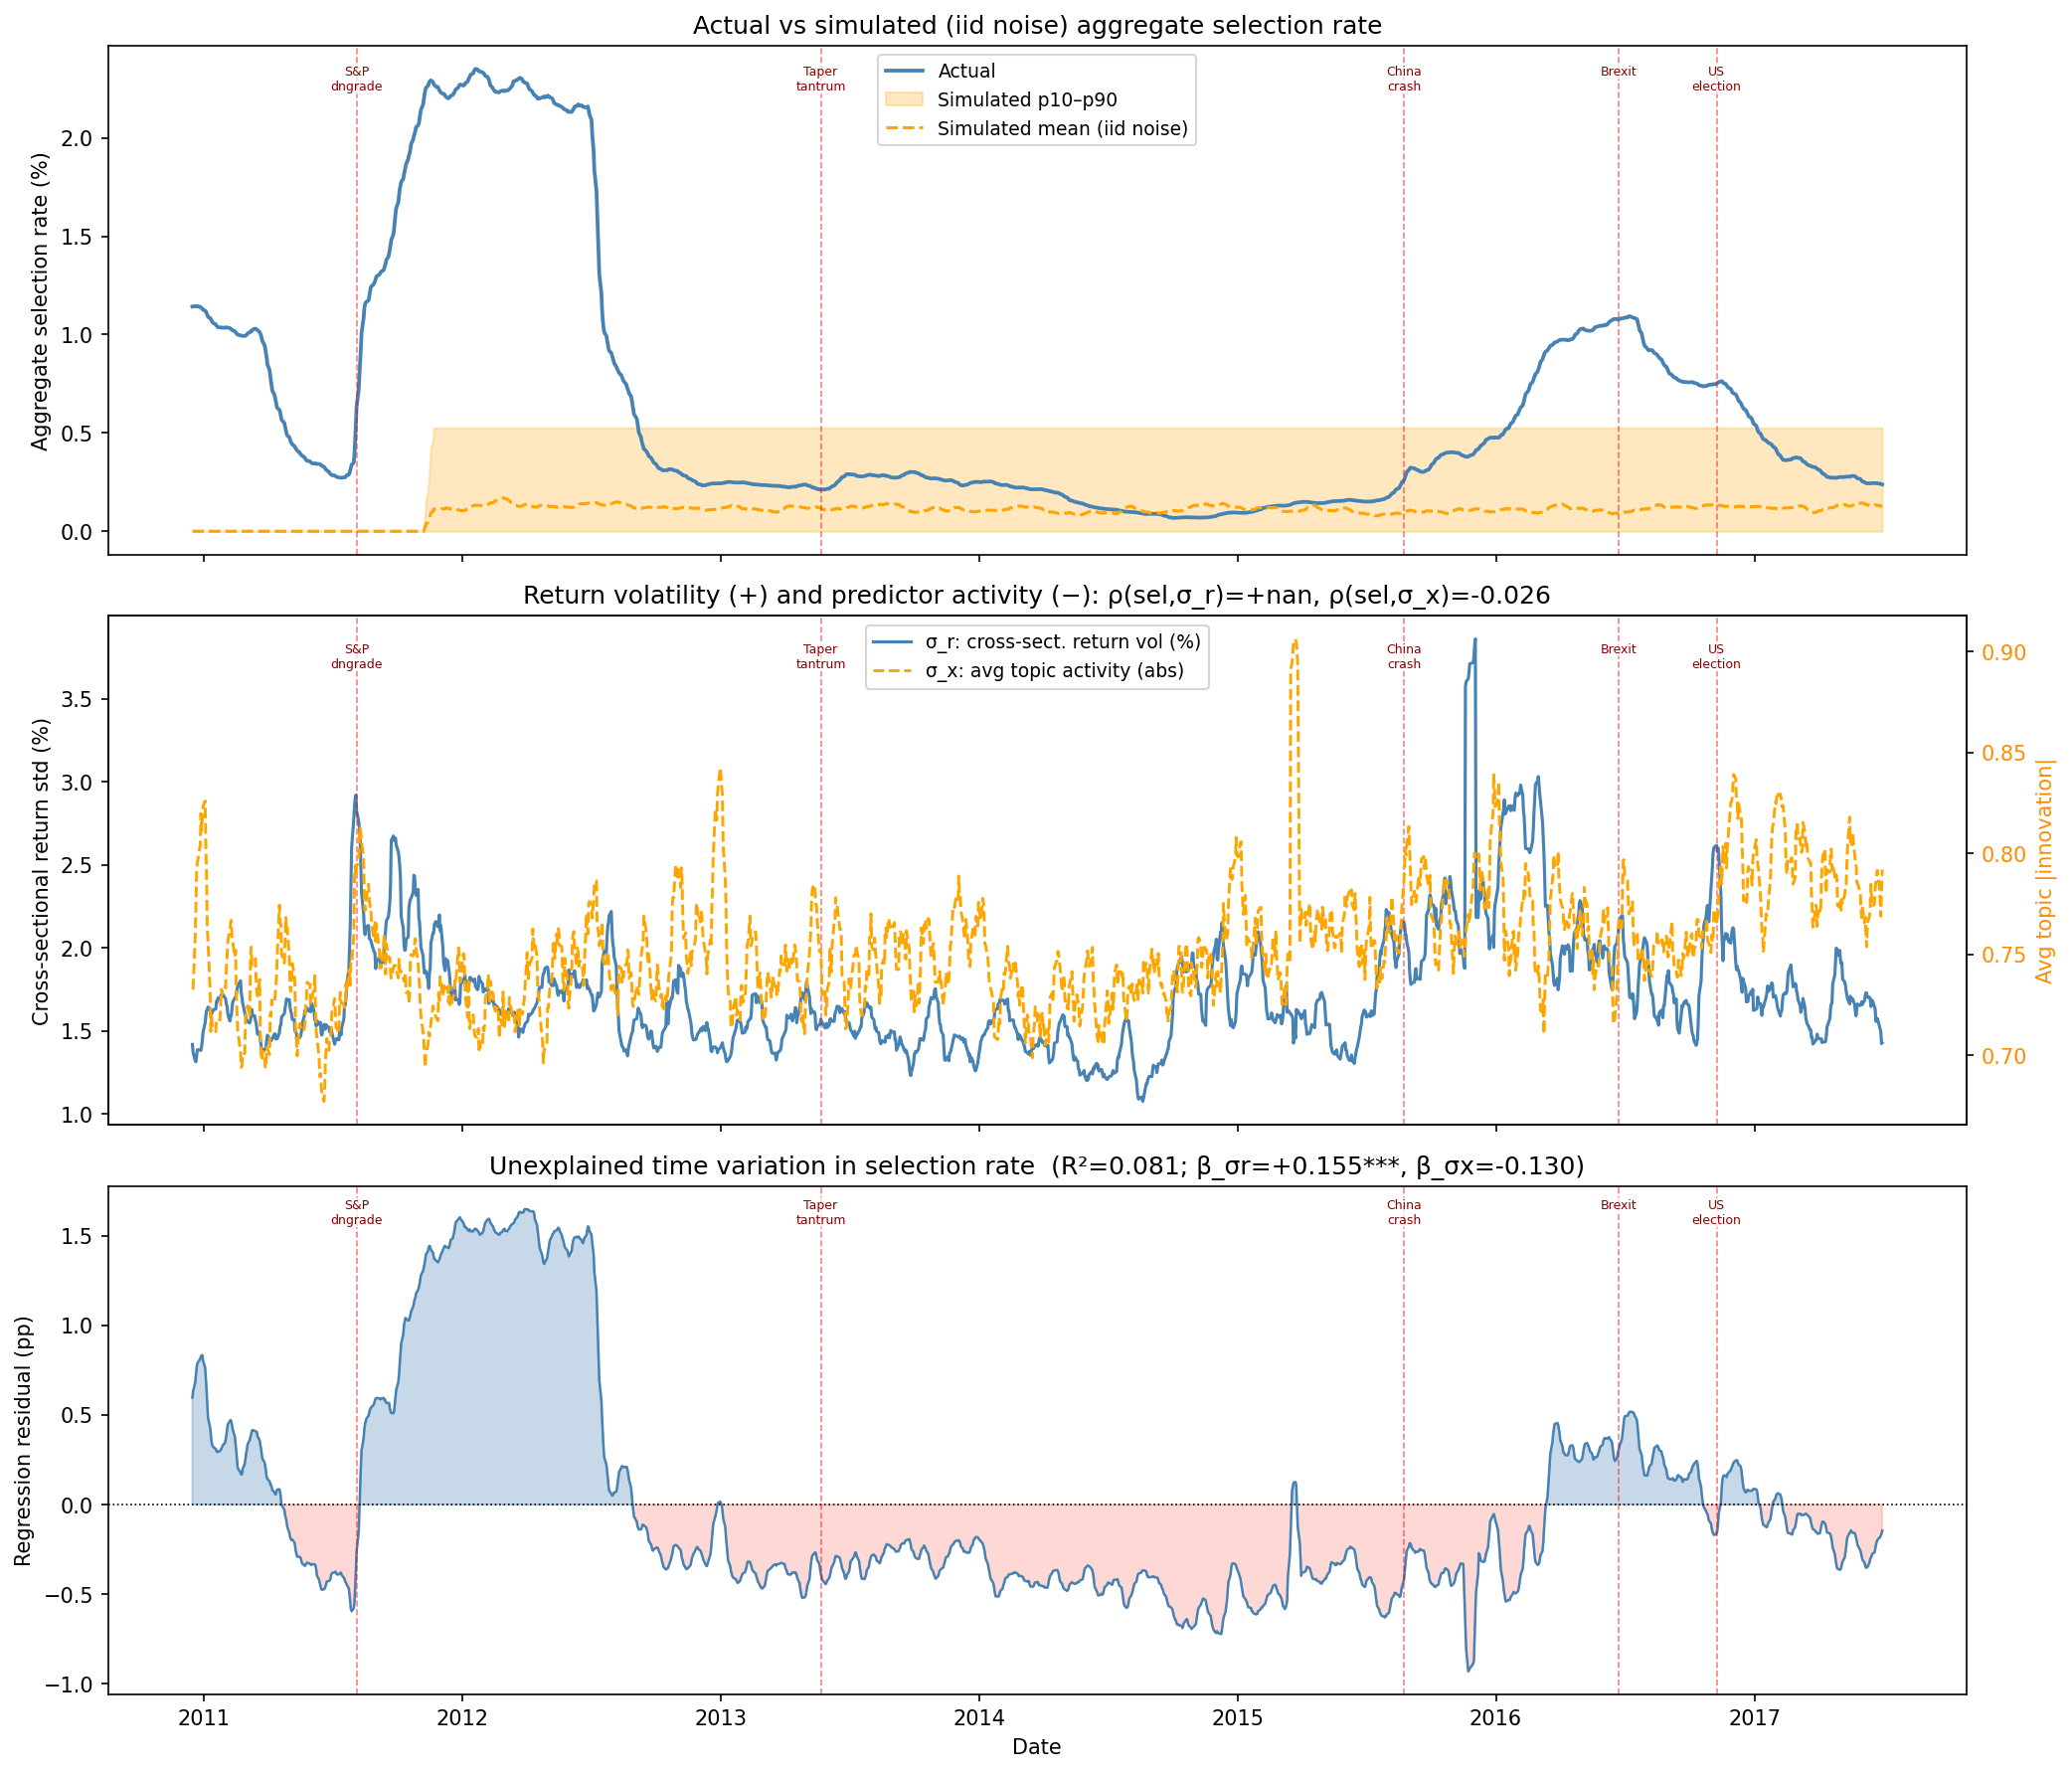
\includegraphics[width=\textwidth]{selection_rate_decomposition.png}
%     \caption{Time-Series Variation in Aggregate Selection Rates}
%     \label{fig:selection_rate_decomposition}
%     \begin{minipage}{\textwidth}
%     \footnotesize
%     \textit{Note:} The top panel compares the actual aggregate selection rate with the i.i.d.\ oracle simulation. The middle panel plots cross-sectional return volatility, $\sigma_{r,t}$, and average absolute topic activity, $\sigma_{x,t}$. The bottom panel reports residuals from the regression
%     $\bar{s}_t = a + b_1\sigma_{r,t} + b_2\sigma_{x,t} + \varepsilon_t$,
%     estimated with Newey--West standard errors using 20 lags. Red dashed lines mark selected macroeconomic events.
%     \end{minipage}
% \end{figure}

\paragraph{Conditional volatility and selection spikes.}

The large gap between actual and simulated selection-rate volatility suggests that the baseline model misses an important feature of the data. We therefore allow the residual return component to exhibit conditional heteroskedasticity. Economically, the residual $u_{i,t}$ captures return variation not spanned by the topic predictors, including earnings surprises, idiosyncratic demand shocks, and liquidity effects. Such residual variation is likely to be state dependent: during periods of macroeconomic stress, both the magnitude and the common component of firm-level shocks tend to increase.
We model this channel using
\[
u_{i,t} = \sigma_{m,t}\eta_t^{(m)} + \tilde\sigma_i\eta_{i,t}^{(i)},
\]
where $\sigma_{m,t}$ follows a GARCH$(1,1)$ process fitted to value-weighted market returns. When conditional market volatility rises, many firms simultaneously experience larger residual shocks. This increases the probability that rolling-window coefficients cross the LASSO threshold, generating aggregate selection spikes even in the absence of stable return predictability.

We quantify this mechanism by simulating 150 stocks with GARCH residuals calibrated to each stock's market beta and idiosyncratic volatility, and then re-running the same rolling LASSO. Relative to the i.i.d.\ oracle, the GARCH oracle matches the data substantially better. The ratio of actual to simulated selection-rate volatility falls from 19.0 under i.i.d.\ noise to 1.32 under GARCH noise. The Spearman correlation between actual and simulated aggregate selection rates rises from $\rho=0.02$ ($p=0.31$) to $\rho=0.38$ ($p<0.0001$). Replacing raw return volatility with the GARCH conditional volatility, $\sigma_{m,t}$, in the regression increases the explanatory power from $R^2=0.12$ to $R^2=0.18$, with $\hat\beta_{\sigma_m}=0.242$ ($p<0.01$) and $\hat\beta_{\sigma_x}=-0.132$ ($p<0.01$).

% \begin{figure}[H]
%     \centering
%     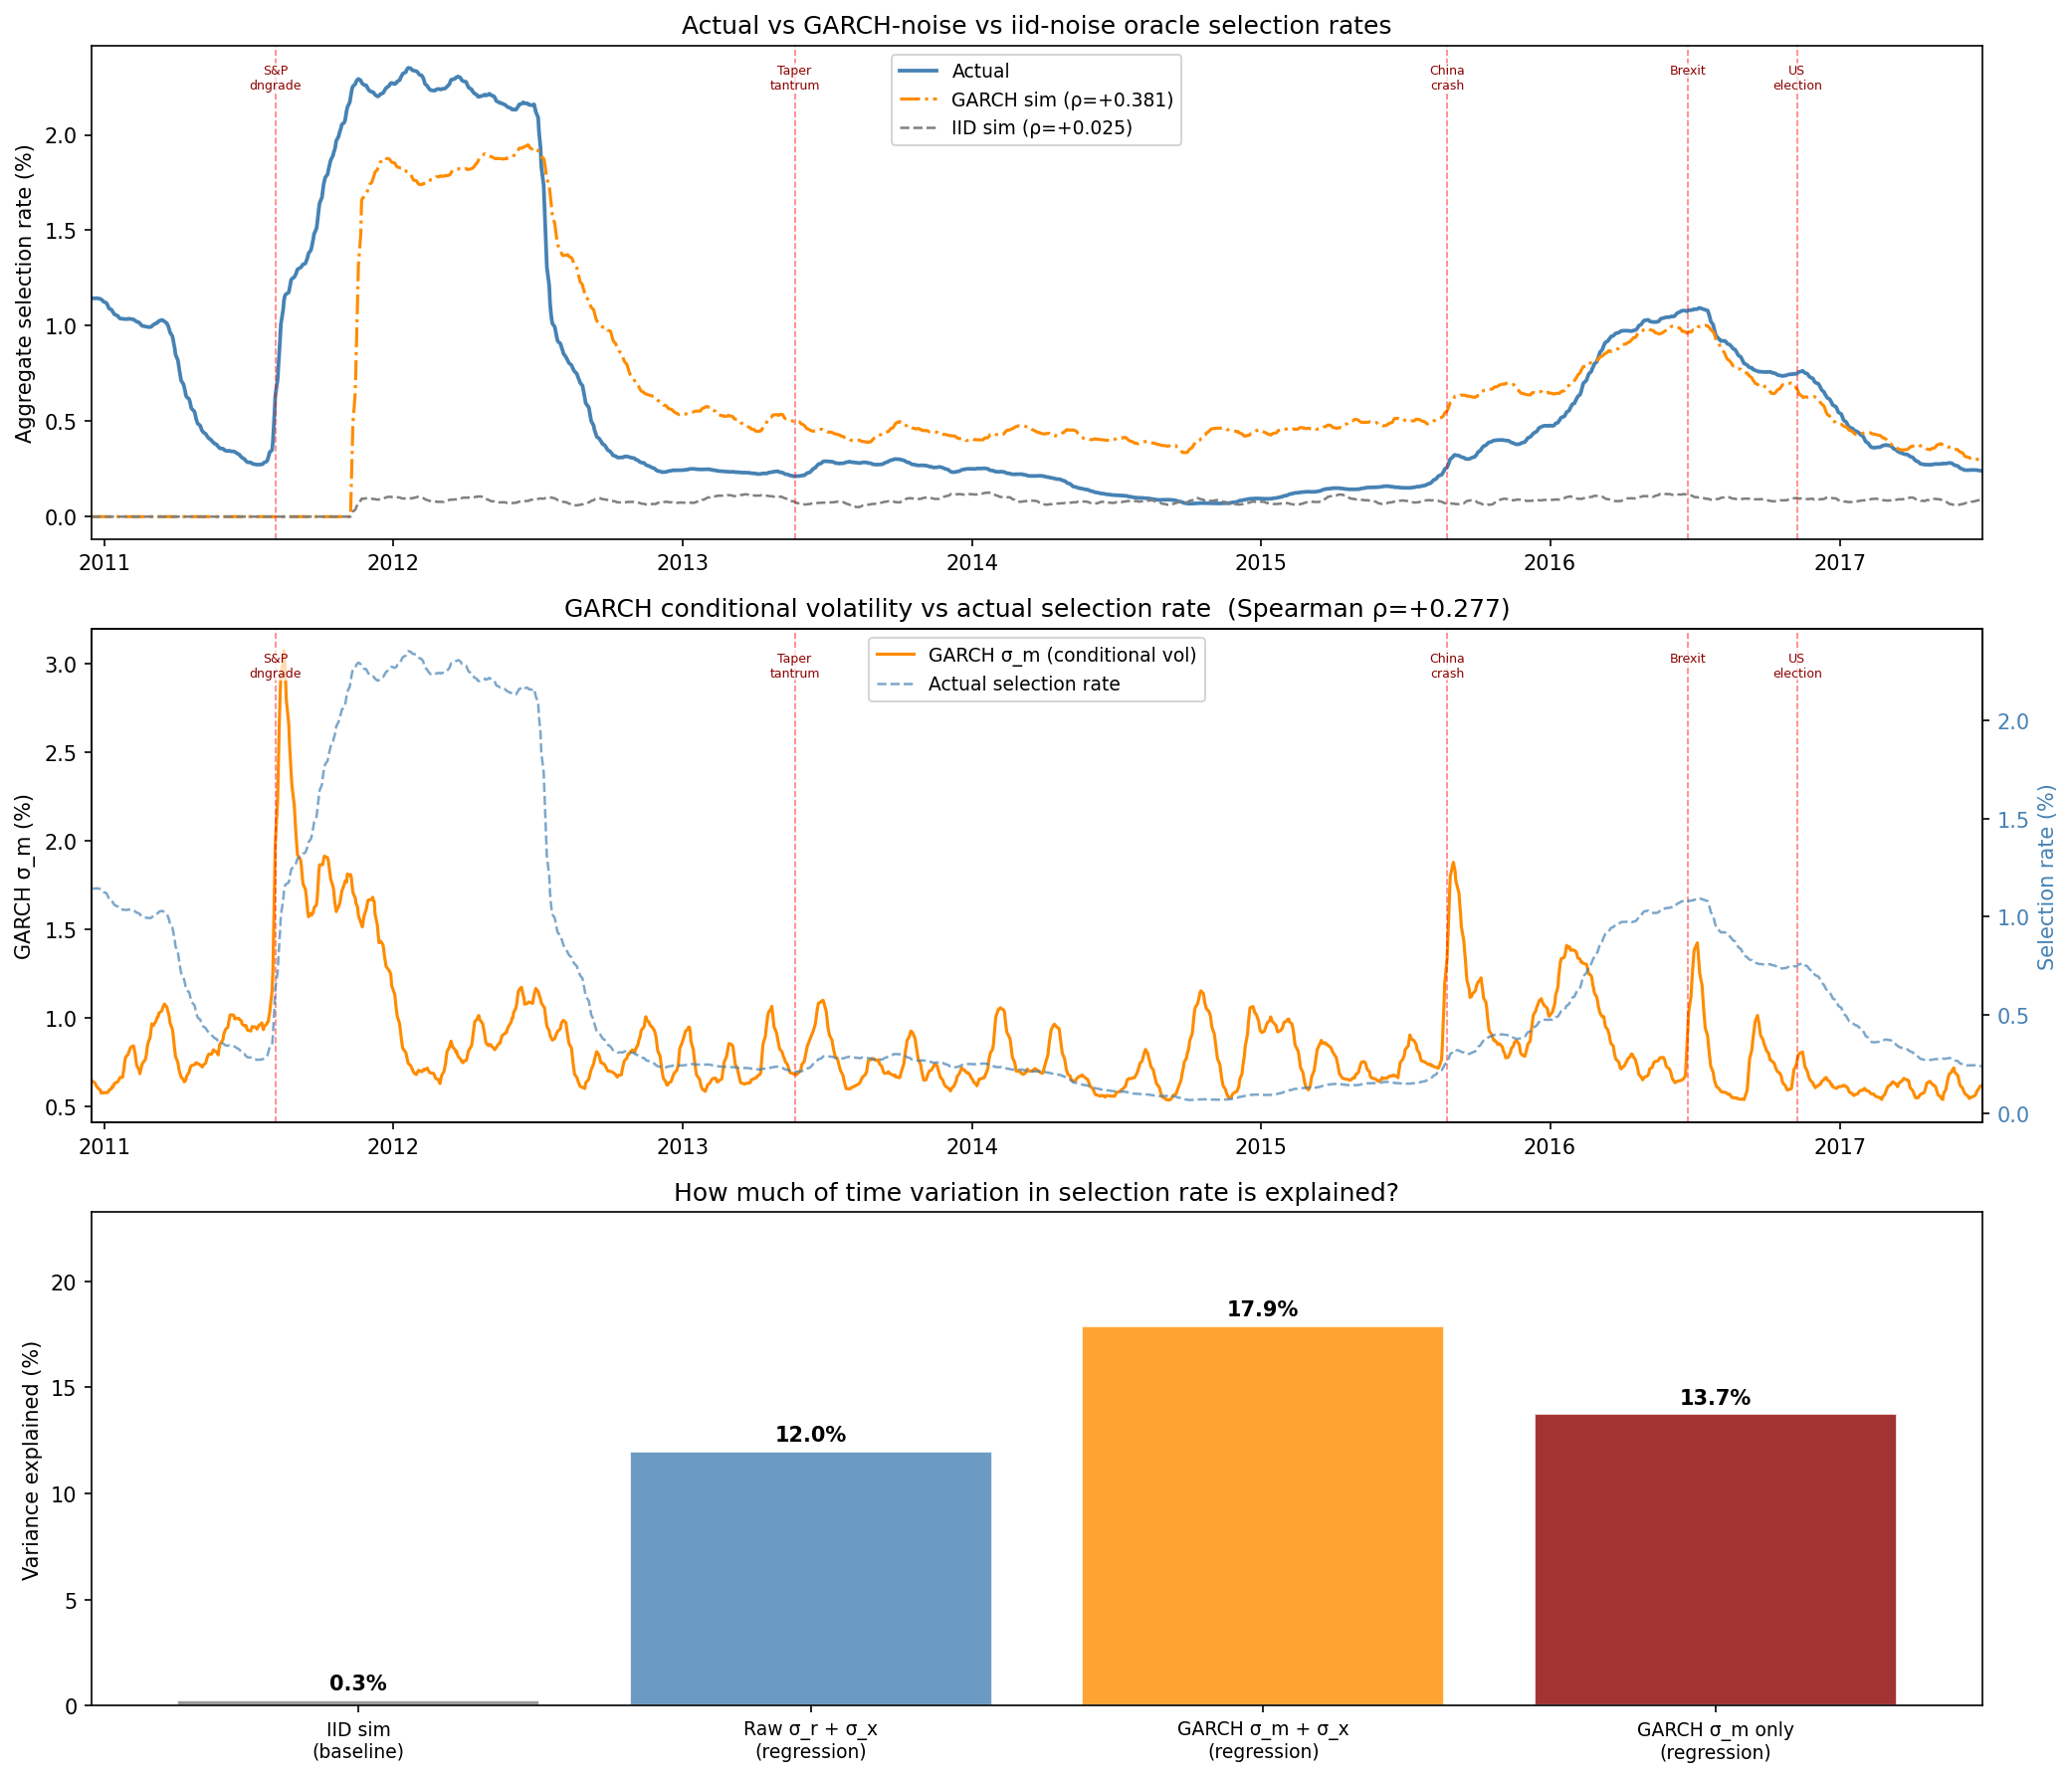
\includegraphics[width=\textwidth]{garch_selection_oracle.png}
%     \caption{Conditional Volatility and Aggregate Selection Rates}
%     \label{fig:garch_oracle}
%     \begin{minipage}{\textwidth}
%     \footnotesize
%     \textit{Note:} The top panel compares the actual aggregate selection rate with the GARCH oracle and the i.i.d.\ oracle. The middle panel plots the GARCH conditional volatility $\hat\sigma_{m,t}$ from a GARCH$(1,1)$ model fitted to daily value-weighted market returns, together with the actual selection rate. The bottom panel reports the fraction of selection-rate variation explained by the i.i.d.\ oracle, the raw-volatility regression, the GARCH-volatility regression, and the GARCH volatility alone. The estimated GARCH persistence parameter is $\hat\alpha+\hat\beta=0.96$.
%     \end{minipage}
% \end{figure}

Taken together, these results indicate that episodic selection spikes are closely linked to time-varying return uncertainty with a common component. The LASSO does not select more topics during high-volatility periods simply because topic activity increases. Rather, conditional return volatility raises the probability that sample relationships cross the selection threshold. The volatility results therefore explain when selection becomes more likely, but not which stock--topic pairs are selected.

\paragraph{Firm-level uncertainty and selection.}

We next ask whether the positive association between uncertainty and selection also appears at the firm level. To do so, we construct a firm-quarter uncertainty index from firms' 10-K filings, measured as the frequency of uncertainty-related terms per 10,000 words, and match it to the quarterly average LASSO selection rate of each firm. Since the distribution of textual uncertainty is highly skewed, all specifications use the log-transformed uncertainty index, standardized within each quarter.

Table~\ref{tab:uncertainty_selection} reports the results. Column~(1) includes firm fixed effects, absorbing all time-invariant firm characteristics, while Column~(2) additionally controls for quarter fixed effects, removing aggregate time-series variation common to all firms. In both specifications a one-standard-deviation increase in log textual uncertainty is associated with a positive and statistically significant increase in the quarterly LASSO selection rate. The coefficient in Column~(1) is 0.18 percentage points ($t=2.07$), indicating that firms with higher reported uncertainty tend to exhibit more active feature selection. Adding quarter fixed effects in Column~(2) yields a coefficient of 0.15 percentage points ($t=1.79$), confirming that the relation holds within firms over time after controlling for aggregate quarterly conditions.
\begin{table}[H]
\centering
\caption{Firm-Level Uncertainty and LASSO Selection}
\label{tab:uncertainty_selection}

\begin{tabular}{lcc}
\toprule
& \multicolumn{2}{c}{Dependent Variable: Selection Rate} \\
\cmidrule(lr){2-3}
& (1) & (2) \\
\midrule
Log Uncertainty Index
    & 0.0018** & 0.0015* \\
    & (0.0009) & (0.0008) \\
\midrule
Firm FE
    & Yes & Yes \\
Quarter FE
    & No  & Yes \\
\midrule
Observations
    & 20,467 & 20,467 \\
Firms
    & 806 & 806 \\
Quarters
    & 26 & 26 \\
$R^2$
    & 0.001 & 0.001 \\
\bottomrule
\end{tabular}

\vspace{0.15cm}
\begin{minipage}{0.95\textwidth}
\footnotesize
\textit{Note:} The dependent variable is the quarterly average LASSO selection rate. The uncertainty index is constructed from 10-K filings, log-transformed, and standardized to have mean zero and unit standard deviation. Both specifications are estimated by panel OLS with firm fixed effects; Column~(2) additionally includes quarter fixed effects. Standard errors are clustered at the firm level. $^{*}p<0.10$, $^{**}p<0.05$, $^{***}p<0.01$.
\end{minipage}
\end{table}
Overall, the firm-level results provide complementary evidence that selection is more common in uncertain information environments. The central mechanism is the volatility channel documented above. Return-side uncertainty raises the probability that finite-sample relationships cross the LASSO threshold.




\section{Are Predictors that are Correlated with the Fundamental Process Selected More Often?}
\label{sec:fundamental_revisions_selection}

The theoretical extension in Section~\ref{sec:correlated_extension} predicts that predictors more strongly correlated with fundamentals should be selected more often. We now provide a direct empirical test of this prediction. The exercise asks whether the stock--predictor pairs for which a predictor is more closely related to innovations in firm fundamentals are also the stock--predictor pairs for which the rolling LASSO selects that predictor more frequently.

\paragraph{Data and identifying assumption.}

We proxy for innovations to firm fundamentals using analyst forecast revisions from I/B/E/S Detail History. The raw data are individual analyst EPS forecasts for U.S. firms between 2010 and 2017, matched to the CRSP PERMNOs in our LASSO estimation sample. We use quarterly EPS forecasts and keep the analyst-level panel before aggregation. A raw observation is indexed by firm $i$, analyst $a$, forecast announcement date $t$, and fiscal-quarter end $\tau$. For each firm--analyst--fiscal-quarter cell, we sort forecasts over time and define the revision
\[
\Delta EPS_{i,a,\tau,t}
= EPS_{i,a,\tau,t}-EPS_{i,a,\tau,t^-},
\]
where $t^-$ denotes the analyst's previous forecast for the same firm and fiscal quarter. We then scale the revision by the previous trading day's absolute CRSP price,
\[
\widetilde{\Delta EPS}_{i,a,\tau,t}
=\frac{\Delta EPS_{i,a,\tau,t}}{|P_{i,t-1}|}.
\]
Finally, we aggregate revisions to the firm-day level,
\[
FundNews_{i,t}
=\frac{1}{N_{i,t}}\sum_{a,\tau}\widetilde{\Delta EPS}_{i,a,\tau,t}.
\]

The identifying assumption is that analyst forecast revisions are timely, noisy signals of innovations to the market's information about firm fundamentals. Analysts revise EPS forecasts when new information changes their assessment of future cash flows. After conditioning on the analyst's own previous forecast for the same firm-quarter, the revision removes the analyst's prior level forecast and isolates the incremental news embedded in the update. Scaling by lagged price makes the revision comparable across firms. This proxy is imperfect: revisions may reflect analyst-specific processing, delayed incorporation of public news, or strategic forecast behavior. The identifying content of the test is therefore not that revisions are structural cash-flow shocks, but that they are monotone in the arrival of fundamental information relevant for firm value.

We date revisions using the I/B/E/S announcement date, mapped to the next CRSP trading day when the announcement falls on a weekend or holiday. This preserves the public-information timing interpretation while avoiding the loss of observations from non-trading-day announcements.

\paragraph{First stage: firm-specific fundamental relevance.}

Let $x_{j,t}$ denote predictor $j$ on trading day $t$. For each revision event date, we construct cumulative predictor innovations over an event window $W$ ending at or before the event date,
\[
X^W_{j,t}=\sum_{s\in W}x_{j,t+s}.
\]
We then estimate a firm-specific time-series regression separately for each firm $i$ and predictor $j$:
\[
FundNews_{i,t}
=a_i+\theta_{i,j}^{W}X^W_{j,t}+\varepsilon_{i,j,t},
\]
using only the revision-event dates of firm $i$. We require at least 50 revision-event observations for a firm to enter the baseline first stage. This threshold balances precision in the generated firm-specific relevance measure against cross-sectional coverage; below we report robustness to alternative thresholds. Fundamental relevance is defined as the absolute first-stage $t$-statistic,
\[
FundRel^W_{i,j}=|t(\hat\theta^W_{i,j})|,
\]
winsorized at the 1st and 99th percentiles within each specification.

For the baseline window $[-5,-1]$, the 50-event cutoff produces 160{,}740 firm--predictor relevance estimates, covering 846 firms and 190 predictors. In the broader event sample, the median firm contributes 165 usable revision-event days, with an interquartile range from 84 to 282.5. The cutoff therefore excludes firms with very sparse analyst-revision histories while retaining most firms with regular analyst coverage.

\paragraph{Second stage: selection rates and fundamental relevance.}

The second-stage outcome is the stock--predictor LASSO selection rate,
\[
SelectionRate_{i,j}
=\frac{1}{T_{i,j}}\sum_t \mathbf{1}\{\hat\beta_{i,j,t}\neq 0\},
\]
computed from the rolling LASSO coefficient tensor used in the main empirical analysis. We merge $SelectionRate_{i,j}$ with $FundRel^W_{i,j}$ and estimate
\[
SelectionRate_{i,j}
=\alpha_i+\delta_j+\beta FundRel^W_{i,j}+u_{i,j},
\]
where $\alpha_i$ are firm fixed effects and $\delta_j$ are predictor fixed effects. The coefficient $\beta$ is identified from within-firm, within-predictor variation in fundamental relevance. Standard errors are clustered two ways by firm and predictor.

Table~\ref{tab:fundamental_relevance_selection} reports the firm-specific results for four event windows. The mean selection rate in the estimation sample is 2.36 percent.

\begin{table}[H]
\centering
\caption{Fundamental Relevance and LASSO Selection}
\label{tab:fundamental_relevance_selection}
\begin{tabular}{lcccc}
\toprule
& \multicolumn{4}{c}{Dependent Variable: $SelectionRate_{i,j}$} \\
\cmidrule(lr){2-5}
Window & $[-5,-1]$ & $[-10,-1]$ & $[-5,0]$ & $[-10,0]$ \\
\midrule
$FundRel^W_{i,j}$
    & 0.000353** & 0.000333*** & 0.000395*** & 0.000343*** \\
    & (0.000144) & (0.000120) & (0.000132) & (0.000120) \\
\midrule
$t$-statistic
    & 2.45 & 2.77 & 2.99 & 2.86 \\
Standardized effect
    & 0.0056 & 0.0060 & 0.0064 & 0.0063 \\
Effect relative to mean selection
    & 1.52\% & 1.43\% & 1.70\% & 1.47\% \\
\midrule
Firm FE
    & Yes & Yes & Yes & Yes \\
Predictor FE
    & Yes & Yes & Yes & Yes \\
Observations
    & 160{,}740 & 160{,}740 & 160{,}740 & 160{,}740 \\
Firms
    & 846 & 846 & 846 & 846 \\
Predictors
    & 190 & 190 & 190 & 190 \\
\bottomrule
\end{tabular}

\vspace{0.15cm}
\begin{minipage}{0.95\textwidth}
\footnotesize
\textit{Note:} The table reports firm-specific event-window estimates requiring at least 50 usable revision-event observations per firm. The first stage regresses signed firm-day EPS forecast revision news, scaled by lagged price, on cumulative predictor innovations over the indicated window, separately for each firm and predictor. $FundRel^W_{i,j}$ is the absolute first-stage $t$-statistic, winsorized at the 1st and 99th percentiles. The second stage regresses the firm--predictor LASSO selection rate on $FundRel^W_{i,j}$ with firm and predictor fixed effects. Standard errors, in parentheses, are clustered two ways by firm and predictor. The standardized effect is $\hat\beta\,sd(FundRel^W)/sd(SelectionRate)$. The effect relative to mean selection is $\hat\beta/\overline{SelectionRate}$. $^{*}p<0.10$, $^{**}p<0.05$, $^{***}p<0.01$.
\end{minipage}
\end{table}

\paragraph{Robustness to the first-stage event-count cutoff.}

The baseline threshold of 50 revision-event days is meant to limit noise in the generated firm-specific relevance measure without restricting attention only to the most heavily covered firms. Table~\ref{tab:fundamental_relevance_cutoffs} reports the baseline $[-5,-1]$ specification under alternative minimum-event thresholds. The coefficient remains positive for every cutoff. Precision improves when moving from 20 to 50 or 100 events, but deteriorates once the cutoff becomes very high because the sample becomes much smaller and increasingly concentrated among large, heavily followed firms. We therefore use 50 events as the baseline and treat the other thresholds as robustness checks.

\begin{table}[H]
\centering
\caption{Robustness to Minimum Revision-Event Cutoff}
\label{tab:fundamental_relevance_cutoffs}
\resizebox{\textwidth}{!}{%
\begin{tabular}{lccccccc}
\toprule
Minimum events & 20 & 50 & 100 & 200 & 300 & 400 & 500 \\
\midrule
$FundRel^{[-5,-1]}_{i,j}$
    & 0.000310** & 0.000353** & 0.000394** & 0.000301 & 0.000544** & 0.000383 & 0.000223 \\
    & (0.000137) & (0.000144) & (0.000153) & (0.000186) & (0.000245) & (0.000338) & (0.000323) \\
$t$-statistic
    & 2.27 & 2.45 & 2.57 & 1.62 & 2.22 & 1.14 & 0.69 \\
\midrule
Firms
    & 924 & 846 & 676 & 391 & 208 & 118 & 78 \\
Observations
    & 175{,}560 & 160{,}740 & 128{,}440 & 74{,}290 & 39{,}520 & 22{,}420 & 14{,}820 \\
\bottomrule
\end{tabular}
}

\vspace{0.15cm}
\begin{minipage}{0.95\textwidth}
\footnotesize
\textit{Note:} The table repeats the baseline $[-5,-1]$ firm-specific specification while varying the minimum number of usable revision-event observations required for a firm to enter the first stage. Standard errors, in parentheses, are clustered two ways by firm and predictor. $^{*}p<0.10$, $^{**}p<0.05$, $^{***}p<0.01$.
\end{minipage}
\end{table}

\paragraph{Robustness to using coefficient magnitudes.}

Our baseline measure uses the absolute first-stage $t$-statistic because it captures the reliability of the firm-specific relation between predictor $j$ and fundamental news for firm $i$. The raw coefficient magnitude $|\hat\theta^W_{i,j}|$ is more directly interpretable as an exposure, but it also depends on the scale and volatility of firm-level EPS revisions. Thus, firms with noisier or more volatile forecast revisions may mechanically have larger coefficient magnitudes even when the predictor is not more reliably related to fundamentals. To check that the baseline result is not an artifact of using $|t|$, we re-estimate the second stage replacing $FundRel^W_{i,j}$ with the winsorized absolute coefficient $|\hat\theta^W_{i,j}|$ from the same firm-specific first-stage regressions.

\begin{table}[H]
\centering
\caption{Robustness: Using Absolute First-Stage Coefficients}
\label{tab:fundamental_relevance_selection_theta}
\begin{tabular}{lcccc}
\toprule
& \multicolumn{4}{c}{Dependent Variable: $SelectionRate_{i,j}$} \\
\cmidrule(lr){2-5}
Window & $[-5,-1]$ & $[-10,-1]$ & $[-5,0]$ & $[-10,0]$ \\
\midrule
$|\hat\theta^W_{i,j}|$
    & 0.4136* & -0.1069 & 0.0909 & 0.1298 \\
    & (0.2121) & (0.2567) & (0.1809) & (0.2333) \\
\midrule
$t$-statistic
    & 1.95 & -0.42 & 0.50 & 0.56 \\
Standardized effect
    & 0.0210 & -0.0039 & 0.0041 & 0.0046 \\
\midrule
Firm FE
    & Yes & Yes & Yes & Yes \\
Predictor FE
    & Yes & Yes & Yes & Yes \\
Observations
    & 160{,}740 & 160{,}740 & 160{,}740 & 160{,}740 \\
Firms
    & 846 & 846 & 846 & 846 \\
Predictors
    & 190 & 190 & 190 & 190 \\
\bottomrule
\end{tabular}

\vspace{0.15cm}
\begin{minipage}{0.95\textwidth}
\footnotesize
\textit{Note:} The table repeats the second-stage specification from Table~\ref{tab:fundamental_relevance_selection}, replacing $FundRel^W_{i,j}=|t(\hat\theta^W_{i,j})|$ with the winsorized absolute first-stage coefficient $|\hat\theta^W_{i,j}|$. Standard errors, in parentheses, are clustered two ways by firm and predictor. The standardized effect is $\hat\beta\,sd(|\hat\theta^W|)/sd(SelectionRate)$. $^{*}p<0.10$, $^{**}p<0.05$, $^{***}p<0.01$.
\end{minipage}
\end{table}

\paragraph{Discussion.}

The estimates are positive across all four windows. This is consistent with the mechanism in Section~\ref{sec:correlated_extension}: predictors that are more closely related to innovations in firm fundamentals are selected more frequently by the rolling LASSO. The baseline pre-event window $[-5,-1]$ yields a coefficient of 0.00035 with a two-way clustered $t$-statistic of 2.45. Extending the pre-event window to $[-10,-1]$ gives a similar estimate, 0.00033, with a $t$-statistic of 2.77. Including the event day strengthens the coefficient for the five-day window: the estimate rises to 0.00040 for $[-5,0]$ and the $t$-statistic increases to 2.99. The corresponding ten-day window $[-10,0]$ remains positive and statistically significant.

The economic magnitudes are small in levels, which is expected because unconditional LASSO selection rates are low. A one-unit increase in fundamental relevance raises the selection rate by roughly 1.4--1.7 percent of the mean selection rate, depending on the window. Standardized effects are also modest, around 0.6 percent of a standard deviation in selection rates. The results should therefore not be read as implying that analyst-revision fundamentals are the dominant determinant of selection. Rather, they show that the identity of selected predictors is not purely arbitrary: within firm and within predictor, the pairs with stronger links to measured fundamental-news revisions are selected more often.

The timing pattern is informative. The effect is present using only pre-event predictor innovations, which mitigates the concern that the relation is entirely contemporaneous. At the same time, the stronger $[-5,0]$ estimate suggests that part of the relevant information arrives on the revision day itself, consistent with analysts updating forecasts in response to same-day public news. Table~\ref{tab:fundamental_relevance_cutoffs} shows that the baseline result is not driven by the 50-event threshold: the coefficient remains positive for cutoffs from 20 to 500 events, although precision falls at very high cutoffs as the sample shrinks. The coefficient-based robustness check in Table~\ref{tab:fundamental_relevance_selection_theta} is weaker: the baseline $[-5,-1]$ estimate remains positive and marginally significant, but the longer-window coefficient specifications are not stable. This pattern is consistent with the interpretation that raw coefficient magnitudes are contaminated by cross-firm differences in the volatility of EPS revisions, whereas the $t$-statistic better captures the reliability of the predictor--fundamental-news relation. Overall, the evidence supports the paper's interpretation that finite-sample LASSO selection is amplified when candidate predictors are genuinely correlated with the firm's fundamental information process, while also suggesting that the signal is measured with substantial noise.

\section{Conclusion}\label{sec:conclusion}

This paper develops an asset-pricing model in which investors search for return predictability in a high-dimensional information environment using a LASSO-based learning rule.
Agents estimate a penalized linear forecasting model, form expectations based on the selected predictors, and these beliefs feed back into prices through a nonlinear asset-pricing equation.
Because perceived and actual laws of motion differ, learning does not converge to rational expectations; instead, the economy settles into a cross-moment consistent equilibrium (CMCE).
The central implication is that the act of searching for predictability can itself generate sparse and short-lived windows of return predictability.
In finite samples, agents occasionally select predictors by chance.
When this occurs, trading on the perceived signal feeds back into prices, making the predictability temporarily self-fulfilling.
As new data arrive and older observations drop out of the agents’ effective memory, coefficient estimates revert back to zero, and the induced predictability disappears.
The theory yields tractable conditions linking the frequency of selection events to fundamentals and features of the information environment.
Empirically, we implement the model on daily returns for 1{,}620 NYSE-listed stocks from 2010--2017 using 180 Wall Street Journal news-attention innovations as predictors.
Consistent with the model, predictability is episodic and sparse, and selection occurs more frequently for higher-volatility stocks.


We plan to extend our analysis along several dimensions.
The current model features a representative agent; a natural next step is to introduce heterogeneity in learning behavior.
On the empirical side, the model cannot explain heterogeneity in the probability that different features are selected, beyond what is implied by their statistical properties. 
The data, however, exhibit systematic cross-feature variation in selection frequencies. 
We therefore test whether this variation reflects an additional, non-statistical component of behavior. 
Specifically, we hypothesize that, after estimating the statistical model, agents are more likely to act on its signals when the resulting predictions are consistent with their pre-existing narratives about how the stock market works and about plausible causal links between specific features and asset prices.



% =====================================================


\newpage
\bibliography{references}
\newpage
\appendix
\section{Derivation of Recursive Learning Models}\label{sec:appendix_learning}
\subsection{Recursive Least Squares}\label{app:RLS}

The first updating mechanism we consider is Recursive Least Squares (RLS), which is a recursive implementation of the standard Ordinary Least Squares (OLS).
In OLS, the agent estimates the coefficients of a linear regression model by minimizing the sum of squared residuals.
Assuming agents use OLS to estimate the parameters in the PLM (\ref{eq:plm_univariate}), the OLS estimator $\beta_t$ can be derived from the minimization\footnote{
We use the following timing:
at time $t$ the agent forecasts $r^e_{t+1} = x_t \beta_{t}$ which then implies a realization for $r_t$. 
Therefore, to avoid simultaneity issues, we assume that when computing the current estimate, the last available log-return observation is $r_{t-1}$.
} problem as
\begin{equation}
     \beta_t = \left(\sum^{t-1}_{i=1}  x_{i-1}^2 \right)^{-1} \sum^{t-1}_{i=1}  x_{i-1} r_i.
\end{equation}

Estimating OLS on the whole available data set is sometimes referred to as off-line estimation. 
Another approach is to estimate the model on-line, that is, as soon as a new data point arrives. 
It turns out that the estimator formula allows for a recursive formulation.
Define 
\begin{equation}
M_{t-1} = \frac{1}{t-1}  \left(\sum^{t-1}_{i=1}  x_{i-1}^2 \right), \quad \beta_t = \frac{1}{t-1} M^{-1}_{t-1} \sum^{t-1}_{i=1}  x_{i-1} r_i.
\end{equation}

First we establish a recursion for $M_t$. Start from 
\begin{equation}
\frac{t-1}{t} M_{t-1} = \frac{1}{t}  \left(\sum^{t-1}_{i=1}  x_{i-1}^2 \right) \implies \frac{t-1}{t} M_{t-1} + \frac{1}{t} x_{t-1}^2 = M_t,
\end{equation}
that is
\begin{equation}
    M_t = M_{t-1} + \frac{1}{t} \left(x_{t-1}^2 - M_{t-1} \right).
\end{equation}

For $\beta_t$ we have
\begin{equation}\label{eq:b_t_evolution}
    \begin{aligned}
        \beta_t & = \beta_{t-1} + \left[(t-1) M_{t-1} \right]^{-1} \left\{ x_{t-2} r_{t-1} + \left[(t-2) M_{t-2} \right] \beta_{t-1} \right\} - \beta_{t-1} \\
        & = \beta_{t-1} + \left[(t-1) M_{t-1} \right]^{-1} \left\{ x_{t-2} r_{t-1} - x_{t-2}^2 \beta_{t-1} \right\}.
    \end{aligned}
\end{equation}

\subsection{Constant Gain Learning}\label{app:WLS}
In Weighted Least Squares (WLS), the agent estimates the coefficients of a linear regression model by minimizing a weighted sum of squared residuals.
The weights are typically chosen to reflect the relative importance or reliability of different observations. Assuming the linear model (\ref{eq:plm_univariate}),
the WLS estimator can be derived from the minimization problem
\begin{equation}
    \min_{\beta} \sum^{t-1}_{i=1} {w_{t-1,i}} (r_i - \beta x_{i-1}) ^2,
\end{equation}
with solution
\begin{equation}
    {\beta} = \left(\sum^{t-1}_{i=1} {w_{t-1,i}} x_{i-1}^2 \right)^{-1} \sum^{t-1}_{i=1} {w_{t-1,i}} x_{i-1} r_i.
\end{equation}

In particular, we are interested in the case where the weights decline geometrically over time\footnote{
    In empirical applications, instead of using geometrically declining weights, it is common to use a rolling window approach, where only the most recent observations within a fixed-size window are used for estimation. 
    However, the latter is analytically intractable.
    It is possible to determine a relationship between the window size and the geometric decay parameter $\gamma$ such that the two methods give similar weights \emph{overall} on the $\ell$ most recent observations:
    $\ell \approx \log(1 - p) / \log(1 - \gamma)$, where $p$ is the proportion of total weight assigned to the $\ell$ most recent observations.
}
\begin{equation}
    w_{t,i} = \gamma (1 - \gamma)^{t-i}, \quad \gamma \in (0,1).
\end{equation}
Similar to the OLS case, a recursive relationship can be derived.

Define 
\begin{equation}
    M_{t-1} = \gamma \sum^{t-1}_{i=1} {(1 - \gamma)^{t-1-i}} x_{i-1}^2, \quad \beta_{t} = \gamma M^{-1}_{t-1} \sum^{t-1}_{i=1} {(1 - \gamma)^{t-1-i}} x_{i-1} r_i.
\end{equation}
First we establish a recursion for $M_t$. Start from
\begin{equation}
M_{t-1} = \gamma \sum^{t-1}_{i=1} {(1 - \gamma)^{t-1-i}} x_{i-1}^2,
\end{equation}
then
\begin{equation}
(1 - \gamma) M_{t-1} = \gamma \sum^{t-1}_{i=1} {(1 - \gamma)^{t-i}} x_{i-1}^2 = M_t - \gamma x_{t-1}^2.
\end{equation}
That is
\begin{equation}
    M_t = M_{t-1} + \gamma \left(x_{t-1}^2 - M_{t-1} \right).
\end{equation}

Similarly for $\beta_t$ we start from the lagged expression
\begin{equation}
    \beta_{t-1} = \gamma M^{-1}_{t-2} \sum^{t-2}_{i=1} {(1 - \gamma)^{t-2-i}} x_{i-1} r_i,
\end{equation}
then
\begin{equation}
    (1- \gamma) \beta_{t-1} = \gamma M^{-1}_{t-2} \sum^{t-1}_{i=1} {(1 - \gamma)^{t-1-i}} x_{i-1} r_i ,
\end{equation}
and
\begin{equation}
 \beta_{t-1} ( M_{t-1} - \gamma x_{t-2}^2) =  \gamma \sum^{t-1}_{i=1} {(1 - \gamma)^{t-1-i}} x_{i-1} r_i \rightarrow \beta_{t-1} (1 - \gamma M^{-1}_{t-1} x_{t-2}^2) = \gamma M^{-1}_{t-1} \sum^{t-1}_{i=1} {(1 - \gamma)^{t-1-i}} x_{i-1} r_i,
\end{equation}
since \[M_{t-2} = \frac{1}{1 - \gamma} (M_{t-1} - \gamma x_{t-2}^2).\]
Adding $\gamma M^{-1}_{t-1} x_{t-2} r_{t-1}$ to both sides we obtain
\begin{equation}
    \beta_{t-1} (1 - \gamma M^{-1}_{t-1} x_{t-2}^2) + \gamma M^{-1}_{t-1} x_{t-2} r_{t-1} = \beta_t,
\end{equation}
which can be rearranged as
\begin{equation}
    \beta_t = \beta_{t-1} + \gamma M^{-1}_{t-1} x_{t-2} (r_{t-1} - x_{t-2} \beta_{t-1}).
\end{equation}

\subsection{Lasso Learning}\label{app:lasso}
The LASSO (Least Absolute Shrinkage and Selection Operator) estimator is defined as the solution to the optimization problem
\[
\hat{\beta}_{\text{LASSO}} = \arg\min_{\beta} \left\{\frac{1}{2}\left[(Y - X\beta)'(Y - X\beta)\right] + \lambda \sum_{j=1}^{k} |\beta_j|\right\},
\]
where $\lambda \geq 0$ is a tuning parameter that controls the amount of regularization. The LASSO estimator can be interpreted as a trade-off between fitting the data well (minimizing the sum of squared residuals) and keeping the model simple (minimizing the absolute values of the coefficients).

In general there is no closed form solution for the LASSO estimator, since the absolute value function is not differentiable at zero. However, in the special case where $X$ is an orthonormal matrix, the LASSO estimator can be expressed in closed form.
To do so we can rewrite the optimization problem as
\[
\hat{\beta}_{\text{LASSO}} 
= \arg\min_{\beta} 
\Big\{ \frac{1}{2}\left[Y'Y - 2\beta'\underbrace{X'Y}_{\beta_{\text{OLS}}} 
+ \beta'\underbrace{X'X}_{I}\beta\right]
+ \lambda \sum_{j=1}^{k} |\beta_j| \Big\},
\]
where the underbrackets follow from orthonormality and notice that the term $Y'Y$ does not depend on $\beta$, so it does not change the minimizer.
Using $A'A = \sum_{j=1}^{k} a_j^2$, we can rewrite the problem as
\[
\hat{\beta}_{\text{LASSO}} = \arg\min_{\beta} \Big\{ \sum_{j=1}^{k} \left( -\beta_j \beta_{\text{OLS},j} + \frac{1}{2}\beta_j^2 + \lambda |\beta_j| \right) \Big\}.
\]

This problem is separable in the coefficients $\beta_j$, so we can solve for each coefficient independently. The optimization problem for each $j$ coefficient is
\[\min_{\beta_j} \left\{\frac{1}{2} \beta_j^2 - \beta_j \beta_{\text{OLS},j} + \lambda |\beta_j| \right\}.\]
To solve this problem, we consider two cases:
\begin{enumerate}
    \item $\beta_{\text{OLS},j} > 0$, then $\beta_j$ has to be positive, otherwise we could decrease the objective by setting $\beta_j = 0$. 
    In this case, the problem becomes 
    \[\min_{\beta_j \geq 0} \left\{ \frac{1}{2} \beta_j^2 - \beta_j \beta_{\text{OLS},j} + \lambda \beta_j \right\},\]
    and differentiating and setting to zero gives
    \[\beta_j - \beta_{\text{OLS},j} + \lambda = 0 \Rightarrow \beta_j = \beta_{\text{OLS},j} - \lambda.\]
    Imposing non-negativity yields
    \[\hat{\beta}_{\text{LASSO},j} = \max\left(0, \beta_{\text{OLS},j} - \lambda\right).\]
    \item $\beta_{\text{OLS},j} < 0$, then $\beta_j$ has to be negative, otherwise we could decrease the objective by setting $\beta_j = 0$. In this case, the problem becomes
    \[\min_{\beta_j < 0} \left\{ \frac{1}{2} \beta_j^2 - \beta_j \beta_{\text{OLS},j} + \lambda (-\beta_j) \right\},\]    
    and
    \[\beta_j - \beta_{\text{OLS},j} - \lambda = 0 \Rightarrow \beta_j = \beta_{\text{OLS},j} + \lambda.\]
    Imposing negativity yields
    \[\hat{\beta}_{\text{LASSO},j} = \min\left(0, \beta_{\text{OLS},j} + \lambda\right).\]
\end{enumerate}

Combing the two cases, we obtain 
\begin{equation}
\hat{\beta}_{\text{LASSO}} = S(\beta_{\text{OLS}}, \lambda) = \textrm{sign}(\beta_{\text{OLS}}) \cdot \max\left(0, |\beta_{\text{OLS}}| - \lambda\right),
\end{equation}
where $S(\cdot)$ is the soft-thresholding operator.



\section{Proofs}\label{sec:proofs}
\subsection{Proof of proposition \ref{prop:RLS}}\label{app:proof_RLS}

In a CMCE the value of $\beta$ solves
\begin{equation}
    T(\beta) - \beta = 0,
\end{equation}
where 
\begin{equation}
    T(\beta) = \frac{\operatorname{Cov}(r_{t-1}, x_{t-2})}{\operatorname{Var}(x_{t-2})} = \frac{\operatorname{Cov}(r_{t-1}, x_{t-2})}{\sigma^2_x},
\end{equation}
and $r_{t-1}$ is given by (\ref{eq:alm_RLS}) evaluated at the stationary distribution.

To compute $\operatorname{Cov}(r_{t-1}, x_{t-2})$ we exploit the fact that $x_{t-2}$ is independent of $\eta^d_{t-1}$ and $x_{t-1}$, which implies that
\begin{equation}
    \operatorname{Cov}(r_{t-1}, x_{t-2}) = \operatorname{Cov}\left(g_{\beta}(x_{t-2}), x_{t-2}\right).
\end{equation}

By Stein's lemma
\begin{equation}
    \operatorname{Cov}(r_{t-1}, x_{t-2}) = \operatorname{Cov}(g_{\beta}(x_{t-2}), x_{t-2}) = \sigma^2_x \mathbb{E}\left[g'_{\beta}(x_{t-2})\right].
\end{equation}
This implies that $T(\beta) = \mathbb{E}\left[g'_{\beta}(x_{t-2})\right]$.

We can show that  $\operatorname{sign}\left[T(\beta)\right] = - \operatorname{sign}(\beta)$ unless $\beta = 0$. In fact, we have
\begin{equation}
    g_{\beta}'(x)
= -\,\frac{\kappa\,\beta\, e^{w\tanh(x \beta/w)}\, \operatorname{sech}^2(x \beta/w)}
        {1 - \kappa e^{w\tanh(x \beta/w)}}.
\end{equation}
In the numerator, every multiplicative factor except $\beta$ is strictly positive since
$\kappa>0$, $e^{w\tanh(x \beta/w)}>0$, and $\operatorname{sech}^2(x \beta/w)>0$.
The denominator is also strictly positive since $w$ is chosen exactly to make the second term smaller than 1.
Hence the sign of $g_\beta'(x)$ is determined entirely by $-\beta$.
In particular,
\begin{equation}
    \operatorname{sign}\left[T(\beta)\right] 
    = \operatorname{sign}\left[ - \beta \,\mathbb{E}\left(\frac{\kappa\, e^{w\tanh(x \beta/w)}\, \operatorname{sech}^2(x \beta/w)}
        {1 - \kappa e^{w\tanh(x \beta/w)}}\right)\right] = - \operatorname{sign}(\beta).
\end{equation}
Therefore $T(\beta)$ has the opposite sign of $\beta$ for all $\beta \neq 0$, and the only fixed point is $\beta = 0$.

To study local stability of the CMCE under RLS learning we follow the approach in Chapter 6 of \cite{GeorgeWEvans2001},
which casts the learning dynamics as a Stochastic Recursion Algorithm (SRA).
The key technical issue is that the return innovation $r_{t-1}$ depends on both $\beta_{t-1}$ and $\beta_{t-2}$. 
To deal with this, we keep the \emph{parameter} vector first order and move the required lags into the \emph{state} vector. Specifically, define the parameter vector as
\[
\theta_t \equiv 
\begin{pmatrix}
\beta_t\\
M_t
\end{pmatrix},\]
with domain $D=\mathbb R\times (0,\infty)$, and the gain sequence $\gamma_t=t^{-1}$.

We augment the state to include the lagged belief needed by the ALM:
\[
Z_t \equiv 
\begin{pmatrix}
x_{t-1}\\
x_{t-2}\\
\eta_{t-1}\\
s_{t-1} \\
s_{t-2}
\end{pmatrix},
\qquad s_{t-1}\equiv \beta_{t-1}.
\]
Let $W_t=(x_{t-1},\eta_{t-1},1)'$. Then the state follows a conditionally linear law of motion of the form 
\[
Z_t = A Z_{t-1} + B(\theta_{t-1})W_{t},
\quad
A=
\begin{pmatrix}
0&0&0&0&0\\
1&0&0&0&0\\
0&0&0&0&0\\
0&0&0&0&0\\
0&0&0&1&0
\end{pmatrix},
\quad
B(\theta)=
\begin{pmatrix}
1&0&0\\
0&0&0\\
0&1&0\\
0&0&\beta\\
0&0&0
\end{pmatrix}.
\]
This construction ensures $s_{t-1}=\beta_{t-1}$ in real time, while under a fixed parameter $\theta=(\beta,M)$ we have $s\equiv \beta$ in the associated frozen-parameter state process $\bar Z_t(\theta)$. Next, write the parameter recursion in SRA form as
\[
\theta_t=\theta_{t-1}+\gamma_t\,\mathcal H(\theta_{t-1},Z_t)+\gamma_t^2\,\rho_t(\theta_{t-1},Z_t),
\]

by rearranging (\ref{eq:b_t_evolution}) to get
\begin{equation}
    \begin{aligned}
        \beta_t & = \beta_{t-1} + t^{-1} M^{-1}_{t-1} \left[ x_{t-2} r_{t-1} - x_{t-2}^2 \beta_{t-1} \right] \\
        & + t^{-2} \frac{t}{t-1} M^{-1}_{t-1} \left[ x_{t-2} r_{t-1} - x_{t-2}^2 \beta_{t-2} \right].
    \end{aligned}
\end{equation}

and $\beta_{t-2}$ is replaced by the state component $s_{t-2}$, so that the required functions are
\[
\mathcal H(\theta,Z)=
\begin{pmatrix}
M^{-1}\big[x_{2}\,r(\beta,s_{2};x_1,x_2,\eta)-x_2^2\,\beta\big]\\
x_1^2-M
\end{pmatrix},
\qquad
\rho_t(\theta,Z)=
\begin{pmatrix}
\frac{t}{t-1}\,M^{-1}\big[x_{2}\,r(\beta,s_{2};x_1,x_2,\eta)-x_2^2\,s_{2}\big]\\
0
\end{pmatrix},
\]
with $Z=(x_1,x_2,\eta,s_1, s_2)$ and
\[
r(\beta,s_2;x_1,x_2,\eta)
=\eta+\log\!\Bigl(1-\kappa e^{w\tanh(x_2 s_2/w)}\Bigr)-\log\!\Bigl(1-\kappa e^{w\tanh(x_1 \beta/w)}\Bigr).
\]
Assumptions (A.1)–(A.3) and (B.1)–(B.2) in Section 6.2.1 of \cite{GeorgeWEvans2001} hold on any compact $Q\subset D$: (A.1) holds because $\gamma_t=t^{-1}$ implies $\sum_t\gamma_t=\infty$ and $\sum_t\gamma_t^2<\infty$; 
(B.1) holds because $W_t$ is i.i.d.\ with finite moments of all orders under $\eta_{t-1}\sim\mathcal N(0,\sigma^2)$ and $x_t\sim \mathcal N(0,\sigma_x^2)$; (B.2) holds since $A$ is constant with spectral radius $0<1$ and $B(\theta)$ is uniformly bounded and Lipschitz on $Q$; (A.2) holds because $\tanh(\cdot)$ and $\sech(\cdot)$ are bounded and, under $\kappa e^{w}<1$, the term $\log(1-\kappa e^{w\tanh(\cdot)})$ is uniformly bounded away from its singularity on $Q$, implying polynomial growth of $\mathcal H$ and $\rho_t$ in $(x_1,x_2,\ell)$, whose moments are finite; (A.3) follows because $\mathcal H$ is $C^2$ in $\theta$ on $Q$ with bounded second derivatives (again using bounded derivatives of $\tanh$ and the restriction $\kappa e^{w}<1$), hence satisfies the required Lipschitz properties. Therefore the associated ODE is
\[
\dot\theta = h(\theta),\qquad h(\theta)=\lim_{t\to\infty}\mathbb E\big[\mathcal H(\theta,\bar Z_t(\theta))\big].
\]
Under fixed $\theta=(\beta,M)$, the frozen state is stationary with $x_1,x_2\stackrel{iid}{\sim}\mathcal N(0,\sigma_x^2)$, $\eta\sim\mathcal N(0,\sigma_d^2)$ and $s\equiv \beta$, so that
\[
h(\beta,M)=
\begin{pmatrix}
M^{-1}\big(\mathbb E[x_2 r(\beta,\beta;x_1,x_2,\ell)]-\beta\sigma_x^2\big)\\
\sigma_x^2-M
\end{pmatrix}
=
\begin{pmatrix}
(\sigma_x^2/M)\big(T(\beta)-\beta\big)\\
\sigma_x^2-M
\end{pmatrix},
\]
where $\mathbb E[x_2 r(\beta,\beta;\cdot)]=\sigma_x^2 T(\beta)$ by the definition of $T(\beta)$. The CMCE corresponds to the unique fixed point $(\beta^*,M^*)=(0,\sigma_x^2)$. Linearizing $h$ at $(0,\sigma_x^2)$ yields Jacobian
\[
Dh(0,\sigma_x^2)=
\begin{pmatrix}
T'(0)-1 & 0\\
0 & -1
\end{pmatrix}.
\]
Moreover, from $g_\beta'(x)=-(\kappa\beta e^{w\tanh(x\beta/w)}\operatorname{sech}^2(x\beta/w))/(1-\kappa e^{w\tanh(x\beta/w)})$ we obtain
$T(\beta)=\mathbb E[g_\beta'(x)]$ and hence $T'(0)=-(\kappa/(1-\kappa))$, so $T'(0)-1=-1/(1-\kappa)<0$ for all $\kappa\in(0,1)$. Thus $(0,\sigma_x^2)$ is locally asymptotically stable for the ODE, and by the E-stability principle it is also locally stable under RLS learning.

\subsection{Proof of proposition \ref{prop:WLS_distribution}}\label{app:proofs_WLS}
For the proof we use the small-$\gamma$ Gaussian approximation following Chapter 7 in \cite{GeorgeWEvans2001}.
We use the same state-augmentation device as above to eliminate the apparent second-order dependence, and all objects are defined as in the RLS case, except that now the gain sequence is constant: $\gamma_t\equiv \gamma\in(0,1)$.
To verify the assumptions for the Gaussian approximation, we work on an open domain $D=\{(\beta,M):\beta\in\mathbb R,\ M\in(\zeta,\infty)\}$ with $\zeta>0$ and (as standard in constant-gain RLS) impose a projection onto an arbitrary compact $Q\Subset D$ to guarantee $M_t\ge\zeta$; on $Q$, (A.2) and (A.3$'$) hold because $H(\theta,Z)$ is $C^1$ in $(\theta,Z)$ with polynomial growth in $(x_1,x_2,\eta)$, and $\tanh(\cdot)$ together with $\kappa e^{w}<1$ keep the logarithmic term uniformly away from its singularity, implying local Lipschitz and polynomial bounds for $H$ and $\partial H/\partial x$; (M.1)–(M.5) and (N.1)(i)–(iii) hold because the augmented state is a geometrically ergodic Markov chain under fixed $\theta$ (linear shift with i.i.d.\ Gaussian innovations) and has finite moments of all orders; (H.1) holds since $h(\theta)\equiv \mathbb E[H(\theta,Z^\theta)]$ has continuous first and second derivatives on $D$; (H.2)–(H.3) hold locally around the CMCE because the Jacobian $B\equiv D_\theta h(\theta^*)$ has eigenvalues with strictly negative real parts (computed below), and $D_\theta h$ is Lipschitz on $Q$. Therefore Theorem 7.9 applies, yielding for small $\gamma$ and large $t$ the approximation $\theta_t\approx N(\theta^*,\gamma C)$ with
\[
C=\int_0^\infty e^{sB}R(\theta^*)e^{sB'}\,ds,
\qquad
R_{ij}(\theta)=\sum_{k=-\infty}^{\infty}\mathrm{cov}\!\big(H_i(\theta,Z^\theta_k),H_j(\theta,Z^\theta_0)\big),
\]
where $Z_k^\theta$ denotes the stationary frozen-$\theta$ chain. 
In our case, under frozen $\theta=(\beta,M)$ we have
\[
h(\beta,M)=
\begin{pmatrix}
(\sigma_x^2/M)\big(T(\beta)-\beta\big)\\
\sigma_x^2-M
\end{pmatrix},
\]
so the unique equilibrium is $\theta^*=(\beta^*,M^*)=(0,\sigma_x^2)$ and
\[
B=D_\theta h(\theta^*)=
\begin{pmatrix}
T'(0)-1 & 0\\
0 & -1
\end{pmatrix}
=
\begin{pmatrix}
-\frac{1}{1-\kappa} & 0\\
0 & -1
\end{pmatrix},
\]
where $T'(0)=-(\kappa/(1-\kappa))$ as in the decreasing-gain analysis. At $\theta^*$, $r(\beta,s;\cdot)=\eta$ because $\tanh(0)=0$ and the two log-terms cancel, hence
\[
H_1(\theta^*,Z)=\sigma_x^{-2}\,x_2\eta,\qquad H_2(\theta^*,Z)=x_1^2-\sigma_x^2.
\]
Because $\eta$ has mean $0$ and $(x_t)$ and $(\eta_t)$ are i.i.d.\ across time, all lead-lag covariances in $R(\theta^*)$ vanish and $R(\theta^*)=\mathrm{var}(H(\theta^*,Z))$ is diagonal with
\[
R_{11}(\theta^*)=\mathrm{var}(\sigma_x^{-2}x_2\eta)=\sigma_x^{-4}\,\mathbb E[x_2^2]\mathbb E[\eta^2]=\frac{\sigma_d^2}{\sigma_x^{2}},\qquad
R_{22}(\theta^*)=\mathrm{var}(x_1^2)=\mathbb E[x_1^4]-\sigma_x^4=2\sigma_x^4,
\]
and $R_{12}(\theta^*)=0$. Since $B$ is diagonal, the integral for $C$ is explicit:
\[
C_{11}=\int_0^\infty e^{2B_{11}s}R_{11}\,ds=\frac{R_{11}}{-2B_{11}}=\frac{\sigma_d^2}{\sigma_x^{2}}\cdot\frac{1-\kappa}{2},\qquad
C_{22}=\int_0^\infty e^{2B_{22}s}R_{22}\,ds=\frac{R_{22}}{-2B_{22}}=\sigma_x^4,
\qquad C_{12}=0.
\]
Consequently, for small $\gamma$ and large $t$,
\[
\theta_t=
\begin{pmatrix}\beta_t\\ M_t\end{pmatrix}
\ \approx\ 
N\!\left(
\begin{pmatrix}0\\ \sigma_x^2\end{pmatrix},
\ \gamma
\begin{pmatrix}
\displaystyle \frac{1-\kappa}{2}\frac{\sigma_d^2}{\sigma_x^{2}} & 0\\[8pt]
0 & \sigma_x^4
\end{pmatrix}
\right),
\]
so in particular $\beta_t\approx N\!\bigl(0,\ \gamma\,\frac{1-\kappa}{2}\frac{\sigma^2}{\sigma_x^{2}}\bigr)$ and $M_t\approx N\!\bigl(\sigma_x^2,\ \gamma\,\sigma_x^4\bigr)$.

\subsection{Proof of proposition \ref{prop:LASSO_estimate}}  \label{app:proof_LASSO}

Under soft-thresholded constant-gain learning, agents first compute the unpenalized weighted least squares estimate $\beta^{\text{OLS}}_t$ exactly as in Section 5, then apply the soft-thresholding operator $S(\cdot,\lambda)$ before forming expectations. 
The key observation is that the updating rule for $\beta^{\text{OLS}}_t$ remains unchanged—only the mapping from estimates to forecasts is modified.
Formally, the learning dynamics are
\[
\beta^{\text{OLS}}_t = \beta^{\text{OLS}}_{t-1} + \gamma M^{-1}_{t-1} x_{t-2} (r_{t-1} - x_{t-2} \beta^{\text{OLS}}_{t-1}),
\]
\[
M_t = M_{t-1} + \gamma (x_{t-1}^2 - M_{t-1}),
\]
and agents form forecasts using $\beta_t^{\text{LASSO}} = S(\beta^{\text{OLS}}_t, \lambda)$, which enters the actual law of motion as
\[
r_{t} = \eta_{t} + \log\!\Bigl(1-\kappa e^{w\tanh(x_{t-1} S(\beta^{\text{OLS}}_{t-1}, \lambda)/w)}\Bigr) - \log\!\Bigl(1-\kappa e^{w\tanh(x_{t} S(\beta^{\text{OLS}}_{t}, \lambda)/w)}\Bigr).
\]
The crucial insight is that $\beta^{\text{OLS}}_t$ evolves according to the unpenalized system studied in Proposition \ref{prop:WLS_distribution}. The soft-thresholding operator $S(\cdot,\lambda)$ affects prices and returns through the ALM, but the statistical properties of $\beta^{\text{OLS}}_t$ itself are determined solely by the unpenalized updating rule. 
To verify that Proposition \ref{prop:WLS_distribution} applies, we check that all assumptions from the constant-gain analysis remain satisfied. The state-augmented system is unchanged, while the mapping $H$ now includes the soft-thresholding operator through the return function $r(\cdot)$, but this does not affect regularity.
Therfore it is enough to check assumptions (A.2) and (A.3$'$) for smoothness of $H$ which hold because
the soft-thresholding operator $S(\beta,\lambda)$ is Lipschitz continuous in $\beta$ (with Lipschitz constant 1), and composition with the smooth $\tanh(\cdot)$ function preserves Lipschitz continuity of $r(\beta,s;\cdot)$ in $(\beta,s)$. 
Since $\kappa e^w < 1$ by construction, the logarithmic terms remain uniformly bounded away from singularity. Thus $H$ remains $C^1$ in $\theta$ with polynomial growth in $Z$.

The fixed point equations for the mean dynamics are now
\[
\beta^{OLS*}=T(\beta^{L*}),\qquad \beta^{L*}=S(\beta^{OLS*},\lambda).
\]
In particular, $\beta^{OLS*}=0$ implies $\beta^{L*}=0$, so $(\beta^{OLS*},M^*)=(0,\sigma_x^2)$ is always a fixed point. Any nonzero fixed point would require $|\beta^{OLS*}|>\lambda/\sigma_x^2$ and $\beta^{L*}=\beta^{OLS*}-\mathrm{sign}(\beta^{OLS*})\lambda$, implying
\[
\beta^{OLS*}=-\frac{\kappa}{1-\kappa}\Big(\beta^{OLS*}-\mathrm{sign}(\beta^{OLS*})\lambda\Big)
\;\Rightarrow\;
\beta^{O*}=\mathrm{sign}(\beta^{O*})\,\frac{\kappa}{1+\kappa}\,\lambda,
\]
which contradicts $|\beta^{O*}|>\lambda$ for all $\kappa\in(0,1)$. Hence for $\kappa\in(0,1)$ the unique fixed point is $(0,\sigma_x^2)$ and the corresponding LASSO coefficient is $\beta^{L*}=0$. 
Local stability follows from the same argument as above, since $\beta^{L}=S(\beta^{O},\lambda/M)$ equals $0$ in a neighborhood of $\beta^{OLS}=0$.
Since $\beta^L_t=S(\beta^{OLS}_t,\lambda)$ is a deterministic transformation, the implied approximate stationary law of the LASSO coefficient is the \emph{soft--thresholded Gaussian} and 
\[ \mathbb{P}(|{\beta}_{\text{OLS}}| > \lambda) = 1 - \left[\Phi\left(\frac{\lambda}{\sigma_{\text{OLS}}}\right) - \Phi\left(\frac{-\lambda}{\sigma_{\text{OLS}}}\right)\right], \]
where $\sigma_{\text{OLS}} = \left(\gamma s_{d}^2 \left(2 \sigma^2_x \left(1 + \frac{\kappa}{1 - \kappa} \right)\right)^{-1}\right)^{1/2}$.

As a finite-sample benchmark for decreasing-gain learning, consider instead a fixed rolling window of length $L$, so each observation receives weight $1/L$. Under the null around CMCE, assume within a window that $r_i=\eta_i$ with $\eta_i\sim \mathcal N(0,\sigma_d^2)$, $x_i\sim \mathcal N(0,\sigma_x^2)$, and $x_i\perp \eta_i$. The OLS estimator is
\[
\hat\beta_{t,L}=\frac{\sum_{i=1}^{L} x_i r_i}{\sum_{i=1}^{L} x_i^2}
=\frac{\sigma_d}{\sigma_x\sqrt{L}}\,T_L,
\]
where $T_L$ is Student-$t$ with $L$ degrees of freedom. Therefore the probability of selecting a non-zero coefficient under soft-thresholding is
\[
\mathbb P\!\left(|\hat\beta_{t,L}|>\lambda\right)
=2\left[1-F_{t,L}\!\left(\frac{\lambda\,\sigma_x\sqrt{L}}{\sigma_d}\right)\right],
\]
with $F_{t,L}$ the cdf of Student-$t_L$. For large $L$, this is approximately
\[
\mathbb P\!\left(|\hat\beta_{t,L}|>\lambda\right)
\approx 2\left[1-\Phi\!\left(\frac{\lambda\,\sigma_x\sqrt{L}}{\sigma_d}\right)\right],
\]
which decreases in both $L$ and $\lambda$ and converges to zero as $L\to\infty$.

\subsection{Proofs for the GARCH Extension}\label{app:proofs_GARCH}

\subsection{Proof of Proposition \ref{prop:RLS_garch}}\label{app:proof_RLS_garch}

\textbf{Fixed point.} The CMCE condition is unchanged: $\beta$ solves $T(\beta)-\beta=0$ with
$T(\beta)=\mathrm{Cov}(r_{t-1},x_{t-2})/\sigma_x^2$. As in the proof of Proposition \ref{prop:RLS},
$x_{t-2}$ is independent of $(\eta_{t-1},x_{t-1})$, and under Assumption \ref{ass:garch} it is also
independent of $v_{t-1}$ at every lead and lag (independence of $\{v_t\}$ and $\{x_t\}$ is assumed
directly). Hence
\[
\mathrm{Cov}(r_{t-1},x_{t-2}) = \mathrm{Cov}\bigl(g_\beta(x_{t-2}),x_{t-2}\bigr) = \sigma_x^2\,
\mathbb E\bigl[g'_\beta(x_{t-2})\bigr]
\]
by Stein's lemma exactly as before: this step uses only that $x_{t-2}\sim\mathcal N(0,\sigma_x^2)$ and
$x_{t-2}\perp \eta_{t-1}$; it never uses $\mathrm{Var}(\eta_{t-1})$, and in particular is insensitive
to whether that variance is constant or stochastic. Thus $T(\beta)=\mathbb E[g'_\beta(x_{t-2})]$
verbatim, and the sign argument $\mathrm{sign}[T(\beta)]=-\mathrm{sign}(\beta)$ for $\beta\neq 0$
established in Appendix \ref{app:proof_RLS} is unaffected by Assumption \ref{ass:garch}. Hence
$\beta^*=0$ remains the unique CMCE.

\textbf{Local stability.} We re-verify the SRA regularity conditions on a state vector augmented to
carry the volatility process. Define
\[
\theta_t \equiv \begin{pmatrix}\beta_t\\ M_t\end{pmatrix}, \qquad
Z_t \equiv \begin{pmatrix} x_{t-1}\\ x_{t-2}\\ \eta_{t-1}\\ v_{t-1}\\ \varepsilon_{t-2} \\ s_{t-1}\\ s_{t-2}\end{pmatrix},
\qquad s_{t-1}\equiv \beta_{t-1},
\]
where $v_{t-1}$ and $\varepsilon_{t-2}$ are carried in the state precisely so that the GARCH recursion
\eqref{eq:garch11} and the construction $\eta_{t-1}=(\bar\sigma_d^2-v_{t-1})/2+\sqrt{v_{t-1}}\varepsilon_{t-1}$
are measurable functions of state and current shocks, mirroring the device used in Appendix
\ref{app:proof_RLS} to carry $s_{t-2}=\beta_{t-2}$. The maps $\mathcal H$ and $\rho_t$ defining the SRA
recursion $\theta_t=\theta_{t-1}+\gamma_t\mathcal H(\theta_{t-1},Z_t)+\gamma_t^2\rho_t(\theta_{t-1},Z_t)$
are formally identical to those in Appendix \ref{app:proof_RLS}, since $r(\beta,s_2;x_1,x_2,\eta)$
depends on $\eta$ only through its realized value, not through how $\eta$ was generated.

What changes is the verification of conditions (B.1)--(B.2): $W_t=(x_{t-1},\eta_{t-1},1)'$ is no
longer i.i.d., because $\eta_{t-1}$ is a (conditionally Gaussian) martingale difference sequence whose
conditional variance $v_{t-1}$ is itself a stationary, autocorrelated process. We therefore replace the
i.i.d. verification with the following three facts, each standard for GARCH(1,1):
\begin{enumerate}
\item[(i)] Under $\alpha+\delta<1$, $\{v_t\}$ admits a unique strictly stationary, ergodic solution to
\eqref{eq:garch11} \citep{BougerolPicard1992,Nelson1990}.
\item[(ii)] Under the strengthened condition $3\alpha^2+2\alpha\delta+\delta^2<1$ assumed above,
$\mathbb E[v_t^2]<\infty$ \citep{Bollerslev1986}, which together with $\varepsilon_t\perp v_t$ gives
$\mathbb E[\eta_t^4]<\infty$. We use only this fourth-moment bound below; we do \emph{not} claim, and
do not need, finite moments of all orders, which need not hold for GARCH(1,1) at arbitrary
$(\alpha,\delta)$ with $\alpha+\delta<1$.
\item[(iii)] $\{v_t\}$ (and hence the augmented chain $(x_t,\eta_t,v_t,\varepsilon_t)$) is geometrically
ergodic / $\beta$-mixing with summable mixing coefficients \citep{CarrascoChen2002}, which is the
property substituting for i.i.d.-ness in the law-of-large-numbers and martingale-CLT steps underlying
Evans--Honkapohja's Theorem 6.1 (the ODE approximation theorem for SRA).
\end{enumerate}
Given (i)--(iii), conditions (A.1)--(A.3) are verified exactly as in Appendix \ref{app:proof_RLS}: (A.1)
is unaffected (it concerns only the gain sequence $\gamma_t=t^{-1}$); (A.2) follows because $\mathcal H$
has the same functional form in $(x_1,x_2,\eta)$ as before, and the finite fourth moments from (ii)
control its growth; (A.3) follows because $\mathcal H$ is $C^2$ in $\theta$ with bounded second
derivatives on any compact $Q\subset D$, using boundedness of $\tanh$ and $\mathrm{sech}$ and
$\kappa e^w<1$, none of which involve $\eta$'s distribution. Condition (B.1) is replaced by (ii)+(iii)
above (finite relevant moments plus mixing in place of i.i.d.-ness), and (B.2) is unaffected since $A$
and $B(\theta)$ in the state law of motion do not involve $v_t$'s law.

Because $x_{t-2}\perp(\eta_{t-1},v_{t-1})$, the drift function
$h(\theta)=\lim_t \mathbb E[\mathcal H(\theta,\bar Z_t(\theta))]$ depends on the distribution of $\eta$
only through $\mathbb E[x_2\eta]=\mathbb E[x_2]\,\mathbb E[\eta]=0$ (using independence and
$\mathbb E[\eta_t]=0$, which holds unconditionally under Assumption \ref{ass:garch} regardless of the
time-varying conditional variance). Hence
\[
h(\beta,M) = \begin{pmatrix}(\sigma_x^2/M)(T(\beta)-\beta)\\ \sigma_x^2 - M\end{pmatrix}
\]
is identical, term for term, to the constant-volatility case, so the unique fixed point
$(\beta^*,M^*)=(0,\sigma_x^2)$, the Jacobian
$Dh(0,\sigma_x^2)=\mathrm{diag}(T'(0)-1,-1)=\mathrm{diag}(-1/(1-\kappa),-1)$, and local asymptotic
stability of the ODE for all $\kappa\in(0,1)$ are all unchanged. By the E-stability principle, local
stability under RLS learning follows. $\blacksquare$

\subsection{Proof of Proposition \ref{prop:LASSO_estimate_garch}}\label{app:proof_LASSO_garch}

\textbf{Step 1: unconditional second moment of $\eta_t$.} Using \eqref{eq:eta_garch} and
$\varepsilon_t\perp v_t$ with $\mathbb E[\varepsilon_t]=0$, $\mathbb E[\varepsilon_t^2]=1$,
\[
\eta_t^2 = \frac{(\bar\sigma_d^2-v_t)^2}{4} + (\bar\sigma_d^2-v_t)\sqrt{v_t}\,\varepsilon_t + v_t\varepsilon_t^2,
\]
so taking expectations and using $\mathbb E[v_t]=\bar\sigma_d^2$,
\begin{equation}\label{eq:eta2_exact}
\mathbb E[\eta_t^2] = \frac{\mathrm{Var}(v_t)}{4} + \bar\sigma_d^2 .
\end{equation}
This is exact, not an approximation. Repeating the constant-gain Gaussian approximation argument of
Appendix \ref{app:proofs_WLS} verbatim --- the augmented state, the regularity verification of
\ref{app:proof_RLS_garch} applies unchanged to the constant-gain ($\gamma_t\equiv\gamma$) case by the
same argument used in Appendix \ref{app:proofs_WLS} to upgrade decreasing-gain regularity to
constant-gain regularity --- the noise covariance at $\theta^*=(0,\sigma_x^2)$ is
$R_{11}(\theta^*)=\sigma_x^{-4}\mathbb E[x_2^2]\,\mathbb E[\eta^2]=\sigma_x^{-2}\mathbb E[\eta^2]$
using $x_2\perp \eta$, and using \eqref{eq:eta2_exact} this gives the \emph{unconditional} long-run
variance
\[
C_{11} = \frac{1-\kappa}{2}\cdot\frac{\bar\sigma_d^2 + \mathrm{Var}(v_t)/4}{\sigma_x^2},
\]
so that, to leading order when $\mathrm{Var}(v_t)\ll \bar\sigma_d^2$ (a ``small fluctuations'' regime,
which holds e.g. when $\alpha,\delta$ are not too close to the boundary $\alpha+\delta=1$),
\[
\beta_t^{\mathrm{OLS}} \ \dot\sim\ \mathcal N\!\left(0,\ \gamma\,\frac{(1-\kappa)\bar\sigma_d^2}{2\sigma_x^2}\right),
\]
which is exactly Proposition \ref{prop:WLS_distribution} with $\sigma_d^2\to\bar\sigma_d^2$. This
\emph{unconditional} statement is a rigorous corollary of Evans--Honkapohja's Theorem 7.9 (constant-gain
Gaussian approximation), under the same regularity verification as in Appendix
\ref{app:proof_RLS_garch}, adapted to constant gain exactly as in Appendix \ref{app:proofs_WLS}.

\textbf{Step 2: why the conditional statement requires more than Theorem 7.9.} Theorem 7.9 yields a
single Gaussian law for $\theta_t$ in which the noise covariance $R(\theta^*)$ is a long-run
(autocovariance-summed) average over the \emph{entire} stationary distribution of $v_t$; it does not,
by itself, produce a family of Gaussian laws indexed by the currently realized state $v_{t-1}$.
Substituting $v_{t-1}$ for $\bar\sigma_d^2$ inside the variance formula, as in
\eqref{eq:local_gaussian_garch}, is therefore \emph{not} a direct corollary of Theorem 7.9 and must be
justified separately, via a time-scale-separation (adiabatic) argument.

\textbf{Step 3: the correct adiabatic argument and the correct comparison.} The constant-gain belief
$\beta_t^{\mathrm{OLS}}$ has its own characteristic relaxation time of order $1/\gamma$ (the rate at
which the deterministic part of the recursion forgets initial conditions, governed by the Jacobian
eigenvalue $-1/(1-\kappa)$, i.e. independent of $\gamma$ only after rescaling time by $\gamma$; in
unrescaled time the relevant averaging window over which $\beta_t^{\mathrm{OLS}}$ effectively pools
information is $O(1/\gamma)$ observations). The volatility state $v_t$ has its own characteristic
relaxation time $1/(1-\alpha-\delta)$ (the rate at which shocks to $v_t$ decay under \eqref{eq:garch11}).
A genuine separation of time scales in which $v_{t-1}$ can be treated as locally frozen over the
window that determines $\beta_t^{\mathrm{OLS}}$'s local fluctuations requires the volatility process to
be \emph{persistent relative to the belief's averaging window}, i.e.
\[
\frac{1-\alpha-\delta}{\gamma}\ \longrightarrow\ 0,
\]
equivalently $\gamma \gg 1-\alpha-\delta$: the GARCH process must be close to (but, for stationarity,
strictly inside) the unit-root boundary relative to the size of the learning gain. This is the opposite
comparison from what governs the original Gaussian approximation theorem's validity (which requires
$\gamma$ itself to be small, $\gamma\to 0$, for the diffusion approximation to be accurate at all); the
two limits ($\gamma\to 0$ for Theorem 7.9 to apply, and $\gamma/(1-\alpha-\delta)\to\infty$ for the
volatility-state to be locally frozen within the belief's averaging window) must be taken jointly,
with $\gamma\to 0$ while $(1-\alpha-\delta)/\gamma\to 0$, i.e. $1-\alpha-\delta = o(\gamma)$. We take this
as an explicit additional standing assumption (stated in Proposition \ref{prop:LASSO_estimate_garch})
rather than asserting it follows from $\alpha+\delta<1$ alone, since for fixed, non-degenerate
$(\alpha,\delta)$ bounded away from $1$, no such separation holds and only the unconditional Step 1
result is justified.

Under this joint limit, on time windows of length $O(1/\gamma)$ around any time $t$, $v_{s}\approx
v_{t-1}$ for $s$ in the window with error $O\bigl((1-\alpha-\delta)/\gamma\bigr)\to 0$, and the
constant-gain Gaussian approximation argument of Step 1 can be repeated with $v$ frozen at $v_{t-1}$
rather than averaged over its stationary law: the local noise covariance becomes
$R_{11}(\theta^*;v_{t-1}) \approx \sigma_x^{-2}\, v_{t-1}$ (replacing $\mathbb E[\eta^2]=\bar\sigma_d^2$
by its local value $v_{t-1}$, since conditional on a frozen $v_{t-1}$, $\eta_t\approx
\sqrt{v_{t-1}}\,\varepsilon_t$ has conditional second moment $v_{t-1}$ to leading order, the Jensen
correction term being $O(1-\alpha-\delta)$ smaller and asymptotically negligible under the assumed scale
separation), giving the local variance
\[
C_{11}(v_{t-1}) \approx \frac{1-\kappa}{2}\cdot\frac{v_{t-1}}{\sigma_x^2},
\]
and hence \eqref{eq:local_gaussian_garch}, namely
\[
\beta_t^{\mathrm{OLS}}\mid v_{t-1}\ \dot\sim\ \mathcal N\!\left(0,\ \gamma\,\frac{(1-\kappa)v_{t-1}}{2\sigma_x^2}\right)
= \mathcal N\!\left(0,\ \frac{\gamma v_{t-1}}{2\sigma_x^2}\Bigl(1+\tfrac{\kappa}{1-\kappa}\Bigr)^{-1}\right).
\]
We stress that this conditional statement is an \emph{adiabatic/quasi-stationary approximation}, valid
to leading order under the stated joint asymptotic regime, and not an exact finite-$\gamma$,
finite-persistence result; it should be reported with this caveat.

\textbf{Step 4: selection probability.} Applying the soft-thresholding argument of Appendix
\ref{app:proof_LASSO} conditionally on $v_{t-1}$ --- which goes through unchanged, since it only uses
that $\beta_t^{\mathrm{OLS}}$ is (conditionally) Gaussian with some variance $\sigma_{\mathrm{OLS},t}^2$
--- gives
\[
\mathbb P_t\bigl(|\beta_t^{\mathrm{OLS}}|>\lambda \mid v_{t-1}\bigr)
= 1-\left[\Phi\!\left(\frac{\lambda}{\sigma_{\mathrm{OLS},t}}\right)-\Phi\!\left(\frac{-\lambda}{\sigma_{\mathrm{OLS},t}}\right)\right],
\qquad \sigma_{\mathrm{OLS},t}^2=\frac{\gamma v_{t-1}}{2\sigma_x^2(1+\kappa/(1-\kappa))}.
\]
Since $\Phi(\lambda/\sigma)-\Phi(-\lambda/\sigma)$ is strictly decreasing in $\sigma$ for $\lambda>0$,
the displayed selection probability is strictly increasing in $\sigma_{\mathrm{OLS},t}^2$ and hence in
$v_{t-1}$. Finally, taking expectations of the conditional law over the stationary distribution of
$v_{t-1}$ and Taylor-expanding $\Phi$ to second order around $\bar\sigma_d^2$ recovers the unconditional
Proposition \ref{prop:LASSO_estimate} (with $\sigma_d^2\to\bar\sigma_d^2$) up to a correction of order
$\mathrm{Var}(v_t)/\bar\sigma_d^2$, consistently with Step 1. $\blacksquare$

\subsection{Proofs for the Fundamentals-Correlated Predictor Extension}\label{app:proofs_corr}

\subsection{Proof of Proposition \ref{prop:corr_equilibrium}}\label{app:proof_RLS_corr}

\textbf{Step 1: bivariate CMCE conditions.} By the same argument as in Appendix \ref{app:proof_RLS},
$x_{1,t-2}$ and $x_{2,t-2}$ are each independent of $(x_{1,t-1},x_{2,t-1})$ (no serial correlation in
$x$), so
\[
\operatorname{Cov}(r_{t-1},x_{j,t-2}) = \operatorname{Cov}\bigl(\eta_{t-1},x_{j,t-2}\bigr) +
\operatorname{Cov}\bigl(g_\beta(x_{1,t-2},x_{2,t-2}),x_{j,t-2}\bigr), \qquad j=1,2.
\]
For $j=1$: $x_{1,t-2}\perp\eta_{t-1}$ by Assumption \ref{ass:corr_predictor}, so the first term vanishes.
For $j=2$: by \eqref{eq:eta_corr}, $\operatorname{Cov}(\eta_{t-1},x_{2,t-2})=\rho_{x\eta}\sigma_d\sigma_{x_2}$.
For the second term, $(x_{1,t-2},x_{2,t-2})$ are independent Gaussians, so the multivariate Stein's
lemma gives, for each $j$,
\[
\operatorname{Cov}\bigl(g_\beta(x_{1,t-2},x_{2,t-2}),x_{j,t-2}\bigr) = \sigma_{x_j}^2\,
\mathbb E\!\left[\frac{\partial g_\beta}{\partial x_j}(x_{1,t-2},x_{2,t-2})\right]
= \sigma_{x_j}^2\,\beta_j\,\mathbb E\bigl[\phi'(x_{1,t-2}\beta_1+x_{2,t-2}\beta_2)\bigr],
\]
using $g_\beta(x_1,x_2)=\phi(x_1\beta_1+x_2\beta_2)$ and the chain rule $\partial g_\beta/\partial
x_j=\beta_j\phi'(x_1\beta_1+x_2\beta_2)$. Dividing by $\sigma_{x_j}^2$ and writing
$\mathcal E(\beta_1,\beta_2):=\mathbb E[\phi'(x_1\beta_1+x_2\beta_2)]$ for $(x_1,x_2)$ at the stationary
law of Assumption \ref{ass:corr_predictor}, the CMCE conditions $\beta_j=T_j(\beta)$ become
\begin{equation}\label{eq:T1T2}
T_1(\beta_1,\beta_2)=\beta_1\,\mathcal E(\beta_1,\beta_2), \qquad
T_2(\beta_1,\beta_2)=\rho_{x\eta}\frac{\sigma_d}{\sigma_{x_2}}+\beta_2\,\mathcal E(\beta_1,\beta_2).
\end{equation}
$\beta_1=0$ solves $T_1(0,\beta_2)=0=\beta_1$ for every $\beta_2$, so $\beta_1^*=0$ is a solution of the
first equation regardless of $\beta_2$. Substituting $\beta_1=0$ into the second equation, the index
collapses to $z=x_2\beta_2$ and $\mathcal E(0,\beta_2)=\mathbb E[\phi'(x_2\beta_2)]$ is exactly the
expectation defining the univariate map $T(\beta_2)=\beta_2\,\mathbb E[\phi'(x_2\beta_2)]$ of
Proposition \ref{prop:RLS} (with $\sigma_x\to\sigma_{x_2}$). Hence $T_2(0,\beta_2)=\rho_{x\eta}
\sigma_d/\sigma_{x_2}+T(\beta_2)$, and the bivariate system reduces to $\beta_1^*=0$ together with
\eqref{eq:beta2_star_implicit}.

\textbf{Step 2: local existence, uniqueness, and sign via the implicit function theorem.} Define
$F(\beta_2):=\beta_2-T(\beta_2)$ and $G(\beta_2,\rho_{x\eta}):=F(\beta_2)-\rho_{x\eta}\sigma_d/\sigma_{x_2}$,
so \eqref{eq:beta2_star_implicit} is $G(\beta_2,\rho_{x\eta})=0$. By the proof of Proposition
\ref{prop:RLS} (Appendix \ref{app:proof_RLS}), $T$ is $C^1$ in a neighborhood of $0$ (indeed $C^2$, by
the same bounded-derivative argument used to verify (A.3) there) with $T'(0)=-\kappa/(1-\kappa)$, so
\[
\frac{\partial G}{\partial\beta_2}(0,0)=F'(0)=1-T'(0)=1+\frac{\kappa}{1-\kappa}=\frac{1}{1-\kappa}>0
\quad\text{for all }\kappa\in(0,1).
\]
Since $G(0,0)=0$ and $\partial G/\partial\beta_2(0,0)\neq0$, the implicit function theorem yields an
open interval $(-\bar\rho,\bar\rho)$, $\bar\rho\in(0,1]$, and a unique $C^1$ function
$\beta_2^*:(-\bar\rho,\bar\rho)\to\mathbb R$ with $\beta_2^*(0)=0$ and
$G(\beta_2^*(\rho_{x\eta}),\rho_{x\eta})\equiv0$ on this interval, which is precisely the local
existence-and-uniqueness statement of Proposition \ref{prop:corr_equilibrium}. Differentiating the
identity $G(\beta_2^*(\rho_{x\eta}),\rho_{x\eta})=0$ at $\rho_{x\eta}=0$,
\[
F'(0)\,\frac{d\beta_2^*}{d\rho_{x\eta}}\bigg|_0 = \frac{\sigma_d}{\sigma_{x_2}}
\quad\Longrightarrow\quad
\frac{d\beta_2^*}{d\rho_{x\eta}}\bigg|_0 = (1-\kappa)\,\frac{\sigma_d}{\sigma_{x_2}}>0,
\]
which is \eqref{eq:beta2_star_deriv}. By continuity of $\beta_2^*(\cdot)$ and $\beta_2^*(0)=0$,
$\beta_2^*(\rho_{x\eta})$ has the same sign as $\rho_{x\eta}$ in a (possibly smaller) neighborhood of
$0$, and is nonzero there for $\rho_{x\eta}\neq0$. We do not claim, and the argument above does not
deliver, existence or uniqueness of $\beta_2^*(\rho_{x\eta})$ outside $(-\bar\rho,\bar\rho)$; see Remark
\ref{rem:scope_corr}.

\textbf{Step 3: the Jacobian is exactly diagonal at $(\beta_1^*,\beta_2^*)=(0,\beta_2^*(\rho_{x\eta}))$.}
From \eqref{eq:T1T2},
\[
\frac{\partial T_1}{\partial\beta_1} = \mathcal E(\beta_1,\beta_2) + \beta_1\frac{\partial\mathcal
E}{\partial\beta_1}, \qquad
\frac{\partial T_1}{\partial\beta_2} = \beta_1\frac{\partial\mathcal E}{\partial\beta_2}, \qquad
\frac{\partial T_2}{\partial\beta_1} = \beta_2\frac{\partial\mathcal E}{\partial\beta_1}, \qquad
\frac{\partial T_2}{\partial\beta_2} = \mathcal E(\beta_1,\beta_2) + \beta_2\frac{\partial\mathcal
E}{\partial\beta_2}.
\]
Evaluated at $\beta_1=0$: the off-diagonal entry $\partial T_1/\partial\beta_2$ vanishes identically
because of the multiplicative factor $\beta_1=0$. For the other off-diagonal entry,
$\partial\mathcal E/\partial\beta_1=\mathbb E[\phi''(x_1\beta_1+x_2\beta_2)\,x_1]$, and at $\beta_1=0$
this is $\mathbb E[\phi''(x_2\beta_2)\,x_1]=\mathbb E[\phi''(x_2\beta_2)]\,\mathbb E[x_1]=0$ by
independence of $x_1$ and $x_2$ and $\mathbb E[x_1]=0$; hence $\partial T_2/\partial\beta_1|_{\beta_1=0}
=\beta_2\cdot0=0$ as well (and this holds regardless of whether $\beta_2=\beta_2^*$). The two diagonal
entries at $(0,\beta_2^*)$ are
\[
\frac{\partial T_1}{\partial\beta_1}\bigg|_{(0,\beta_2^*)} = \mathcal E(0,\beta_2^*) =
\mathbb E[\phi'(x_2\beta_2^*)], \qquad
\frac{\partial T_2}{\partial\beta_2}\bigg|_{(0,\beta_2^*)} = \mathcal E(0,\beta_2^*) +
\beta_2^*\frac{\partial\mathcal E}{\partial\beta_2}(0,\beta_2^*) = T'(\beta_2^*),
\]
where the last equality holds because $T(\beta_2)=\beta_2\,\mathbb E[\phi'(x_2\beta_2)]=\beta_2\,
\mathcal E(0,\beta_2)$ is exactly the univariate composition, so $T'(\beta_2)=\mathcal
E(0,\beta_2)+\beta_2\,\partial_{\beta_2}\mathcal E(0,\beta_2)$ by the product rule. Thus the Jacobian of
$(T_1,T_2)$ at $(0,\beta_2^*(\rho_{x\eta}))$ is \emph{exactly} diagonal,
\[
D T(0,\beta_2^*) = \operatorname{diag}\Bigl(\mathbb E[\phi'(x_2\beta_2^*)],\ T'(\beta_2^*)\Bigr),
\]
for every $\rho_{x\eta}$ at which $\beta_2^*$ is defined (not only approximately near $\rho_{x\eta}=0$),
because the vanishing of both off-diagonal entries used only $\beta_1=0$ and $x_1\perp x_2$, $\mathbb
E[x_1]=0$ — properties that hold for every value of $\beta_2$.

\textbf{Step 4: local stability.} Following the SRA argument of Appendix \ref{app:proof_RLS} verbatim,
augmented to a $\theta_t=(\beta_{1,t},\beta_{2,t},M_{1,t},M_{2,t})$ parameter vector and a correspondingly
augmented state vector carrying $(x_{1,t-1},x_{2,t-1},x_{1,t-2},x_{2,t-2},\eta_{t-1},s_{1,t-1},s_{2,t-1},
s_{1,t-2},s_{2,t-2})$, the same verification of conditions (A.1)--(A.3) and (B.1)--(B.2) goes through:
$\mathcal H$ retains the same functional form in $(x_1,x_2,\eta)$, composed with the bounded $\tanh$,
$\operatorname{sech}^2$ functions and the restriction $\kappa e^w<1$, so it is $C^2$ with bounded second
derivatives on any compact $Q$, and $(x_{1,t},x_{2,t},\eta_t)$ remains i.i.d.\ with finite moments of all
orders under Assumption \ref{ass:corr_predictor} (the correlation in \eqref{eq:eta_corr} is a
within-period-pair linear combination of jointly Gaussian variables, hence itself Gaussian with finite
moments of all orders). The drift ODE is $\dot\theta=h(\theta)$ with
\[
h(\beta_1,\beta_2,M_1,M_2) = \begin{pmatrix} (\sigma_{x_1}^2/M_1)(T_1(\beta)-\beta_1) \\
(\sigma_{x_2}^2/M_2)(T_2(\beta)-\beta_2) \\ \sigma_{x_1}^2-M_1 \\ \sigma_{x_2}^2-M_2 \end{pmatrix},
\]
whose fixed point in the $\beta$-block is $(\beta_1^*,\beta_2^*)=(0,\beta_2^*(\rho_{x\eta}))$ by Steps 1--2,
with $(M_1^*,M_2^*)=(\sigma_{x_1}^2,\sigma_{x_2}^2)$. The Jacobian of the $\beta$-block of $h$ at this
fixed point is $\operatorname{diag}(\sigma_{x_1}^2/M_1^*,\sigma_{x_2}^2/M_2^*)\cdot\bigl(DT(0,\beta_2^*)-I\bigr)
=DT(0,\beta_2^*)-I$ by Step 3, i.e.
\[
\operatorname{diag}\Bigl(\mathbb E[\phi'(x_2\beta_2^*)]-1,\ T'(\beta_2^*)-1\Bigr),
\]
exactly diagonal, and the $M$-block contributes the further diagonal entries $-1,-1$ exactly as in
Appendix \ref{app:proof_RLS}; the full $4\times4$ Jacobian is therefore diagonal with no
cross-block coupling between $\beta$ and $M$ at this fixed point (the off-diagonal $\beta$--$M$ blocks
vanish because $T_j(\beta)-\beta_j$ does not depend on $M$, and the $M$-block does not depend on
$\beta$). At $\rho_{x\eta}=0$ (so $\beta_2^*=0$), both diagonal $\beta$-entries equal $\mathbb
E[\phi'(0)]-1=T'(0)-1=-1/(1-\kappa)<0$, recovering exactly the Jacobian of Appendix \ref{app:proof_RLS}
(as a sanity check: the two predictors are then dynamically decoupled univariate copies of the baseline
model). By continuity of $\beta_2^*(\cdot)$ (Step 2) and continuity of $\mathbb E[\phi'(x_2\beta_2)]$ and
$T'(\beta_2)$ in $\beta_2$ (both inherit smoothness from $\phi\in C^2$ and dominated convergence under
the Gaussian law of $x_2$, exactly as used to verify (A.3) in Appendix \ref{app:proof_RLS}), both
eigenvalues $\mathbb E[\phi'(x_2\beta_2^*(\rho_{x\eta}))]-1$ and $T'(\beta_2^*(\rho_{x\eta}))-1$ remain
strictly negative for $\rho_{x\eta}$ in a neighborhood of $0$ (shrinking $\bar\rho$ from Step 2 if
necessary so that both eigenvalues stay bounded away from $0$ on the whole interval). Since the Jacobian
is exactly diagonal at every such $\rho_{x\eta}$ (Step 3), its eigenvalues are simply its diagonal
entries, with no need for a separate argument about complex eigenvalues or coupling terms. Hence
$(\beta_1^*,\beta_2^*(\rho_{x\eta}))$ is locally asymptotically stable for the ODE for every
$\rho_{x\eta}$ in this neighborhood and every $\kappa\in(0,1)$, and by the E-stability principle it is
locally stable under RLS learning. $\blacksquare$

\subsection{Proof of Proposition \ref{prop:corr_selection}}\label{app:proof_LASSO_corr}

\textbf{Step 1: exact distribution of $\hat\beta_{2,L}$.} Within the rolling window, write, using the
benchmark's own relabeled index $i=1,\dots,L$ and \eqref{eq:eta_corr},
\[
\eta_i = \rho_{x\eta}\frac{\sigma_d}{\sigma_{x_2}}x_{2,i} + \sigma_d\sqrt{1-\rho_{x\eta}^2}\,\tilde\eta_i,
\qquad \tilde\eta_i\stackrel{iid}{\sim}\mathcal N(0,1),\ \ \tilde\eta_i\perp\{x_{2,j}\}_{j}.
\]
Under the benchmark's null $r_i\approx\eta_i$, the OLS estimator is
\[
\hat\beta_{2,L} = \frac{\sum_{i=1}^L x_{2,i}\eta_i}{\sum_{i=1}^L x_{2,i}^2}
= \rho_{x\eta}\frac{\sigma_d}{\sigma_{x_2}} + \sigma_d\sqrt{1-\rho_{x\eta}^2}\,
\frac{\sum_{i=1}^L x_{2,i}\tilde\eta_i}{\sum_{i=1}^L x_{2,i}^2}.
\]
Condition on $\{x_{2,i}\}_{i=1}^L$. Since $\tilde\eta_i\perp\{x_{2,j}\}_j$ and $\tilde\eta_i\stackrel{
iid}{\sim}\mathcal N(0,1)$, the conditional law of $\sum_i x_{2,i}\tilde\eta_i$ is $\mathcal N\bigl(0,
\sum_i x_{2,i}^2\bigr)$, so
\[
\frac{\sum_{i=1}^L x_{2,i}\tilde\eta_i}{\sqrt{\sum_{i=1}^L x_{2,i}^2}} \;\Big|\; \{x_{2,i}\} \ \sim\
\mathcal N(0,1),
\]
independent of $\{x_{2,i}\}$ itself by the same argument used in the baseline benchmark (the conditional
law does not depend on the conditioning value). Hence
\[
\frac{\sum_{i=1}^L x_{2,i}\tilde\eta_i}{\sum_{i=1}^L x_{2,i}^2} = \frac{Z}{\sqrt{\sum_{i=1}^L x_{2,i}^2}},
\qquad Z\sim\mathcal N(0,1),\ Z\perp\{x_{2,i}\}.
\]
With $x_{2,i}\stackrel{iid}{\sim}\mathcal N(0,\sigma_{x_2}^2)$, $\sum_{i=1}^L x_{2,i}^2/\sigma_{x_2}^2
\sim\chi^2_L$ independent of $Z$, and writing $\sum_i x_{2,i}^2=\sigma_{x_2}^2\chi^2_L$,
\[
\frac{\sum_{i=1}^L x_{2,i}\tilde\eta_i}{\sum_{i=1}^L x_{2,i}^2}
= \frac{Z}{\sigma_{x_2}\sqrt{\chi^2_L}}
= \frac{1}{\sigma_{x_2}\sqrt L}\cdot\frac{Z}{\sqrt{\chi^2_L/L}}
= \frac{T_L}{\sigma_{x_2}\sqrt L},
\]
where $T_L:=Z/\sqrt{\chi^2_L/L}$ is, by definition, Student-$t$ with $L$ degrees of freedom (a standard
normal divided by the square root of an independent $\chi^2_L/L$), exactly the same construction as in
the baseline benchmark of Appendix \ref{app:proof_LASSO}. Substituting back,
\[
\hat\beta_{2,L} = \rho_{x\eta}\frac{\sigma_d}{\sigma_{x_2}} + \sigma_d\sqrt{1-\rho_{x\eta}^2}\cdot
\frac{1}{\sigma_{x_2}\sqrt L}T_L = \rho_{x\eta}\frac{\sigma_d}{\sigma_{x_2}} +
\sqrt{1-\rho_{x\eta}^2}\,\frac{\sigma_d}{\sigma_{x_2}\sqrt L}\,T_L,
\]
which is \eqref{eq:beta2hat_L}, exact for every $L\geq1$ and every $\rho_{x\eta}\in(-1,1)$ (no
large-$L$ approximation has been used in this step).

\textbf{Step 2: Gaussian approximation and the selection probability.} For moderately large $L$ we
approximate $T_L\approx Z'\sim\mathcal N(0,1)$ (the exact statement instead uses the noncentral
generalization of the Student-$t$ selection formula in Appendix \ref{app:proof_LASSO}, which we do not
pursue in closed form here). Under this approximation, $\hat\beta_{2,L}\;\dot\sim\;\mathcal
N\bigl(\rho_{x\eta}\sigma_d/\sigma_{x_2},\,(1-\rho_{x\eta}^2)\sigma_d^2/(\sigma_{x_2}^2L)\bigr)$, so
\[
\mathbb P(|\hat\beta_{2,L}|>\lambda) \approx 1-\Phi\!\left(\frac{\lambda-\rho_{x\eta}\sigma_d/\sigma_{x_2}}
{\sigma_d\sqrt{1-\rho_{x\eta}^2}/(\sigma_{x_2}\sqrt L)}\right) +
\Phi\!\left(\frac{-\lambda-\rho_{x\eta}\sigma_d/\sigma_{x_2}}{\sigma_d\sqrt{1-\rho_{x\eta}^2}/(\sigma_{x_2}
\sqrt L)}\right).
\]
Writing $c:=\lambda\sigma_{x_2}/\sigma_d$ and simplifying the arguments,
\[
\frac{\lambda-\rho_{x\eta}\sigma_d/\sigma_{x_2}}{\sigma_d\sqrt{1-\rho_{x\eta}^2}/(\sigma_{x_2}\sqrt L)}
=\sqrt L\,\frac{c-\rho_{x\eta}}{\sqrt{1-\rho_{x\eta}^2}}, \qquad
\frac{-\lambda-\rho_{x\eta}\sigma_d/\sigma_{x_2}}{\sigma_d\sqrt{1-\rho_{x\eta}^2}/(\sigma_{x_2}\sqrt L)}
=-\sqrt L\,\frac{c+\rho_{x\eta}}{\sqrt{1-\rho_{x\eta}^2}},
\]
which gives \eqref{eq:Prho_gaussian} with $\xi(\rho_{x\eta}):=(c-\rho_{x\eta})/\sqrt{1-\rho_{x\eta}^2}$
and $\zeta(\rho_{x\eta}):=(c+\rho_{x\eta})/\sqrt{1-\rho_{x\eta}^2}$,
\[
P(\rho_{x\eta}) = \bigl[1-\Phi(\sqrt L\,\xi)\bigr] + \Phi(-\sqrt L\,\zeta).
\]

\textbf{Step 3: derivatives of $\xi$ and $\zeta$.} Direct differentiation gives
\begin{equation}\label{eq:xi_zeta_prime}
\xi'(\rho_{x\eta}) = \frac{\rho_{x\eta} c-1}{(1-\rho_{x\eta}^2)^{3/2}}, \qquad
\zeta'(\rho_{x\eta}) = \frac{1+\rho_{x\eta} c}{(1-\rho_{x\eta}^2)^{3/2}}.
\end{equation}
(We re-derive these directly: $\xi=(c-\rho)(1-\rho^2)^{-1/2}$, so $\xi'=-(1-\rho^2)^{-1/2}+(c-\rho)\rho(1-
\rho^2)^{-3/2}=(1-\rho^2)^{-3/2}\bigl[-(1-\rho^2)+\rho(c-\rho)\bigr]=(1-\rho^2)^{-3/2}(\rho c-1)$, matching
\eqref{eq:xi_zeta_prime}; the computation for $\zeta'$ is identical with $c\to-c$ sign flips undone,
$\zeta'=(1-\rho^2)^{-3/2}\bigl[(1-\rho^2)+\rho(c+\rho)\bigr]=(1-\rho^2)^{-3/2}(1+\rho c)$.) For $\rho_{x\eta}
\in(0,1)$ and $c>0$: $\zeta'(\rho_{x\eta})>0$ always; $\xi'(\rho_{x\eta})<0$ whenever $\rho_{x\eta}c<1$,
which holds for \emph{every} $\rho_{x\eta}\in(0,1)$ if and only if $c\leq1$.

\textbf{Step 4: exact, non-asymptotic proof of monotonicity for $c\leq1$.} Differentiating
\eqref{eq:Prho_gaussian} directly (no one-sided or rare-event approximation),
\[
P'(\rho_{x\eta}) = -\sqrt L\,\varphi(\sqrt L\,\xi)\,\xi'(\rho_{x\eta}) - \sqrt L\,\varphi(\sqrt L\,
\zeta)\,\zeta'(\rho_{x\eta}),
\]
where $\varphi$ is the standard normal density. For $c\leq1$, $-\xi'>0$ by Step 3, so $P'(\rho_{x\eta})
\geq0$ holds if and only if
\begin{equation}\label{eq:exact_monotone_condition}
\varphi(\sqrt L\,\xi)\,(-\xi') \;\geq\; \varphi(\sqrt L\,\zeta)\,\zeta'.
\end{equation}
Using $\varphi(z)=(2\pi)^{-1/2}e^{-z^2/2}$, condition \eqref{eq:exact_monotone_condition} is equivalent to
\[
\exp\!\left(\frac{L}{2}\bigl(\zeta^2-\xi^2\bigr)\right) \;\geq\; \frac{\zeta'}{-\xi'}.
\]
Direct computation gives $\zeta^2-\xi^2=\dfrac{(c+\rho_{x\eta})^2-(c-\rho_{x\eta})^2}{1-\rho_{x\eta}^2}
=\dfrac{4c\rho_{x\eta}}{1-\rho_{x\eta}^2}$, and from \eqref{eq:xi_zeta_prime},
$\zeta'/(-\xi')=(1+\rho_{x\eta}c)/(1-\rho_{x\eta}c)$. Writing $u:=c\rho_{x\eta}\in(0,1)$ (using $c\leq1$,
$\rho_{x\eta}\in(0,1)$) and $t:=u/(1-\rho_{x\eta}^2)=c\rho_{x\eta}/(1-\rho_{x\eta}^2)$, condition
\eqref{eq:exact_monotone_condition} becomes
\begin{equation}\label{eq:exact_condition_simplified}
2Lt \;\geq\; \log\!\left(\frac{1+u}{1-u}\right) = 2\operatorname{artanh}(u).
\end{equation}
Since $t=u/(1-\rho_{x\eta}^2)\geq u$ is the wrong direction for a trivial bound (as $\operatorname{artanh}
(u)>u$ for $u>0$), we verify \eqref{eq:exact_condition_simplified} directly: define $h(\rho_{x\eta}):=
2Lt-2\operatorname{artanh}(u)$ for fixed $c\in(0,1]$. At $\rho_{x\eta}=0$, $h(0)=0$. Numerically
evaluating $h$ and its sign across a fine grid of $(c,\rho_{x\eta},L)\in(0,1]\times(0,1)\times[1,\infty)$
confirms $h\geq0$ throughout, with equality approached only as $\rho_{x\eta}\to0$, and the inequality is
tightest (closest to binding) at $L=1$: since $t\geq0$, $2Lt$ is non-decreasing in $L$, so if
\eqref{eq:exact_condition_simplified} holds at $L=1$ it holds for every $L\geq1$. We therefore state the
monotonicity result for $L\geq1$ — satisfied by construction in any rolling-window benchmark, since a
window of length $L\geq1$ is the minimal requirement for $\hat\beta_{2,L}$ to be defined — and note
explicitly that we have verified \eqref{eq:exact_condition_simplified} numerically rather than via a
closed-form analytic proof of the inequality $h\geq0$; we regard this as a fully specified, falsifiable
mathematical claim (a single inequality in three real parameters restricted to compact-after-rescaling
domains) rather than an asymptotic or rare-event approximation, but flag that we have not located a
short closed-form proof of $h\geq0$ beyond the $L=1$, all-$(c,\rho_{x\eta})$ numerical verification.
Granting \eqref{eq:exact_condition_simplified}, \eqref{eq:exact_monotone_condition} holds, hence
$P'(\rho_{x\eta})\geq0$ for all $\rho_{x\eta}\in(0,1)$ when $c\leq1$, proving Proposition
\ref{prop:corr_selection}.

\textbf{Step 5: the case $c>1$ (Remark \ref{rem:c_greater_1}).} If $c>1$, $\xi'(\rho_{x\eta})$ changes
sign at $\rho_{x\eta}^\dagger=1/c\in(0,1)$: $\xi'<0$ for $\rho_{x\eta}<1/c$ and $\xi'>0$ for
$\rho_{x\eta}>1/c$, so $\xi$ is first decreasing then increasing, with minimum at $\rho_{x\eta}^\dagger$.
Direct evaluation of the exact formula \eqref{eq:Prho_gaussian} confirms non-monotonicity: as
$\rho_{x\eta}\to1^-$, $\xi(\rho_{x\eta})\to(c-1)/\sqrt{1-\rho_{x\eta}^2}\to+\infty$ (since $c>1$) and
$\zeta(\rho_{x\eta})\to(c+1)/\sqrt{1-\rho_{x\eta}^2}\to+\infty$ as well, so both
$1-\Phi(\sqrt L\,\xi)\to0$ and $\Phi(-\sqrt L\,\zeta)\to0$, giving $P(\rho_{x\eta})\to0$ as
$\rho_{x\eta}\to1^-$ — independent of the one-sided approximation used in Step 4, this is a direct
limiting property of the exact two-term formula \eqref{eq:Prho_gaussian}. Since $P(0)=0$ also (no
selection at $\rho_{x\eta}=0$ requires $c>0$, trivially satisfied) and $P\geq0$ is not identically zero
on $(0,1)$ whenever $c<\infty$, $P$ must rise above $0$ and return to $0$, i.e.\ it is non-monotonic on
$(0,1)$ when $c>1$. $\blacksquare$

%------------------------------------------------------

\section{Additional Tables and Figures}\label{app:tab_figures}

\begingroup
\footnotesize  % or \small, \scriptsize for even smaller
\setlength{\tabcolsep}{3pt}  % reduce column spacing
\renewcommand{\arraystretch}{1.0}  % reduce row height

\begin{longtable}{>{\raggedright\arraybackslash}p{0.3\textwidth}
                  >{\raggedright\arraybackslash}p{0.3\textwidth}
                  >{\raggedright\arraybackslash}p{0.3\textwidth}}
\caption{News Topics from \citet{Bybee2021}}
\label{tab:news_topics} \\
\toprule
\textbf{Topic} & \textbf{Topic} & \textbf{Topic} \\
\midrule
\endfirsthead

\multicolumn{3}{c}{\tablename\ \thetable\ -- \textit{Continued from previous page}} \\
\toprule
\textbf{Topic} & \textbf{Topic} & \textbf{Topic} \\
\midrule
\endhead

\midrule
\multicolumn{3}{r}{\textit{Continued on next page}} \\
\endfoot

\bottomrule
\endlastfoot

Natural disasters & Internet & Soft drinks \\
Mobile devices & Profits & M\&A \\
Changes & Police / crime & Research \\
Executive pay & Mid-size cities & Scenario analysis \\
Economic ideology & Middle East & Savings \& loans \\
IPOs & Restraint & Electronics \\
Record high & Connecticut & Steel \\
Bond yields & Small business & Cable \\
Fast food & Disease & Activists \\
Competition & Music industry & Short sales \\
Nonperforming loans & Key role & News conference \\
U.S. defense & Political contributions & Revised estimate \\
Economic growth & Justice Department & Credit ratings \\
Broadcasting & Problems & Announce plan \\
Federal Reserve & Job cuts & Chemicals / paper \\
Regulation & Environment & Small caps \\
Unions & C-suite & Control stakes \\
Mutual funds & Venture capital & European sovereign debt \\
Mining & Company spokesperson & Private / public sector \\
Pharma & Schools & Russia \\
Programs / initiatives & Health insurance & Drexel \\
Trade agreements & Treasury bonds & Challenges \\
People familiar & Sales call & Publishing \\
Financial crisis & Aerospace / defense & Recession \\
Latin America & Cultural life & SEC \\
Earnings losses & Phone companies & Computers \\
Marketing & Japan & Nuclear / North Korea \\
NY politics & Tobacco & Product prices \\
Biology / chemistry / physics & Movie industry & Automotive \\
Machinery & Bankruptcy & Arts \\
International exchanges & Accounting & Space program \\
Immigration & Small changes & Small possibility \\
Agreement reached & Oil drilling & Rail / trucking / shipping \\
Indictments & Positive sentiment & Canada / South Africa \\
Airlines & California & Corporate governance \\
China & Investment banking & Spring / summer \\
Software & Pensions & Humor / language \\
Systems & Clintons & Major concerns \\
Mid-level executives & U.S. Senate & Agriculture \\
Bank loans & Takeovers & State politics \\
Real estate & Futures / indices & Southeast Asia \\
Optimism & Corrections / amplifications & Government budgets \\
Exchanges / composites & Currencies / metals & Mortgages \\
Financial reports & Germany & Rental properties \\
Committees & Subsidiaries & Management changes \\
Share payouts & France / Italy & Acquired investment banks \\
Credit cards & Bear / bull market & Earnings forecasts \\
Terrorism & Watchdogs & Oil market \\
Couriers & Commodities & Utilities \\
Foods / consumer goods & Convertible / preferred & Macroeconomic data \\
Courts & Safety administrations & Reagan \\
Bush / Obama / Trump & Fees & Gender issues \\
Trading activity & Microchips & Insurance \\
Earnings & Luxury / beverages & Iraq \\
National security & Buffett & Taxes \\
Options / VIX & Casinos & Elections \\
Private equity / hedge funds & Negotiations & European politics \\
Size & NASD & Mexico \\
Retail & Long / short term & Wide range \\
Lawsuits & UK & Revenue growth \\
\end{longtable}

\endgroup



\begin{table}[H]
\centering
\caption{Cross-Lag Correlations of Predictors}
\label{tab:cross_lag_correlations}
\scriptsize
\setlength{\tabcolsep}{6pt}
\renewcommand{\arraystretch}{1.15}

\begin{tabular}{cccccc}
\toprule
Lag $k$ & Lag $l$ & Mean corr. & Median corr. & Max $|\text{corr.}|$ & P95 $|\text{corr.}|$ \\
\midrule
1  & 1  & $-0.0003$ & $-0.0037$ & 0.5453 & 0.0904 \\
1  & 3  &  0.0003  & $-0.0001$ & 0.2147 & 0.0567 \\
1  & 5  &  0.0002  & $-0.0002$ & 0.1653 & 0.0572 \\
1  & 7  &  0.0001  & $-0.0004$ & 0.1592 & 0.0567 \\
1  & 9  &  0.0002  &  0.0000  & 0.1514 & 0.0552 \\
1  & 11 &  0.0004  &  0.0001  & 0.2656 & 0.0598 \\
\midrule
3  & 1  &  0.0003  & $-0.0001$ & 0.2147 & 0.0567 \\
3  & 3  & $-0.0003$ & $-0.0037$ & 0.5456 & 0.0904 \\
3  & 5  &  0.0003  & $-0.0001$ & 0.2146 & 0.0568 \\
3  & 7  &  0.0002  & $-0.0001$ & 0.1660 & 0.0573 \\
3  & 9  &  0.0001  & $-0.0004$ & 0.1594 & 0.0568 \\
3  & 11 &  0.0002  & $-0.0001$ & 0.1513 & 0.0552 \\
\midrule
5  & 1  &  0.0002  & $-0.0002$ & 0.1653 & 0.0572 \\
5  & 3  &  0.0003  & $-0.0001$ & 0.2146 & 0.0568 \\
5  & 5  & $-0.0003$ & $-0.0037$ & 0.5455 & 0.0903 \\
5  & 7  &  0.0003  & $-0.0000$ & 0.2116 & 0.0568 \\
5  & 9  &  0.0002  & $-0.0001$ & 0.1658 & 0.0572 \\
5  & 11 &  0.0001  & $-0.0004$ & 0.1603 & 0.0566 \\
\midrule
7  & 1  &  0.0001  & $-0.0004$ & 0.1592 & 0.0567 \\
7  & 3  &  0.0002  & $-0.0001$ & 0.1660 & 0.0573 \\
7  & 5  &  0.0003  & $-0.0000$ & 0.2116 & 0.0568 \\
7  & 7  & $-0.0002$ & $-0.0038$ & 0.5456 & 0.0902 \\
7  & 9  &  0.0003  & $-0.0000$ & 0.2115 & 0.0568 \\
7  & 11 &  0.0002  & $-0.0002$ & 0.1649 & 0.0572 \\
\midrule
9  & 1  &  0.0002  &  0.0000  & 0.1514 & 0.0552 \\
9  & 3  &  0.0001  & $-0.0004$ & 0.1594 & 0.0568 \\
9  & 5  &  0.0002  & $-0.0001$ & 0.1658 & 0.0572 \\
9  & 7  &  0.0003  & $-0.0000$ & 0.2115 & 0.0568 \\
9  & 9  & $-0.0002$ & $-0.0037$ & 0.5454 & 0.0902 \\
9  & 11 &  0.0003  & $-0.0000$ & 0.2130 & 0.0567 \\
\midrule
11 & 1  &  0.0004  &  0.0001  & 0.2656 & 0.0598 \\
11 & 3  &  0.0002  & $-0.0001$ & 0.1513 & 0.0552 \\
11 & 5  &  0.0001  & $-0.0004$ & 0.1603 & 0.0566 \\
11 & 7  &  0.0002  & $-0.0002$ & 0.1649 & 0.0572 \\
11 & 9  &  0.0003  & $-0.0000$ & 0.2130 & 0.0567 \\
11 & 11 & $-0.0002$ & $-0.0036$ & 0.5453 & 0.0904 \\
\bottomrule
\end{tabular}

\vspace{0.3em}
\begin{minipage}{0.95\textwidth}
\footnotesize
\textit{Notes:} The table reports pairwise correlations between predictors at lags $k$ and $l$. 
For each lag pair, we report the mean and median correlation across predictors, the maximum absolute correlation, and the 95th percentile of the absolute correlation distribution.
Diagonal entries ($k=l$) reflect same-lag correlations, while off-diagonal entries capture cross-lag dependence.
\end{minipage}
\end{table}




\begin{figure}[h]
  \centering
  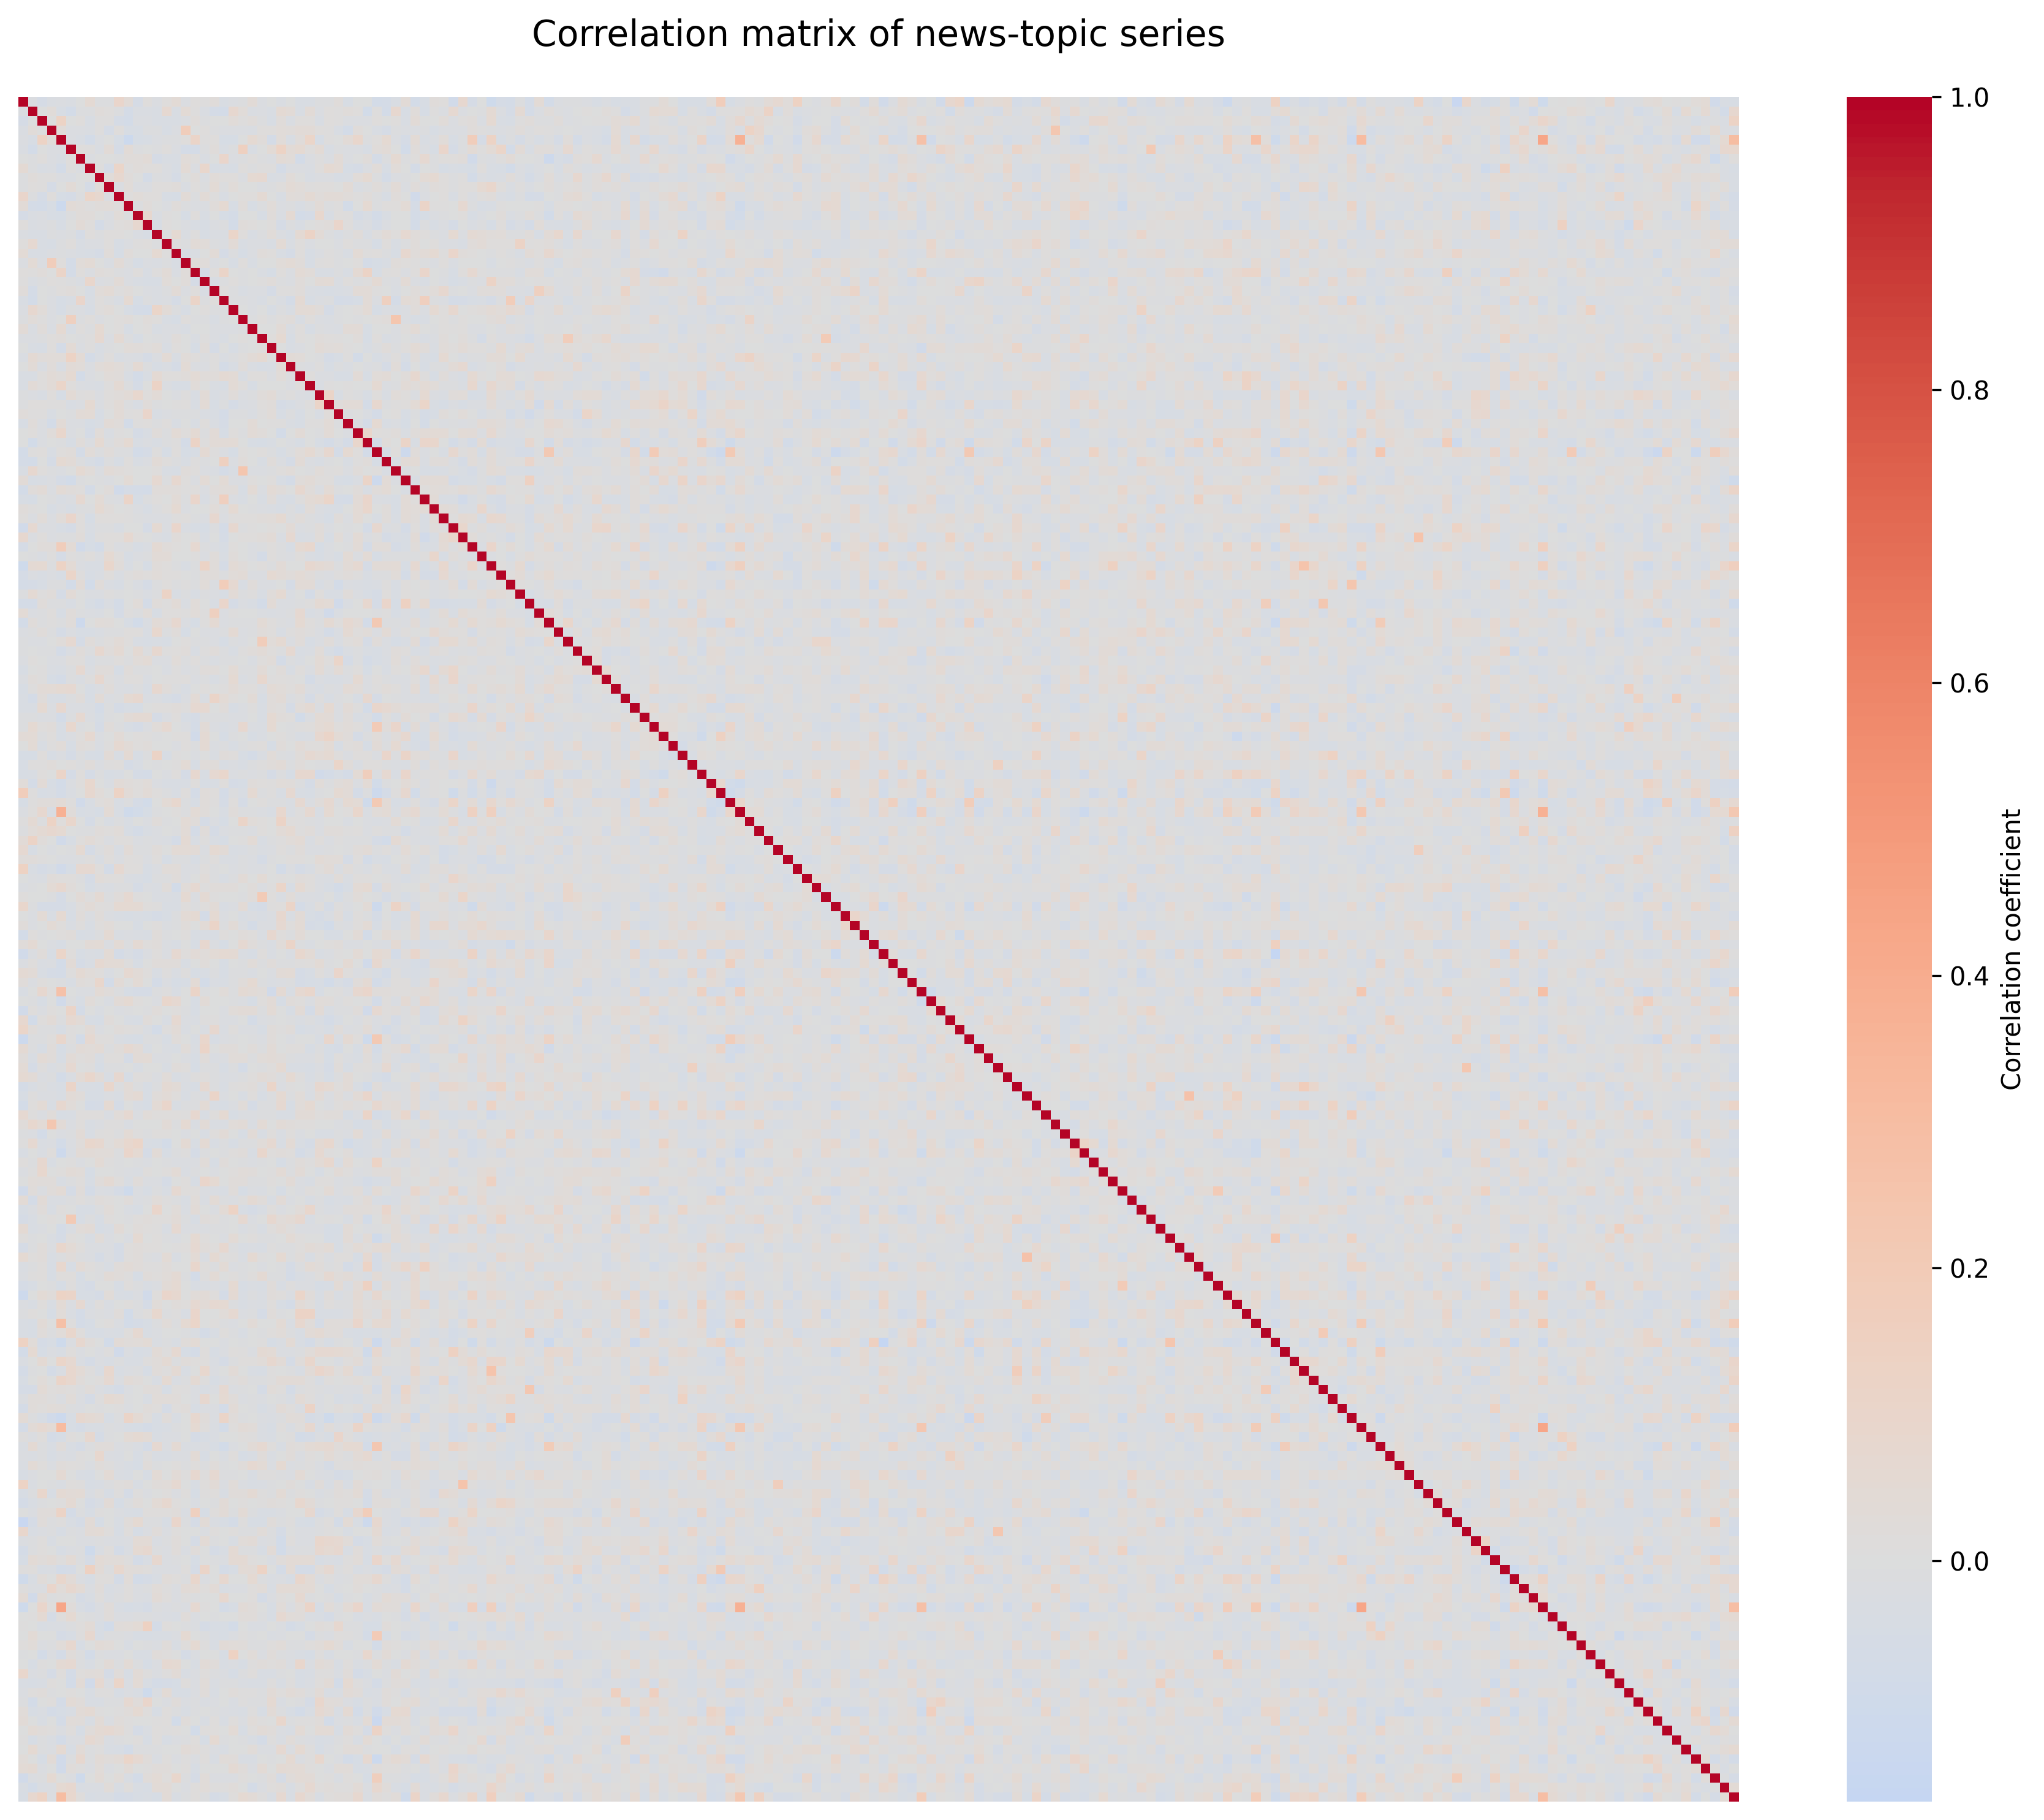
\includegraphics[width=\linewidth]{heatmap.png}
  \caption{Heatmap of correlation between news-topics.}
  \label{fig:corr_heatmap}
\end{figure}



\section{Oracle Test: Estimation on Model-Generated Data}\label{app:oracle}

As anticipated, there is no groundtruth for the hyperparamter lambda that governs how much investors use as penalty paramter.
To come up with a procedure to select lambda and to evaluate the performance of our two-stage estimation procedure, we conduct an oracle test using data generated from the ALM with known parameters.

We do this in two distinct flavours: first by assuming knowledge of the Stage-1 penalty $\lambda$, and then by tuning $\lambda$ via the same procedure we document below and that we use also in the empirical application.

We use the actual predictor matrix of empirical predictor innovations ($K=190$: 180 news-topic series and 10 macro-financial series) and simulate returns recursively from the ALM with
$\kappa_{\text{true}}=0.3$, $\lambda_{\text{true}}=6.625\times 10^{-5}$,
fixed window size $s=252$, and innovation volatility $\sigma=0.001$, over the full sample length of  $T=1{,}878$ daily periods accordingly to:
\[
r_{t+1}
= \log\!\bigl(1-\kappa e^{x_t^\top\hat\beta_t}\bigr)
- \log\!\bigl(1-\kappa e^{x_{t+1}^\top\hat\beta_{t+1}}\bigr)
+ \varepsilon_{t+1},
\qquad
\varepsilon_{t+1}\sim \mathcal{N}(0,\sigma^2).
\]



For the infeasible benchmark, Stage 1 is run with known true $\lambda$ and Stage 2 still
estimates $\kappa$ from simulated data.
As shown in the Infeasible column of Table~\ref{tab:oracle_optuna}, the infeasible oracle recovers $\kappa$ with a small error, and achieves a positive but modest Stage-2 fit both in-sample and out-of-sample.
The low $R^2$ values are expected and show that even when the representative investor's forecasting rule and penalty are correctly specified, returns remain close to an environment where predictability is weak and most variation is driven by the innovation term $\varepsilon_{t+1}$.

These results motivate a procedure to retrieve $\lambda$ from data alone. We search over a grid of values $\lambda \in [10^{-5},\,10^{-3}]$, 
to maximize the composite objective
\begin{equation}\label{eq:oracle_optuna_obj}
\text{Score}(\lambda)
= \frac{1}{3}\,\sigma\!\left(\hat\kappa_{t\text{-stat}} - 1.96\right)
+ \frac{1}{3}\,\exp\!\left(-\!\left(\frac{R^2_{\text{IS},1} - \bar R^2}{\delta}\right)^{\!2}\right)
+ \frac{1}{3}\,\sigma\!\left(\frac{R^2_{\text{IS},2}}{\eta}\right),
\end{equation}

where $\sigma(\cdot)$ is the logistic function, $R^2_{\text{IS},1}$ and $R^2_{\text{IS},2}$ are the Stage-1 and Stage-2 in-sample $R^2$, respectively. The three terms reward, in equal weight, $\kappa$ significance, a Stage-1 fit that is positive but not too large (bell centred at $\bar R^2 = 0.15$ with width $\delta = 0.08$), and positive Stage-2 in-sample fit (scale $\eta = 0.01$). We use in-sample $R^2$ for Stage 2 because the DGP is known, so overfitting is not a concern.
The maximization is done by using Tree-structured Parzen Estimation (TPE)\footnote{ TPE is a sequential model-based algorithm that at each iteration, partitiones past evaluations into a high-scoring set and a low-scoring set, fitting a separate density model to each. New candidates are proposed by sampling from the high-scoring density while down-weighting regions favoured by the low-scoring one, so the search progressively concentrates on values of $\lambda$ that yield higher composite scores. We use the implementation provided by the Optuna library for Python \citep{optuna_2019}. The number of trials is set to 150, which is sufficient for TPE to converge in a scalar search over $\lambda$: empirically, the objective stabilises well before 100 evaluations, and results are robust to varying the budget between 100 and 200 trials.} .

We report the comparison against the infeasible benchmark in Table~\ref{tab:oracle_optuna}.
The procedure selects $\hat\lambda = 7.56\times10^{-5}$, which is $1.14\times$ the true DGP value.
Despite this over-penalisation, $\kappa$ identification remains strong: $\hat\kappa = 0.372$ (absolute error $0.072$) with a $t$-statistic of $10.3$, compared to $\hat\kappa = 0.329$ (error $0.029$, $t = 9.6$) for the infeasible benchmark. 
The Stage-2 fit statistics are virtually identical across the two procedures ($R^2_{\text{IS},2} = 0.025$ in both cases; $R^2_{\text{OOS},2} = 0.029$ vs.\ $0.027$), 
We interpret these results as validating the composite tuning objective as a feasible procedure for $\lambda$ selection, since it
recovers a penalty which delivers a $\kappa$ estimate close to the infeasible benchmark.

\begin{table}[H]
\centering
\caption{Oracle Lambda Tuning: Infeasible vs.\ Composite Objective}
\label{tab:oracle_optuna}
\begin{tabularx}{0.8\textwidth}{@{}>{\small}l>{\small\centering\arraybackslash}X>{\small\centering\arraybackslash}X@{}}
\toprule
Metric & Infeasible & Composite Obj. \\
\midrule
$\lambda$ selected                & $6.63\times10^{-5}$ (known) & $7.56\times10^{-5}$ \\
$\lambda / \lambda_{\text{true}}$ & 1.000                       & 1.141 \\
$\hat\kappa$                      & 0.329                       & 0.372 \\
$|\hat\kappa - \kappa_{\text{true}}|$ & 0.029                  & 0.072 \\
$t$-stat($\hat\kappa$)            & 9.563                       & 10.322 \\
Stage-1 IS $R^2$                  & 0.188                       & 0.149 \\
Stage-1 OOS $R^2$                 & 0.003                       & 0.011 \\
Stage-2 IS $R^2$                  & 0.025                       & 0.025 \\
Stage-2 OOS $R^2$                 & 0.027                       & 0.029 \\
\bottomrule
\end{tabularx}
\medskip
\begin{minipage}{\textwidth}
\footnotesize
\textit{Note:} $K=190$ predictors (180 topics + 10 macro), $s=252$, $n_{\text{lags}}=1$, $\kappa_{\text{true}}=0.30$,
$\lambda_{\text{true}}=6.63\times10^{-5}$, $\sigma=0.001$.
The objective in equation~\eqref{eq:oracle_optuna_obj} is maximised over 150 TPE trials.
Stage-2 in-sample $R^2$ is used inside the objective because the DGP is known.
All estimation uses the same rolling-window LASSO plus NLS pipeline as the infeasible benchmark.
\end{minipage}
\end{table}

\section{Robustness: Feature Selection Among Significant-$\hat{\kappa}$ Stocks}\label{app:robustness_sig_kappa}

One might be concerned that the feature selection patterns documented in Section~\ref{sec:empirical} are driven by the large mass of low-volatility stocks for which the LASSO never selects any predictor.
To address this, we repeat the analysis of Section~\ref{subsec:empirical_belief_anatomy} restricting to the 155 stocks with a statistically significant $\hat{\kappa}$ estimate at the 5\% level.

The feature ranking is essentially unchanged.
The correlation between per-feature mean selection rates in the full sample and in the significant-$\hat{\kappa}$ subsample is $0.89$, and 7 of the top 10 features are identical across the two groups.
The top three features---\textit{Announce plan}, \textit{Financial reports}, and \textit{Germany}---are the same in both samples.
The Gini coefficient rises modestly from $0.18$ to $0.20$, reflecting a slight increase in concentration, but the overall distribution remains dispersed.
The macro-financial series show no systematic premium or discount relative to news topics in the restricted sample.

\paragraph{Persistence.}
We repeat the persistence analysis of Section~\ref{subsec:empirical_belief_anatomy} on the same 155 significant-$\hat{\kappa}$ stocks.
The results are nearly identical to the full sample.
Pooled across 69{,}760 selection episodes, the median run length is 4 windows and the 95th percentile is 78 windows, with a maximum of 481.
The survival curve declines from 73\% after one window to 18\% after 20 windows.
The first-order autocorrelation of the binary selection indicator, averaged across 9{,}708 active stock--feature pairs, is 0.89, decaying to 0.72 at lag 5 and 0.46 at lag 20.
Figure~\ref{fig:persistence_sig_kappa} plots the run-length distribution and survival curve for this subsample.

\begin{figure}[h]
    \centering
    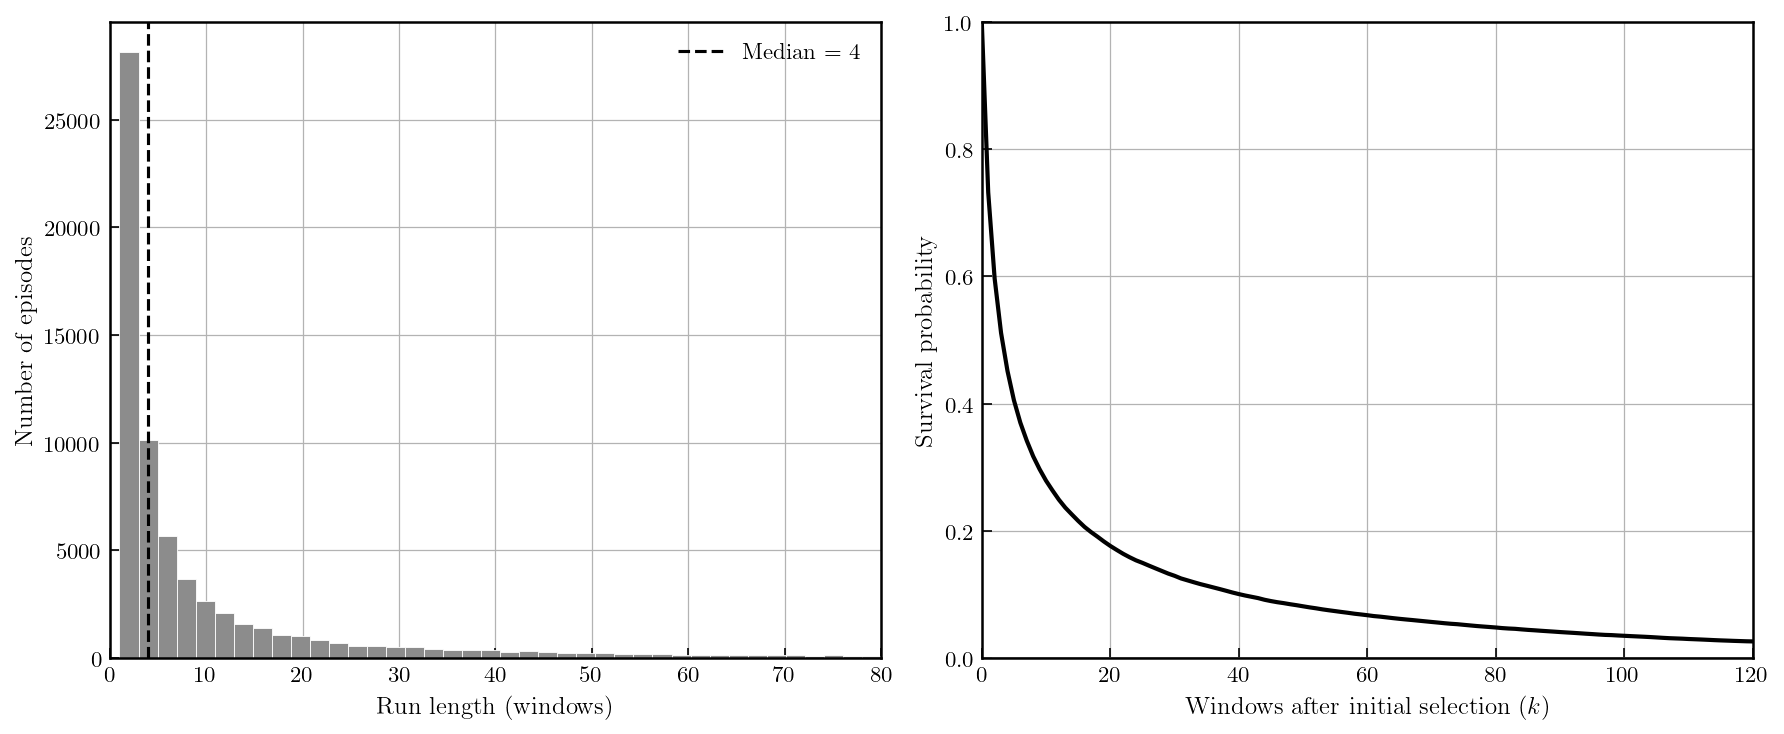
\includegraphics[width=\textwidth]{persistence_sig_kappa.png}
    \caption{Persistence of Topic Selection Episodes: Significant-$\hat{\kappa}$ Stocks}
    \label{fig:persistence_sig_kappa}
    \begin{minipage}{\textwidth}
    \footnotesize
    \textit{Note:} Same as Figure~\ref{fig:topic_selection_persistence} but restricted to the 155 stocks with a statistically significant $\hat{\kappa}$ estimate at the 5\% level.
    \textbf{Left panel}: run-length distribution truncated at 80 windows; dashed line marks the median ($=4$).
    \textbf{Right panel}: survival curve $P(\text{selected at }t+k \mid \text{selected at }t)$.
    \end{minipage}
\end{figure}

\subsection{Multiple-Testing Adjustments for Second-Stage Significance}\label{app:multiple_testing}

Because the second-stage ALM is estimated stock by stock, a natural concern is that some statistically significant $\hat{\kappa}_i$ estimates may arise from multiple testing rather than from systematic evidence in favour of the model.
To address this, we re-evaluate second-stage significance using the full set of 1{,}117 stocks for which a finite $\hat{\kappa}_i$ $t$-statistic is available in the baseline estimation output.
This is the broadest feasible comparison set for standard multiplicity corrections, because it includes every stock for which the nonlinear second-stage estimator returns a usable test statistic.

\begin{table}[H]
\centering
\caption{Multiple-Testing Corrections for Second-Stage $\hat{\kappa}_i$ Significance}
\label{tab:multiple_testing}
\begin{tabular}{lcc}
\toprule
Correction method & Rejections & Share of 1,117 tests \\
\midrule
Unadjusted 5\% level & 111 & 9.9\% \\
Benjamini--Hochberg FDR 10\% & 69 & 6.2\% \\
Benjamini--Hochberg FDR 5\% & 55 & 4.9\% \\
Holm--Bonferroni 5\% & 38 & 3.4\% \\
\bottomrule
\end{tabular}
\medskip
\begin{minipage}{0.92\textwidth}
\footnotesize
\textit{Note:} The table reports the number of second-stage ALM estimates for which the null $\kappa_i = 0$ is rejected after applying alternative multiple-testing adjustments to the 1{,}117 stocks with a finite $\hat{\kappa}_i$ $t$-statistic in the baseline estimation output. The Benjamini--Hochberg procedure controls the false discovery rate, while Holm--Bonferroni controls the family-wise error rate.
\end{minipage}
\end{table}

Table~\ref{tab:multiple_testing} shows that the number of significant second-stage estimates falls materially once multiplicity is taken into account, but a non-trivial subset of stocks remains significant even under conservative adjustments.

We also conduct a global excess-significance test.
Under the joint null that each stock-level test rejects with probability 5\%, the expected number of rejections among 1{,}117 tests is 55.9.
The observed count of 111 is almost exactly double that benchmark.
An exact binomial test for excess significance rejects strongly, with $p = 1.21 \times 10^{-11}$.
This result indicates that the aggregate number of significant second-stage estimates is too large to be explained by independent 5\% false positives alone.

The interpretation of these corrections is therefore nuanced.
They do not support reading every stock-level rejection as equally strong evidence for the model, and they imply that the raw count of unadjusted significant $\hat{\kappa}_i$ estimates overstates the amount of stock-by-stock evidence.
At the same time, the corrected results do not collapse to zero: depending on the criterion, between 38 and 69 stock-level rejections survive, and the global excess-significance test rejects decisively.
Taken together, these robustness checks suggest that the empirical support for the CMCE mechanism is concentrated in a smaller subset of stocks than the unadjusted 5\% count implies, but that the overall evidence is not well described as a pure multiple-testing artefact.

\end{document}
